%% This is the ctufit-thesis example file. It is used to produce theses
%% for submission to Czech Technical University, Faculty of Information Technology.
%%
%% Get the newest version from
%% https://gitlab.fit.cvut.cz/theses-templates/FITthesis-LaTeX
%%
%%
%% Copyright 2021, Eliska Sestakova and Ondrej Guth
%%
%% This work may be distributed and/or modified under the
%% conditions of the LaTeX Project Public Licenese, either version 1.3
%% of this license or (at your option) any later version.
%% The latest version of this license is in
%%  https://www.latex-project.org/lppl.txt
%% and version 1.3 or later is part of all distributions of LaTeX
%% version 2005/12/01 or later.
%%
%% This work has the LPPL maintenance status `maintained'.
%%
%% The current maintainer of this work is Ondrej Guth.
%% Contact ondrej.guth@fit.cvut.cz for bug reports.
%% Alternatively, submit bug reports into the tracker at
%% https://gitlab.fit.cvut.cz/theses-templates/FITthesis-LaTeX/issues
%%
%%

%%%%%%%%%%%%%%%%%%%%%%%%%%%%%%%%%%%%%%%%%
% CLASS OPTIONS
% language: czech/english/slovak
% thesis type: bachelor/master/dissertation
%%%%%%%%%%%%%%%%%%%%%%%%%%%%%%%%%%%%%%%%%
\documentclass[english,master,unicode]{ctufit-thesis}

%%%%%%%%%%%%%%%%%%%%%%%%%%%%%%%%%%
% FILL IN THIS INFORMATION
%%%%%%%%%%%%%%%%%%%%%%%%%%%%%%%%%%
\ctufittitle{Performance and robustness analysis of Bayesian filters} % replace with the title of your thesis
\ctufitauthorfull{Bc. Mykyta Boiko} % replace with your full name (first name(s) and then family name(s) / surname(s)) including academic degrees
\ctufitauthorsurnames{Boiko} % replace with your surname(s) / family name(s)
\ctufitauthorgivennames{Mykyta} % replace with your first name(s) / given name(s)
\ctufitsupervisor{Ing.\, Kamil Dedecius,\,Ph.D.} % replace with name of your supervisor/advisor (include academic degrees)
\ctufitdepartment{Department of Applied Mathematics} % replace with the department of your defence
\ctufityear{2022} % replace with the year of your defence
\ctufitdeclarationplace{Prague} % replace with the place where you sign the declaration
\ctufitdeclarationdate{\today} % replace with the date of signature of the declaration
\ctufitabstractCZE{
Jak je známo, stavové modely se široce používají k modelování různých pozorovatelných procesů v různých oblastech, od financí až po biologii. Na základě pozorované posloupnosti je hlavním zájmem odvodit posloupnost skrytých stavů, které je vyvolaly. Hlavním cílem této práce je studovat výkonnost a robustnost různých Bayesovských algoritmů používaných pro online filtraci stavů při dobře specifikovaných i chybně specifikovaných stavových modelech. Důvodem je skutečnost, že v praxi z různých důvodů často chybí znalost šumu procesu nebo měření. Tato práce se dotýká zejména poměrně populárního případu, kdy je model měření chybně specifikován. V rámci této práce je kladen důraz na seznámení s filtry z nejpopulárnější rodiny, Kalmanovy rodiny, a uvažuje se o nich z Bayesovského hlediska, přičemž nechybí ani částicový filtr, který je v souvislosti s aplikací na chybně specifikované modely považován za stabilnější. Pozornost bude věnována také a budou provedeny experimenty s tzv. přibližnými Bayesovskými filtry, které umožňují úplnou neznalost šumového rozdělení měření. Výsledkem práce by mělo být pokrytí teorie všeho výše uvedeného a výsledky experimentů, nevyjímaje stanovení plánů pro další rozvoj tématu.
}
\ctufitabstractENG{
As is well-known, state-space models are widely used to model different observable processes in various fields, from finance to biology. Based on the observed sequence, the main interest is to deduce the sequence of hidden states that gave rise to them. The primary goal of this thesis is to study the performance and robustness of various Bayesian algorithms used for online state filtering under both well-specified and misspecified state-space models. This is due to the fact that in practice, for various reasons, there is often a lack of knowledge of process noise or measurements. This thesis, in particular, touches on the rather popular case where the measurement model is misspecified. As part of this work, the emphasis is placed on an introduction to the filters from the most popular family, the Kalman family, and consider them from a Bayesian perspective, also not without the particle filter, which is regarded as more stable in the context of application to misspecified models. Attention will also be paid, and experiments will be conducted with so-called approximate Bayesian filters, which allow complete ignorance of the noise distribution of measurements. The result of the thesis should be the coverage of the theory of all of the above and the results of experiments, not excluding the definition of plans for the future development of this topic.
}
\ctufitkeywordsCZE{Stavový model, Kalmanova filtrace, částicový filtr, Approximate Bayesian Computation}
\ctufitkeywordsENG{State-space model, Kalman
filtering, particle filter, Approximate Bayesian Computation}
%%%%%%%%%%%%%%%%%%%%%%%%%%%%%%%%%%
% END FILL IN
%%%%%%%%%%%%%%%%%%%%%%%%%%%%%%%%%%

%%%%%%%%%%%%%%%%%%%%%%%%%%%%%%%%%%
% CUSTOMIZATION of this template
% Skip this part or alter it if you know what you are doing.
%%%%%%%%%%%%%%%%%%%%%%%%%%%%%%%%%%

\RequirePackage{iftex}[2020/03/06]
\iftutex % XeLaTeX and LuaLaTeX
    \RequirePackage{ellipsis}[2020/05/22] %ellipsis workaround for XeLaTeX
\else
    \RequirePackage[utf8]{inputenc}[2018/08/11] %this file encoding
    \RequirePackage{lmodern}[2009/10/30] % vector flavor of Computer Modern font
\fi

% hyperlinks
\RequirePackage[pdfpagelayout=TwoPageRight,colorlinks=false,allcolors=decoration,pdfborder={0 0 0.1}]{hyperref}[2020-05-15]

% uncomment the following to hide all hyperlinks
% \RequirePackage[pdfpagelayout=TwoPageRight,hidelinks]{hyperref}[2020-05-15]

\RequirePackage{pdfpages}[2020/01/28]

\setcounter{secnumdepth}{4} % numbering sections; 4: subsubsection



%%%%%%%%%%%%%%%%%%%%%%%%%%%%%%%%%%
% CUSTOMIZATION of this template END
%%%%%%%%%%%%%%%%%%%%%%%%%%%%%%%%%%


%%%%%%%%%%%%%%%%%%%%%%
% DEMO CONTENTS SETTINGS
% You may choose to modify this part.
%%%%%%%%%%%%%%%%%%%%%%
\usepackage{dirtree}
\usepackage{lipsum,tikz}
\usepackage{csquotes}
\usepackage{subfig} %subfigures
\usepackage{graphicx}

% http://mirrors.ibiblio.org/CTAN/macros/latex/contrib/biblatex-contrib/biblatex-iso690/biblatex-iso690.pdf
% variants: iso-numeric, iso-authoryear, iso-year
\usepackage[style=iso-authoryear]{biblatex}
\addbibresource{text/bib-database.bib}
\addbibresource{text/references.bib}
\usepackage{listings} % typesetting of sources
% \usepackage{minted} % typesetting of sources

% algorithm package
\usepackage{algorithm,algcompatible,amsmath}
\DeclareMathOperator*{\argmax}{\arg\!\max}% https://tex.stackexchange.com/q/83169/5764
\algnewcommand\INPUT{\item[\textbf{Input:}]}%
\algnewcommand\OUTPUT{\item[\textbf{Output:}]}%

%theorems, definitions, etc.
\theoremstyle{plain}
\newtheorem{theorem}{Theorem}
\newtheorem{lemma}[theorem]{Lemma}
\newtheorem{corollary}[theorem]{Důsledek}
\newtheorem{proposition}[theorem]{Návrh}
\newtheorem{definition}[theorem]{Definice}
\theoremstyle{definition}
\newtheorem{example}[theorem]{Příklad}
\theoremstyle{remark}
\newtheorem{note}[theorem]{Poznámka}
\newtheorem*{note*}{Poznámka}
\newtheorem{remark}[theorem]{Pozorování}
\newtheorem*{remark*}{Pozorování}
\numberwithin{theorem}{chapter}
%theorems, definitions, etc. END
%%%%%%%%%%%%%%%%%%%%%%
% DEMO CONTENTS SETTINGS END
%%%%%%%%%%%%%%%%%%%%%%

\begin{document} 
\frontmatter\frontmatterinit % do not remove these two commands

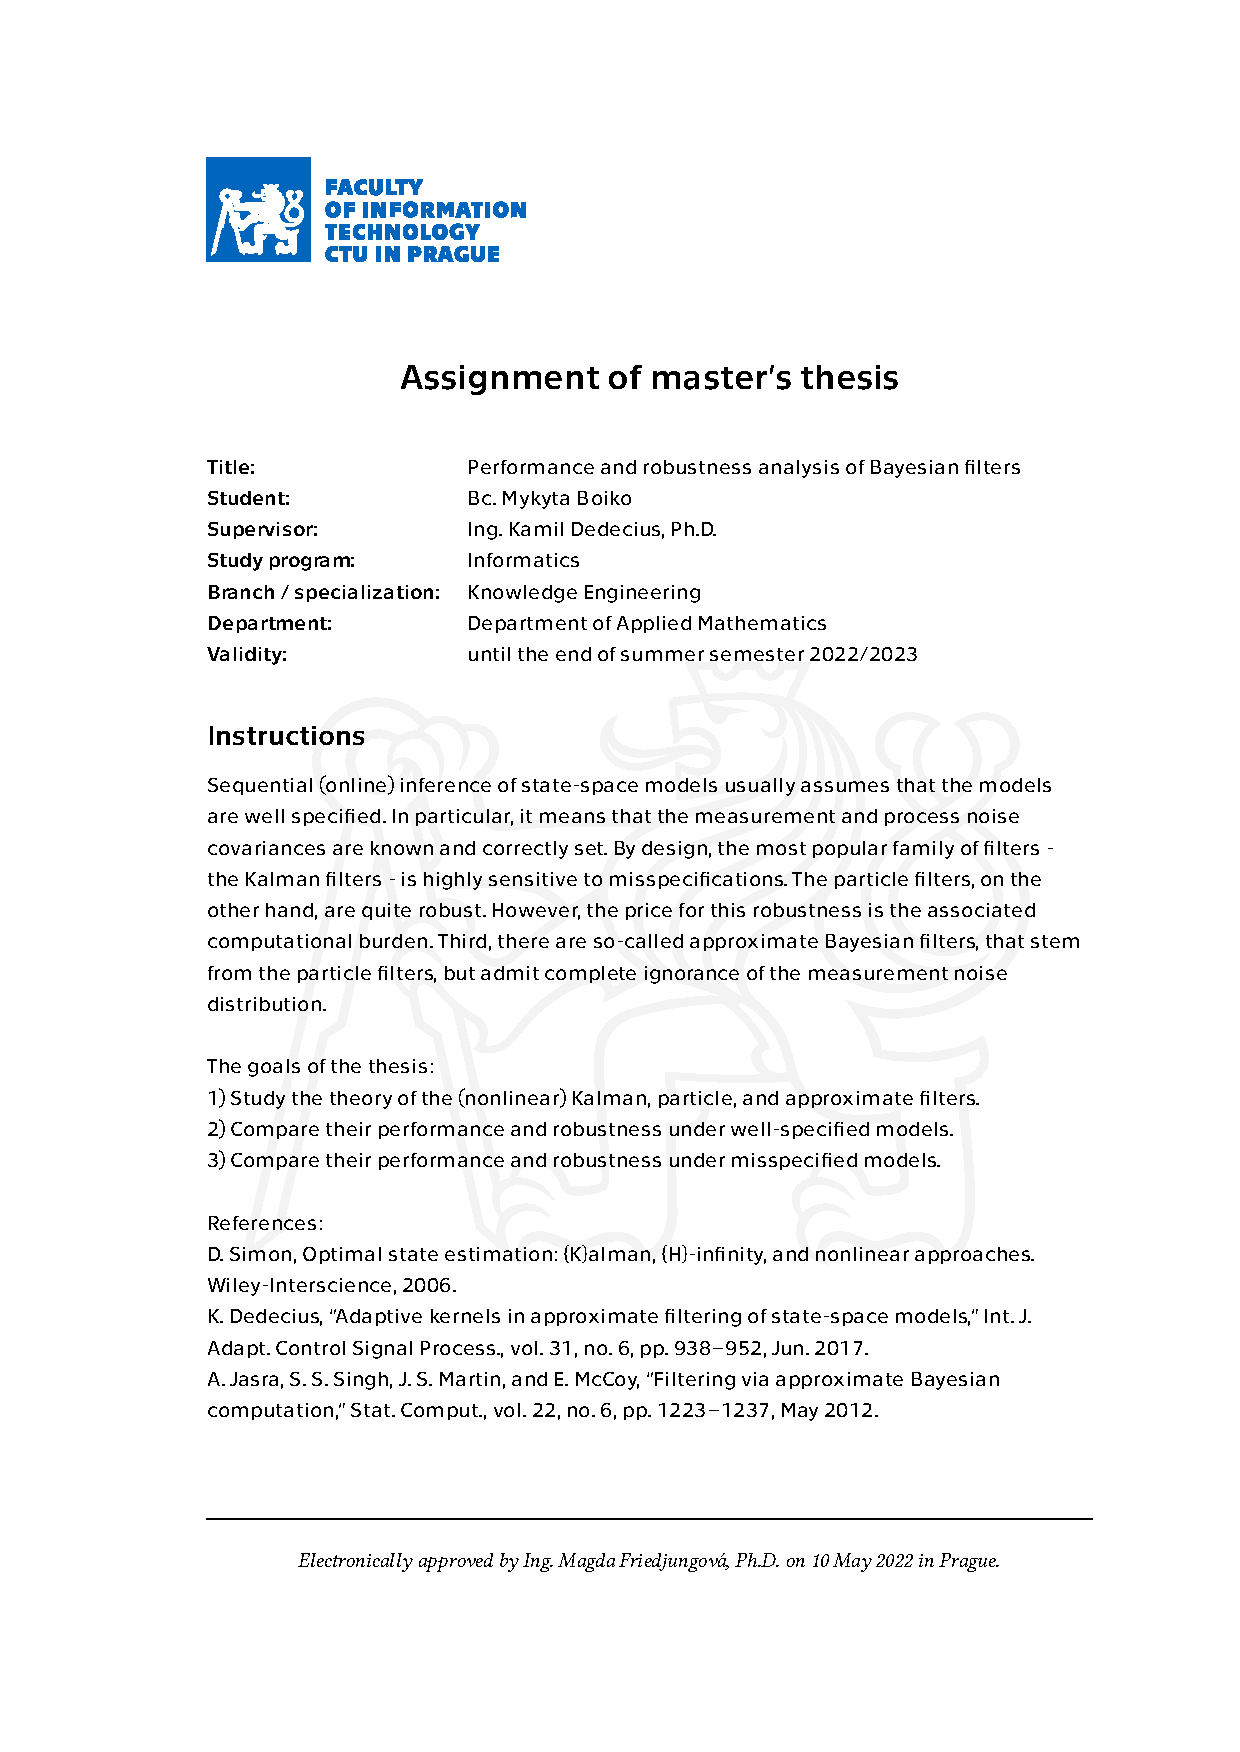
\includepdf{boikomyk-assignment.pdf} % replace that file with your thesis assignment provided by study office

\thispagestyle{empty}\cleardoublepage\maketitle % do not remove these three commands

\imprintpage % do not remove this command

\tableofcontents % do not remove this command
%%%%%%%%%%%%%%%%%%%%%%
% list of other contents: figures, tables, code listings, algorithms, etc.
% add/remove commands accordingly
%%%%%%%%%%%%%%%%%%%%%%
\listoffigures % list of figures
\begingroup
\let\clearpage\relax
\listoftables % list of tables
\lstlistoflistings % list of source code listings generated by the listings package
% \listoflistings % list of source code listings generated by the minted package
\endgroup
%%%%%%%%%%%%%%%%%%%%%%
% list of other contents END
%%%%%%%%%%%%%%%%%%%%%%

%%%%%%%%%%%%%%%%%%%
% ACKNOWLEDGMENT
% FILL IN / MODIFY
% This is a place to thank people for helping you. It is common to thank your supervisor.
%%%%%%%%%%%%%%%%%%%
\begin{acknowledgmentpage}
	I want to thank my supervisor Kamil Dedecius for his responsiveness, ability to interest the topic, and curatorial work. I would also like to express my gratitude to my parents.
\end{acknowledgmentpage} 
%%%%%%%%%%%%%%%%%%%
% ACKNOWLEDGMENT END
%%%%%%%%%%%%%%%%%%%


%%%%%%%%%%%%%%%%%%%
% DECLARATION
% FILL IN / MODIFY
%%%%%%%%%%%%%%%%%%%
% INSTRUCTIONS
% ENG: choose one of approved texts of the declaration. DO NOT CREATE YOUR OWN. Find the approved texts at https://courses.fit.cvut.cz/SFE/download/index.html#_documents (document Declaration for FT in English)
% CZE/SLO: Vyberte jedno z fakultou schvalenych prohlaseni. NEVKLADEJTE VLASTNI TEXT. Schvalena prohlaseni najdete zde: https://courses.fit.cvut.cz/SZZ/dokumenty/index.html#_dokumenty (prohlášení do ZP)
\begin{declarationpage}
I hereby declare that the presented thesis is my own work and that I have cited all sources of information in accordance with the Guideline for adhering to ethical principles when elaborating an academic final thesis.
I acknowledge that my thesis is subject to the rights and obligations stipulated by the Act No. 121/2000 Coll., the Copyright Act, as amended, in particular that the Czech Technical University in Prague has the right to conclude a license agreement on the utilization of this thesis as a school work under the provisions of Article 60 (1) of the Act.
\end{declarationpage}
%%%%%%%%%%%%%%%%%%%
% DECLARATION END
%%%%%%%%%%%%%%%%%%%

\printabstractpage % do not remove this command

%%%%%%%%%%%%%%%%%%%
% SUMMARY
% FILL IN / MODIFY
% OR REMOVE ENTIRELY (upon agreement with your supervisor)
% (appropriate to remove in most theses)
%%%%%%%%%%%%%%%%%%%
% \begin{summarypage}
% \section*{Summary section}

% \lipsum[1][1-8]

% \section*{Summary section}

% \lipsum[2][1-6]

% \section*{Summary section}

% \lipsum[3]

% \section*{Summary section}

% \lipsum[2]

% \section*{Summary section}

% \lipsum[1][1-8] Lorem lorem lorem.
% \end{summarypage}
%%%%%%%%%%%%%%%%%%%
% SUMMARY END
%%%%%%%%%%%%%%%%%%%

%%%%%%%%%%%%%%%%%%%
% ABBREVIATIONS
% FILL IN / MODIFY
% OR REMOVE ENTIRELY
% List the abbreviations in lexicography order.
%%%%%%%%%%%%%%%%%%%
% \chapter{Acronyms}
	
% \begin{tabular}{rl}
% DFA & Deterministic Finite Automaton\\
% FA & Finite Automaton\\
% LPS & Labelled Prüfer Sequence\\
% NFA & Nondeterministic Finite Automaton\\
% NPS & Numbered Prüfer Sequence\\
% XML & Extensible Markup Language\\
% XPath & XML Path Language\\
% XSLT & eXtensible Stylesheet Language Transformations\\
% W3C & World Wide Web Consortium
% \end{tabular}
%%%%%%%%%%%%%%%%%%%
% ABBREVIATIONS END
%%%%%%%%%%%%%%%%%%%

\mainmatter\mainmatterinit % do not remove these two commands

%%%%%%%%%%%%%%%%%%%
% THE THESIS
% MODIFY ANYTHING BELOW THIS LINE
%%%%%%%%%%%%%%%%%%%


%---------------------------------------------------------------
% Introduction
% Do not forget to include Introduction
%---------------------------------------------------------------
% \chapter{Introduction}
% uncomment the following line to create an unnumbered chapter
\chapter*{Introduction}\addcontentsline{toc}{chapter}{Introduction}\markboth{Introduction}{Introduction}
%---------------------------------------------------------------
\setcounter{page}{1}

It is hard to deny that the world is, in one way or another, entirely made up of dynamic systems. A dynamic system is always characterized by a state that changes or evolves over time. This thesis examines the state-space modeling approach of such dynamic systems, or more precisely,  of time series. State space representation is quite popular and widely used in various fields, such as economics, ecological modeling, engineering, etc.

This thesis considers the sequential inference of state-space models using the universal Bayesian framework, which consists of finding the posterior distribution of the states based on the initial belief, or more correctly put, the prior density and observed sequence, which acts as a correcting factor. Of course, this includes a detailed review of the theoretical basis on which Bayesian methods are built, and not without filters from the most popular family of filters, Kalman filters, which are direct analytical implementations of Bayesian principles. On the one hand, for more convenience and simplicity within the limits of linear systems, the standard Kalman filter, which is an efficient linear estimator, and under some conditions, even the best linear filter, will be analyzed in detail. On the other hand, taking into account that in the real world, linear systems almost do not exist because real systems always have some non-linearities, to overcome the accompanying non-linear problems also on the agenda will be its extended version.

Unfortunately, the above methodology and filters are based on the fact that both models, the process model and the model generating the measurements, are always well known, that is, represented in the form of well-defined probability density functions. In practice, however, it can often be found a situation where the model is poorly specified, or in general, the correct model is not available. This can be caused by various reasons, both trivial lack of knowledge of the domain and difficulties associated with numerical calculations. This thesis deals with the rather common situation when the measurement model is misspecified, which may be the case if the likelihood function of the state-space model is analytically intractable, for example.

At this point, attention will be redirected to a class of sequential Monte Carlo filters called particle filters, which also, like Kalman filters, require full model specification, but, unlike them, based on numerous studies in particle filtering associated with misspecification issues, they are known to be quite robust even in such cases. Also, attention will not be ignored to the question of the price they pay for this notorious stability, which will be directly related to the analysis of the principle of their work. Under special consideration will also be their approximate extensions, the so-called approximate Bayesian filters, which allow one to completely ignore the noise distribution of measurements.

Among the main objectives of the work are the following points:
\begin{itemize}
    \item An in-depth study of the theory of all the above filters and methodologies.
    \item Conduct experiments on both well-specified models and misspecified models to compare performance and robustness of different filters.
\end{itemize}

As for the organization of the thesis, it is as follows. The Chapter \ref{chap:ssm_and_estimation} will be an introduction to the world of state-space modeling, which will begin with a historical introduction about the reasons and motivations for its use. In addition, the assumed form of a state-space model will be properly defined, followed by a transition to Bayesian filtering background and a discussion of the methodology itself, followed by an explanation of how these can be applied to state-space models. All this will be followed by a presentation of the concept of the Kalman filter from a Bayesian perspective, as well as its extended version for non-linear cases, with a gradual transition to the class of filters from the family of sequential Monte Carlo methods. Toward the end, the topic of the particle filter and its approximate extensions are touched upon, which directly includes the analysis of the ABC methodology.

After that, the practical part follows, namely that all the filters described above will take part in the experiments. In Chapter \ref{chap:well_specified}, this goal will be directed to the study of the efficiency of filters under the conditions of well-specified models. This chapter deals with several models, there are both linear and non-linear models. The Chapter \ref{chap:misspecified} will also focus on numerical studies, but this time the experiments will be carried out on misspecified models.

And finally, Chapter \ref{chap:conclusion} concludes the whole thesis and also sets possible directions for future work.

\section*{Personal motivation}
It would also be nice to add a few words about personal motivation. One of the main reasons was that the author of this work had a fairly general idea, or rather a lot of gaps in knowledge about the Kalman filter, etc. So it was quite an exciting challenge and an opportunity to go deeper, to get acquainted with the concept of Bayesianism, and maybe even in the future, to somehow connect work plans with it. At a minimum, the author does not regret the chosen topic and is very pleased with the knowledge gained in this thesis.
%---------------------------------------------------------------
% State-space models and their estimation
%---------------------------------------------------------------
\chapter{State-space models and their estimation}
\label{chap:ssm_and_estimation}
%---------------------------------------------------------------

\begin{chapterabstract}
"We may regard the present state of the universe as the effect of its past and the cause of its future" – Marquis de Laplace
\end{chapterabstract}

This chapter begins with a historical summary and basic understanding of key terms, both new and simply expanding on those already mentioned in the introduction section.
They must cover all aspects of the work that follows, in particular, to facilitate the further construction of theory in the following sections. In addition, the reader should become familiar with them for a better understanding, and unproblematic tracing of the logical chains encountered in some parts of the work. Later, the chapter expands and deepens into technical details that structurally complement the overall work.

\section{Historical development}

We are surrounded by physical dynamic systems all around us. The main difference from static systems is that the relationship between the inputs and outputs changes with time and depends on past inputs and initial conditions. Also, the relationship is represented by a differential equation, not an algebraic equation. The range of dynamic systems problems is extensive. We meet with them in statistics, engineering, economics, ecology, and many others.
It should be said that the basic concept in a dynamical system is state \(x\), which holds core information about the system and, in most cases, changes over time. The state \(x(t_1)\) at any future time, may be determined exactly given knowledge of the initial state, \(x(t_0)\) and the time history of the inputs,\(u(t)\) between \(t_0\), and \(t_1\). In general, the state information is not available directly. Such a state, we name hidden. Instead, we have some observable measurements \(y\), taken at specific times, that directly relate to the state.
Various statistical methods and approaches can be used to analyze such systems. The purpose is to obtain specific characteristics and descriptions through data interpretation. Subsequently, a suitable model characterizing system state and time evolution can be built based on received data. Such a model can be used both to simulate data and to predict future states of the system.

The state space approach was firstly introduced by \textcite{kalman_new_1960} and \textcite{zadeh_linear_1963} in the control engineering area. That was the beginning of the modern control theory, which is based on the state representation of systems in the time domain. Such representation is what makes it different from the classical control theory. It is worth noting that classical control mainly applies to LTI\footnote{Linear time-invariant} SISO\footnote{Single Input Single Output} CT\footnote{Continuous-time} systems using the Laplace transform to model such systems as transfer functions. In contrast, the modern one extends SISO to MIMO\footnote{Multi Input Multш Output}, both CT and DT\footnote{Discrete-time}.

The state space modeling approach is a matrix method that rearranges large-order differential equations as a series of first-order differential equations. The state-space methodology is capable of modeling systems with a large number of degrees of freedom, as well as systems with nonlinearities. Moreover, it is worth saying that the state space model can cover a widespread class of dynamic models.

In essence, the first SSMs, often called NDLMs\footnote{Normal dynamic linear model}, were a case where the state and the observation time series were modeled with linear equations and normal distributions. Two fundamental papers on NDLMs, the previously mentioned \textcite{kalman_new_1960} and \textcite{zadeh_linear_1963}, provided an algorithmic method, well-known to us Kalman filter, which makes for inferencing the hidden states gave imperfect observations and known parameters.
These works played a crucial role in aerospace technology in the 1960s. Related developments helped to adjust the trajectory of the Apollo mission to the Moon to account for inaccurate observations of the spacecraft's position over time (\textcite{grewal_applications_2010}). It can be said, that corresponding model arose in the space tracking conditions, where the state equation defines the motion equations for the state of a spacecraft with location \(x_t\) and the data \(y_t\) carry in them such information as velocity and azimuth that can be observed from a tracking device.

It should be clear that NDLMs are a limited class of SSMs and their applicability to physical dynamic systems, which have nonlinear and non-Gaussian structures, is limited. In addition, unlike the planned mission to the Moon, we rarely have a priori knowledge of the required parameters of physical systems. Incidentally, developments in the time series literature used the Kalman filter to estimate a likelihood function for unknown parameters, which in turn allowed maximum likelihood parameter estimates to be computed in addition to state estimates (\textcite{harvey_forecasting_1990}).

The situation changed in 1990s, with the popularization of Markov chain Monte Carlo (MCMC) methods (\textcite{gilks_markov_1995}), also including the freely available BUGS\footnote{Bayesian inference Using Gibbs Sampling} software(\textcite{lunn_bugs_2009}) and the advent of high-speed desktops. The variety of possible SSMs expanded considerably, including non-Gaussian and nonlinear formulations.

Summarizing what has been written above, it can be said that state-space models, or as they are often called hidden Markov models (HMM),  are characterized by two primary conditions. The first one is that there is a hidden or latent process \(x_t\) called the state process. The state process is assumed to be a Markov process. This simply means that the future \(\{x_s ; s > t\}\), and past \(\{x_s ; s < t\}\), are independent conditional on the present, \(x_t\) . The second prerequisite is that the observations \(y_t\) are independent given the states \(x_t\). It means that states generate dependence on the observations. The process can be specified by one or more latent variables, called state variables, that contain all knowledge to obtain information about the current state.
So, in other words, a need to control or predict the future of a system should be sufficient knowledge of the current system state, which can, for example, be obtained with a Kalman filter and its future input. If the state does not contain enough information, the latent number of state variables must be expanded until it does. In the sense indicated above, the state of the state space model provides a complete latent description of the system at any point in time (\textcite{willems_introduction_1997}). This could explain the considerable popularity of the state-space model and its usefulness in forecasting and control problems.


\section{State-space models}

As mentioned earlier, we have a Markov process at the core of the state-space model. Generally, the model is described by two parallel linked processes that evolve over time and are represented as conditional distributions. It assumes latent states \(\{x_t\}^\infty_{t=0} \subseteq \mathbb{R}^{n_x} \) following a Markov chain, where \(t = 0,...,T\) is the index most commonly representing time in time-series data, but other interpretations are also allowed. The state \(x_t\) represents the physical state of an object under study. It can be expressed as the position or coordinates of the flying airplane, direction and acceleration of the vehicle, animal movement trajectories, and others. Also, it is worth understanding that the state may be an abstract representation without any apparent physical interpretation.  

It is worth emphasizing that in this context the Markov property is fulfilled, that is: current state of the process \(x_t\) is fully enough to predict the future state of the process \(x_{t+1}\) and the prediction should be as good as making prediction by knowing their history \(...,x_{t-1}\), i.e.,

\begin{equation}
p(x_t \mid ...,x_{t-2},x_{t-1}) = p(x_t \mid x_{t-1}) \label{eq:markov_assumption}
\end{equation}

Such a condition, when each state is conditionally independent of its non-descendants, given its parents, is called Markov assumption and that is the key for efficiency when learning state-space models.

Also, the state-space model assumes a sequence of observed variables \(\{y_t\}^\infty_{t=1} \subseteq \mathbb{R}^{n_y} \). Through out this thesis, for a fixed time \(T \geq 1 \), we are going to use the following short-hands: \(x_{0:T} = \{x_t\}^T_{t=0}\) and \(y_{1:T} = \{y_t\}^T_{t=1}\). 

Now, having the right connotation, we can define the SSM  in three probability distributions as follow:

\begin{subequations}
\begin{align}
 x_t \mid x_{t-1}  &\sim f(x_t \mid x_{t-1}) \label{eq:ssm_in_probabilities_subeq_evolution} \\
 y_t \mid x_t  &\sim g(y_t \mid x_t) \label{eq:ssm_in_probabilities_subeq_measurement} \\
 x_0 &\sim p(x_0) \label{eq:ssm_in_probabilities_subeq_prior_initial_state}
\end{align}
\label{eq:ssm_in_probabilities}
\end{subequations}

\noindent where \(f(\cdot \mid \cdot)\) and \(g(\cdot \mid \cdot )\) are scalar or multivariate (stochastic) state(alternatively system, evaluation, transition) and observation (alternatively measurement, output) functions, respectively.
The state function describes an evolution in the states between time \(t\) and previous time \(t-1\) and the observation function describes the a relation between the state \(x_t\) and the related observation \(y_t\). These functions may be linear or nonlinear. To put it in a Bayesian context, they are conditional probability densities, expressing the stochastic nature of the considered processes. It is important to note, that the Markov property does not necessarily satisfied for the observations. For completeness, the model definition should also include a prior distribution of the initial state \(x_0\), which is given by \(p(x_0)\). Furthermore, to describe both: the evolution of the states and the available, a probabilistic approach is used.

\begin{figure}[!ht]
\centering
\caption{Graphical representation of the state-space model}
\subfloat{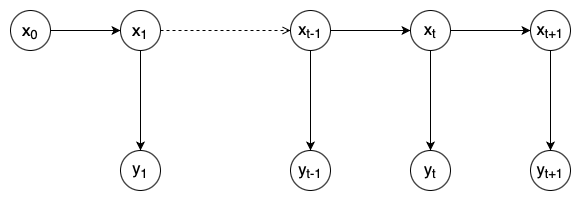
\includegraphics[width=0.8\columnwidth]{figures/SSM_graphical_representation}}
\label{fig:SSM_graphical_representation}
\end{figure}

An alternative name for the model described by the distributions above (\ref{eq:ssm_in_probabilities}) is hidden Markov model, where the word \emph{hidden} refers to the unobserved states \(x_t\) that, as already mentioned earlier, obey the Markov assumption (\ref{eq:markov_assumption}). Also, in some literature, this term is used concerning models where \(x_t\) exists in discrete space instead of in \(\mathbb{R}^{n_x} \). Figure \ref{fig:SSM_graphical_representation} shows the dependence relationship between the hidden unobserved state and observed data.


Another variation of (\ref{eq:ssm_in_probabilities}) is the time-varying state-space model, where  \(f(\cdot \mid \cdot)\) and \(g(\cdot \mid \cdot )\) and possibly also \(n_x\) depend explicitly on \(t\). Also, in the automatic control literature, state-space models are often used with the addition of an exogenous and known input signal \(u_t \in \mathbb{R}^{v}\).

When asking why to use state-space modeling and why the representation of systems in state-space is helpful, there are a couple of main points to be made:
\begin{itemize}
    \item Putting the systems into state space, essentially matrix forms, is a big advantage because computers were good with numbers but bad with symbolic computation
    \item The states have a physical meaning, that is speed or coordinates of airplane, that is of interest
    \item In terms of constructing predictions. The states \(x_t\) represent a compact summary of the whole relevant history. Provided that the Markov assumption is satisfied for states \(x_t\), it is enough to consider \(x_t\) for predicting the future observations \(y_{t+1}\) than to store and process all the historical data \(y_1, . . . , y_t\)
\end{itemize}

Rather popular subclass of model (\ref{eq:ssm_in_probabilities}) is the following:

\begin{subequations}
\begin{align}
    x_t &= G(x_{t-1}) + \omega_t \\
    y_t &= F(x_t) + \nu_t
\end{align}
\label{eq:ssm_subclass}
\end{subequations}

\noindent where \(F(\cdot)\) and \(G(\cdot)\) are the state and the observations functions respectively. Each equation contain noise component, \(\omega_t\) is defined as the state noise process and \(\nu_t\) as the observation noise process.

\subsection{Linear state-space models}

We will examine the linear models on the probably most famous and well-studied Gaussian SSM with additive noise, also called the dynamic linear model (DLM).

\begin{subequations}
\begin{alignat}{2}
    x_t = A_t x_{t-1} + B_t u_t + \omega_t \qquad \omega_t \sim \mathcal{N}(0, Q_t), \\
    y_t = C_t x_t + D_t u_t +  \nu_t   \qquad \nu_t \sim \mathcal{N}(0, R_t)
\end{alignat}
\label{eq:ssm_gaussian}
\end{subequations}

The main primitives of the model are:
\begin{itemize}
    \item \(x_t\) is a \(n \times 1\) vector consisting of unobserved variables (states) at time \(t\),
    \item \(y_t\) is a scalar univariate sequence of observed variables at time \(t\),
    \item \(A_t\) is a \(n \times n\) \textbf{transition or update matrix} which describes the evolution in the states at time t,
    \item \(C_t\) is a \(n \times 1\) \textbf{output or extraction matrix}  at time t,
    \item \(\omega_t\) is the term of evolution error. It is noise describing stochastic changes in the unobserved state, i.i.d with respect to time, with uncertainty covariance variance matrix \(Q_t\),
    \item \(\nu_t\) is a term of observational noise. It represents a measurement error and is also i.i.d with respect to time, with uncertainty covariance variance matrix \(R_t\).
\end{itemize}

Typically the \(D_t\) matrix is equal to zeros because the input signal do not typically affect the output directly. The \(C_t\) matrix is often one of the states, or sometimes it is just the identity matrix. To fit the standard notation in the systems identification literature, we shifted from the probabilistic notation and included an exogenous input signal \(u_t\) with related matrices \(B_t\) and \(D_t\) of appropriate sizes.

The main conditions that must be met to obtain a Gaussian SSM from a general SMM are that linearity is preserved for \(f(\cdot \mid \cdot)\) and \(g(\cdot \mid \cdot )\) functions, and both noise processes \(\omega_t\) and \(\nu_t\) are Gaussian. Simply put, the relationship between states, and between observation and states, are linear.

\subsubsection{Examples}

In this subsection we give several examples of state-space model development for linear physical systems and break them down.

\paragraph{Example 1 - Angular acceleration of a motor}
{\em
"As an example of a linear system, suppose that we are controlling the angular acceleration of a motor (for example, with some applied voltage across the motor windings). The derivative of the position is the velocity. A simplified motor model can then be written as:

\begin{subequations}
\begin{align*}
    \theta &= \omega \\
    \omega &= u + \omega_1
\end{align*}
\end{subequations}

The scalar \(w_1\) is the acceleration noise and could consist of such factors as uncertainty in the applied acceleration, motor shaft eccentricity, and load disturbances. If our measurement consists of the angular position of the motor then a state space description of this system can be written as:

\begin{subequations}
\begin{align*}
    x =
    \begin{bmatrix}
        \theta \\
        \omega
    \end{bmatrix}
    &=
    \begin{bmatrix}
        0 & 1 \\
        0 & 0
    \end{bmatrix}
    \begin{bmatrix}
        \theta \\
        \omega
    \end{bmatrix}
    +
    \begin{bmatrix}
        0 \\
        1
    \end{bmatrix}
    u + 
    \begin{bmatrix}
        0 \\
        \omega_1
    \end{bmatrix}
    \notag \\
    y = 
    \begin{bmatrix}
        \theta
    \end{bmatrix}
    &=
    \begin{bmatrix}
        1 & 0 \\
    \end{bmatrix}
    x + v
\end{align*}
\end{subequations}

The scalar \(v\) consists of measurement noise. The state vector \(x\) is a \(2 \time 1\) vector containing the scalars \(\theta\) and \(\omega\)."
} \cite[page~20]{simon_optimal_2006}

\paragraph{Example 2 - Mass-spring damper}
{\em

\begin{figure}[!ht]
\centering
\caption{Evolution of a damped mass-spring system}
\subfloat{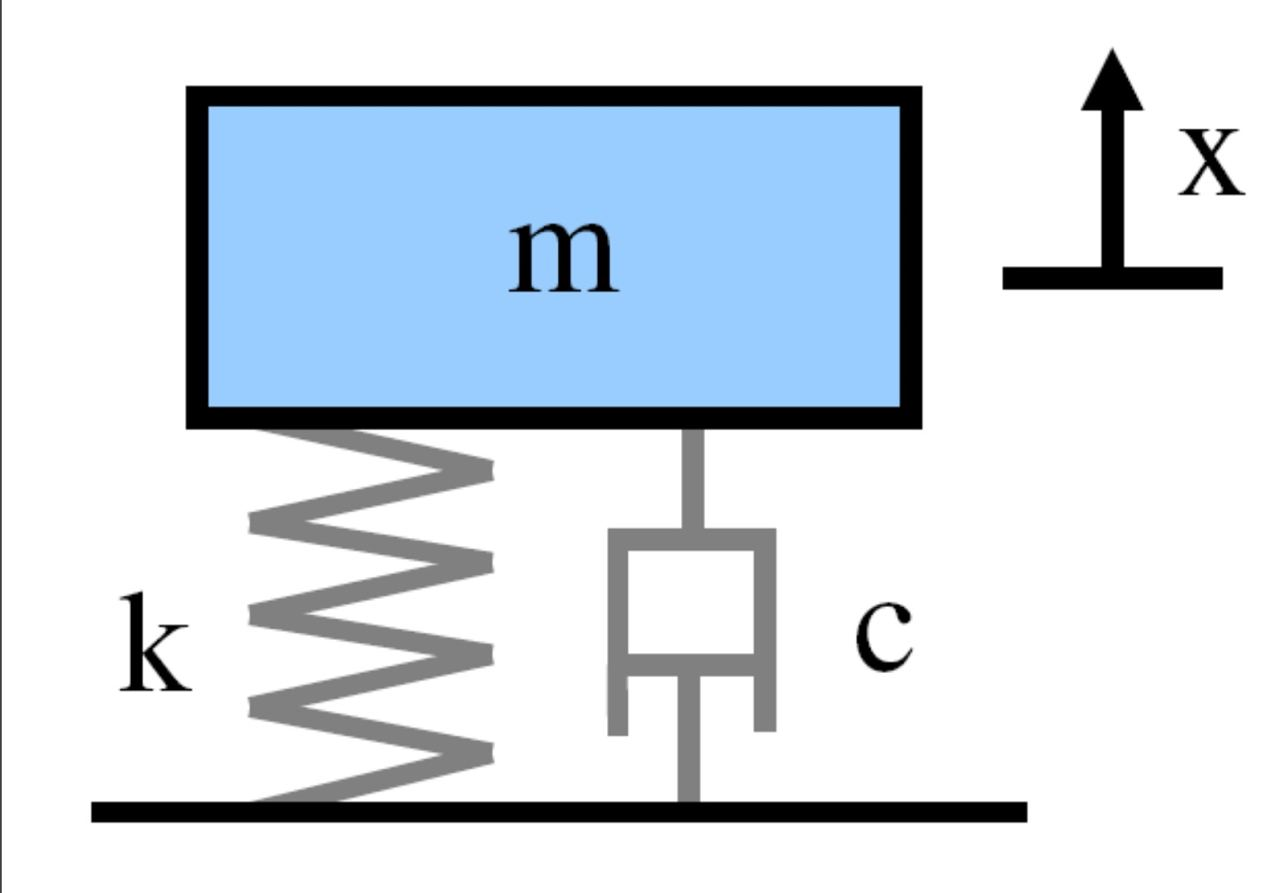
\includegraphics[
width=0.5\columnwidth,
height=4cm
]{figures/mass_spring_damper.jpg}}
\label{fig:SSM_graphical_representation}
\end{figure}

"Consider for example the second-order differential equation:
\begin{equation*}
my''_t + cy'_t + ky_t = u_t
\end{equation*}

which describes the evolution of a damped mass-spring system, with u the external force acting on the mass, and y the vertical position. (Here \(y'\) and \(y''\) are the first and second derivatives of y, respectively.)

The above involves second-order derivatives of a scalar function \(y(\cdot)\). We can express it in an equivalent form involving only first-order derivatives, by defining the state vector to be

\begin{equation*}
x_t =
    \begin{bmatrix}
        y_t \\
        y'_t
    \end{bmatrix}
\end{equation*}

The price we pay is that now we deal with a \textit{vector} equation instead of a scalar equation:

\begin{equation*}
x_t =
    \begin{bmatrix}
        0 & 1 \\
        -\frac{c}{m} & -\frac{k}{m}
    \end{bmatrix}
    x_t +
        \begin{bmatrix}
        0 \\
        1
    \end{bmatrix}
    u_t
\end{equation*}

The position \(y_t\) is a linear function of the state:

\begin{equation*}
y_t =
    \begin{bmatrix}
        1 & 0
    \end{bmatrix}
    x_t
\end{equation*}
}"
\cite{noauthor_state-space_nodate}

\subsection{Nonlinear state-space models}

The point to note is that in real world there is almost doesn't exist totally linear systems. Or even more simply, that real systems always have some non-linearities. We will not change our principles and one more time will examine time-varying model with additive noise, but now non-linear.

\begin{subequations}
\begin{align}
x_t &= f_t(x_{t-1}, u_t) + \omega_t, \\
y_t &= h_t(x_t) + \nu_t,
\end{align}
\end{subequations}

where at least one of \(f_t(\cdot)\) or \(h_t(\cdot)\) is non-linear function and the other variables have the same properties as in the linear state model. We also use \(\omega_t\) to indicate process noise, and \(\nu_t\) to indicate measurement noise.

Comparing with the equation (\ref{eq:ssm_gaussian}), if \(f_t(x_{t-1}, u_t) = A_t x_{t-1} + B_t u_t\), and \(h_t(x_t) = C_t x_t + D_t u_t\), then the system is
linear.

From the above, we can understand that non-linearity can appear either in the state equation or in the observation equation or at the same time in both.

% \lipsum[3-5]

\section{Estimation}

To begin with, the model (\ref{eq:ssm_in_probabilities}) described by distributions can contain some unknown numerical quantities that remains to be determined using observed data \(\{y_{1:T}\}\) and \(\{u_{1:T}\}\) if the they are presented. The unknown parameter can refer to the states \(x_t\) are not observed and might be of interest to learn, but there might also be unknown quantities in the model itself. From a learning perspective, there is no inherent difference between described two cases.

There are two different kinds of statistical estimation techniques, namely, a frequentist and a Bayesian approach. Perhaps the most famous and classical frequentist estimation technique is the maximum likelihood estimation (MLE), which assume that unknown parameter \(x\) should be a constant. The basic concept of the MLE method approach of unknown constant parameter \(x\) estimation lies on the principle  of maximizing the joint probability density function of the observations concerning
\(x\). The following equation describes this in detail:

\begin{equation}
\hat{x} = \mathrm{argmax}(\prod_{t=1}^T p(y_t|x)))
\end{equation}

However, the Bayesian method has a different approach to estimation. The main principle is that an unknown parameter is assumed to be a random variable with a specific probability distribution. Also, in the  Bayesian approach, we want to maximize the posterior. We will discuss what this is and how it is done in detail below. For now, it can be described in simple words as what value of \(x\) will maximize the probability of \(x\) given \(y_t\):

\begin{equation}
\hat{x}_{\mathrm{MAP}} = \mathrm{argmax}(\prod_{t=1}^T p(x|y_t))),
\end{equation}

\noindent which is called maximum a posteriori (MAP) estimation.

\subsection{Preliminaries on Bayesian estimation}
Before disassembling the Bayesian method, we must deal with the basic rule on which everything stands - the Bayes' rule (alternatively Bayes' law or Bayes' theorem). It is the essential rule in data science. In simple terms, the mathematical rule explains how to update a belief, given some evidence. It is defined as follows:

\begin{equation}
\underbrace{P(Hypothesis|Evidence)}_{\substack{\text{posterior}}} = \underbrace{P(Hypothesis)}_{\substack{\text{prior}}} \cdot \frac{\overbrace{P(Evidence|Hypothesis}^{\text{likelihood}})}{\underbrace{P(Evidence)}_{\substack{\text{marginal}}}}
\label{eq:bayes_rule}
\end{equation}

This rule allows us to calculate the \textbf{posterior} or "updated" probability. This is a conditional probability of the hypothesis being true if the evidence is present. 

Consider the \textbf{prior} or "previous" probability as our belief in the hypothesis before accepting the new evidence. If we already strongly believe in the hypothesis, the prior probability will be enormous.

The prior probability is multiplied by a fraction. Consider this as the "power" of the evidence. The result value of the posterior probability is greater when the numerator's value is relatively big, and the denominator's value is correspondingly small.

The numerator in the fraction is \textbf{likelihood}, which is essentially another conditional probability. It is the probability of the evidence being present, given the hypothesis is true. It is important to understand that it is not the same as the posterior.

As for the denominator, it is the \textbf{marginal} probability of the evidence, that is, it is the probability that the evidence being present, regardless of whether the hypothesis is true or false. The smaller the value of the denominator, the more "convincing" the evidence can be said to be. The marginal probability in the denominator is also called a normalising term.  As already mentioned earlier, it does not depend on the hypothesis, therefore, it is often neglected in the calculation of the posterior of interest.  In other words, the posterior probability is only known up to a normalising term. Thus, in the Bayesian approach, the posterior distribution can be formulated as follows:

\begin{equation}
P(Hypothesis|Evidence) \propto P(Hypothesis) \cdot P(Evidence|Hypothesis)
\label{eq:bayes_rule_without_normalising_term}
\end{equation}

Bayesian inference (\cite{gelman_bayesian_2003}, \cite{bernardo_bayesian_2009}) aims to provide a mathematical mechanism that can be used to model systems, and decisions are made based on rational principles while considering system uncertainties. The probability distributions and probabilistic calculus rules serve as tools for this mechanism.

The main thing to understand is that Bayesian inference is all about computing the posterior. Essentially, there is nothing conceptually different between the prior and the posterior. Both of them reflect a degree of belief about the hypothesis before and after observing the evidence, respectively. Bayes' rule may be applied repeatedly to incorporate the new evidence into the belief in case more data is subsequently observed.

Nonetheless, Bayes’ rule only provides a mechanism for updating beliefs, not creating beliefs from nothing. Therefore, the prior has to be chosen. To obtain a proper result, the prior choice should preferably reflect present ignorance and knowledge.

\paragraph*{Recursive Bayesian inference}
The recursive Bayesian method can be involved in the
methodology of the SSM in terms of the state estimation problem. A Bayesian SSM is fully defined by three distributions (\ref{eq:ssm_in_probabilities}). A prior distribution of the initial first hidden state \(x_0\) (\ref{eq:ssm_in_probabilities_subeq_prior_initial_state}).  A dynamic model \(f(x_t \mid x_{t-1})\) which represents the system evolution and its uncertainties in terms of the transition probability distribution (\ref{eq:ssm_in_probabilities_subeq_evolution}). And also a measurement model \(g(y_t \mid x_t)\) which describes how the measurements depend on the current state (\ref{eq:ssm_in_probabilities_subeq_measurement}). Furthermore, in some cases, when the model contains unknown quantities, we also need prior distribution for them.

{\em
"The underlying idea is simply that at each
observation we treat the posterior distribution of the previous time step
as the prior for the current time step. This way we can compute the same
solution in a recursive manner that we would obtain by direct application
of Bayes’ rule to the whole (batch) data set."
}(\cite[page~31]{sarkka_bayesian_2013})

The objective of the Bayesian method within the SSM is to construct
recursively in time the conditional posterior distribution \(p(x_{0:t} \mid y_{1:t})\) of the states given the observations up to time \(t\). Overall, the states full posterior distribution is given by:

\begin{equation}
p(x_{0:t} \mid y_{1:t}) = \frac{p(y_{1:t} \mid x_{0:t})p(x_{0:t})}{p(y_{1:t})}.
\label{eq:states_full_posterior_distribution}
\end{equation}

Within this thesis, our main point of interest is the estimation of the conditional marginal posterior distribution \(p(x_t \mid y_{1:t})\) of the state \(x_t\) at time t in the recursive technique. This estimation method is called Bayesian filtering and consists of two main steps - prediction and update.

\begin{itemize}
\item \textbf{Prediction step}
To begin, assume that the posterior distribution of the state \(p(x_{t-1}|y_{1:t-1})\) is represented at time \(t-1\). For this step, it is important that the state knowledge at time \(t-1\) is used to predict the state for the next time \(t\). For obtaining the prior (alternatively predictive) probability density of the state \(x_t\) is also used the state equation (\ref{eq:ssm_in_probabilities_subeq_evolution}). This is done as follows:

\begin{equation}
\underbrace{p(x_t \mid y_{1:t-1})}_{\substack{\text{prior at time t}}}
= \int\underbrace{p(x_t \mid x_{t-1})}_{\substack{\text{state function}}} \overbrace{p(x_{t-1} \mid y_{1:t-1})}^{\text{posterior at time t-1}} dx_{t-1}.
\label{eq:bayes_prediction_step}
\end{equation}

\item \textbf{Update step} After obtaining a priori knowledge of the state \(x_t\) by the prediction step, we obtain new observations \(y_t\) for time \(t\). This step uses the Bayes' rule disambiguated above (\ref{eq:bayes_rule}) to obtain the posterior probability density of the state \(x_t\):

\begin{equation}
\underbrace{p(x_t \mid y_{1:t})}_{\substack{\text{posterior at time t}}}
= \frac{\overbrace{p(x_t \mid y_{1:t-1}}^{\text{prior at time t}}) \overbrace{p(y_{1:t} \mid x_t)}^{\text{likelihood}}}{\underbrace{p(y_t \mid y_{1:t-1})}_{\substack{\text{marginal}}}},
\label{eq:bayes_update_step}
\end{equation}

\noindent where, as previously stated, the denominator acts as the normalising term and is calculated using the integral as follows:

\begin{equation}
p(y_t \mid y_{1:t-1}) = \int p(y_t \mid x_t) p(x_t \mid y_{1:t-1}) dx_t. 
\label{eq:bayes_rule_denominator}
\end{equation}

As previously articulated, the posterior distribution of the state can be estimated only up to the normalising term, therefore, the calculation can be formulated as follows:

\begin{equation}
p(x_t \mid y_{1:t}) \propto p(x_t \mid y_{1:t-1}) p(y_{1:t} \mid x_t).
\end{equation}
\end{itemize}

These two steps are the basis of the Bayesian filtering principle. For every point in time, we take these two steps. The only unspoken question that remains is how to calculate the optimal estimation of the state by its posterior knowledge. And its calculation can be formulated as follows:

\begin{subequations}
\begin{align}
\hat{x}_t &= \mathbb{E}(x_t \mid y_{1:t}) = \int x_t p(x_t \mid y_{1:t}) dx_t \label{eq:bayes_optimal_estimation_expected_value} \\
\hat{x}_t &= \operatorname*{argmax}_{x_t} p(x_t \mid y_{1:t}), \label{eq:bayes_optimal_estimation_argmax}
\end{align}
\end{subequations}

\noindent where in (\ref{eq:bayes_optimal_estimation_expected_value}) the optimal state estimate is computed by its conditional posterior mean. And accordingly, in (\ref{eq:bayes_optimal_estimation_argmax}), it is calculated by maximization of the posterior density.

It is also worth noting that prediction, filtering, and smoothing are variations of state estimation. The term \emph{filtering} refers to the following distributions \(p(x_t \mid y_1)\), \(p(x_2 \mid y_{1:2})\),.., \(p(x_T \mid y_{1:T})\). Accordingly, the term \emph{smoothing} refers to the distributions \(p(x_1 \mid y_{1:T})\), \(p(x_2 \mid y_{1:T})\),.., \(p(x_T \mid y_{1:T})\), i.e. smoothing marginal distributions distributions of each state given all measurements.

The essential challenge when working with SSMs is an inference problem relating to the hyper-parameters and state. The goal always comes down to the same thing, which is to apply the Bayes' rule to obtain a posterior probability density of the state given the available observations. In practice, the following regularity works, the sequence of states \(x_{1:t}\) and the hyperparameters are unknown, but the sequence of observations \(y_{1:t}\) is available.

There are various implementations of recursive Bayesian filtering algorithms used to compute the posterior mean and variance of the state.
The linear Gaussian state-space model is filtered with a Kalman filter (KF). KF, unfortunately, is not applicable to nonlinear and non-Gaussian models. For them, there are such alternatives as extended Kalman filter (EKF) and unscented Kalman filter (UKF) as well as sequential Monte Carlo or particle filters. Our next important step is to pay attention to one of the most popular and, in principle, the best linear estimator - the Kalman filter. But before we do that, we are going to have to break down a little introductory information.

\subsection{Propagation of covariances in linear state-space models}
Before starting to disassemble various filtering methods, it is necessary to disassemble the essential information to the state estimation algorithm. We should begin with the mathematical description of a dynamic system, then derive the equations that govern the propagation of covariance and the state mean.

{\em

"Suppose we have the following linear discrete-time system:

\begin{equation}
x_t = A_{t-1}x_{t-1} + B_{t-1}u_{t-1} + \omega_{t-1}
\label{eq:simon_linear_discrete_time_system}
\end{equation}

\noindent where \(u_t\) is a known input and \(\omega_t\) is Gaussian zero-mean white noise with covariance \(Q_t\). How does the mean of the state \(x_t\) change with time? If we take the expected value of both sides of equation (\ref{eq:simon_linear_discrete_time_system}) we obtain

\begin{equation}
\begin{aligned}
\hat{x}_t &= \mathbb{E}(x_t)\\
          &= A_{t-1}\hat{x}_{t-1} + B_{t-1}u_{t-1}
\label{eq:simon_linear_discrete_time_system_expected_value}
\end{aligned}
\end{equation}

How does the covariance of \(x_t\) change with time? We can use Equations (\ref{eq:simon_linear_discrete_time_system})
and (\ref{eq:simon_linear_discrete_time_system_expected_value}) to obtain

\begin{equation}
\begin{aligned}
\left(x_t-\hat{x}_t\right)(\cdots)^T &=\left(A_{t-1} x_{t-1}+B_{t-1} u_{t-1}+\omega_{t-1}-\hat{x}_t\right)(\cdots)^T \\
&=\left[F_{t-1}\left(x_{t-1}-\hat{x}_{t-1}\right)+\omega_{t-1}\right][\cdots]^T \\
&=A_{t-1}\left(x_{t-1}-\hat{x}_{t-1}\right)\left(x_{t-1}-\bar{x}_{t-1}\right)^T A_{t-1}^T+\omega_{t-1} \omega_{t-1}^T+\\
A_{t-1} &\left(x_{t-1}-\hat{x}_{t-1}\right) \omega_{t-1}^T+\omega_{t-1}\left(x_{t-1}-\hat{x}_{t-1}\right)^T A_{t-1}^T
\label{eq:simon_linear_discrete_time_system_covariance}
\end{aligned}    
\end{equation}

We therefore obtain the covariance of \(x_t\) as the expected value of the above expression. Since \((x_{t-1} - \hat{x}_{t-1})\) is uncorrelated with \(\omega_{t-1}\), we obtain

\begin{equation}
\begin{aligned}
P_t &= \mathbb{E}[(x_t - \hat{x}_t)(\cdots)^T] \\
    &= A_{t-1}P_{t-1}A^T_{t-1} + Q_{t-1}
\label{eq:simon_linear_discrete_time_system_covariance_as_expected_value}
\end{aligned}    
\end{equation}
This is called a discrete-time Lyapunov equation, or a Stein equation. 

Now let us look at the solution of the linear system of equation (\ref{eq:simon_linear_discrete_time_system_covariance})

\begin{equation}
x_t=A_{t, 0} x_0+\sum_{i=0}^{t-1}\left(A_{k, \imath+1} \omgega_i+A_{k, \imath+1} B_i u_{\imath}\right)
\label{eq:simon_linear_discrete_time_system_solution}
\end{equation}

The matrix \(A_{k, \imath+1}\), is the state transition matrix of the system and is defined as

\begin{equation}
A_{t, \imath}= \begin{cases}A_{t-1} A_{t-2} \cdots A_{\imath} & t>i \\ I & t=i \\ 0 & t<i\end{cases}
\end{equation}

Notice from equation (\ref{eq:simon_linear_discrete_time_system_solution}) that \(x_t\) is a linear combination of \(x_0\), \({\omega_i}\), and \({u_i}\).
If the input sequence \({u_i}\) is known, then it is a constant and can be considered to be a sequence of Gaussian random variables with zero covariance. If \(x_o\) and \({\omega_i}\) are unknown but are Gaussian random variables, then \(x_t\) in equation (\ref{eq:simon_linear_discrete_time_system_solution}) is a linear combination of Gaussian random variables. Therefore, \(x_t\) is itself a Gaussian
random variable. But we computed the mean and covariance of
\(x_t\) in equations (\ref{eq:simon_linear_discrete_time_system_expected_value}) and (\ref{eq:simon_linear_discrete_time_system_covariance_as_expected_value}). Therefore

\begin{equation}
x_t \sim N(\hat{x}_t,P_t)
\end{equation}

This completely characterizes \(x_t\) in a statistical sense since a Gaussian random
variable is completely characterized by its mean and covariance."
}
(\cite[page~107-108]{simon_optimal_2006})

We can summarize that for discrete-time systems, difference equations describe the state's mean and covariance. The principle of deriving equations for the propagation of the mean and the state covariance for systems with continuous time is essentially the same, taking into account the nuances of the type of system itself. Differential equations describe the first two moments (mean and covariance). The detailed principles of deriving equations for continuous-time systems, as well as sampled-data systems, can be found in (\cite[Chapter~4]{simon_optimal_2006}).

\subsection{Linearization of nonlinear state-space models} \label{lineariaztion_of_nonlinear_models}
In the context of talking about linear systems, we should not forget that in reality linear systems do not exist. In truth, real dynamic systems always have some nonlinearities. But even if we can say that linear systems do not exist in the real world, linear systems theory is still a valuable tool for dealing with nonlinear systems. And to be able to apply the tools from this theory to nonlinear systems, we need to linearize the nonlinear system or, more specifically, the problem usually comes down to finding an appropriate linear system that approximates the nonlinear system well.

Now assume a state model with additive noise of the form:

\begin{subequations}
\begin{align*}
x_t &= f_t(x_{t-1}, u_t) + \omega_t, \\
y_t &= h_t(x_t) + \varepsilon_t,
\end{align*}
\end{subequations}

\noindent where \(f_t\) and \(h_t\) are nonlinear functions. \(\omega_t\) and \(\varepsilon_t\) represent process noise and measurement noise, respectively. If the relevant functions have derivatives of at least first order, it is possible to try to use local linearization by derivative, that is, using Taylor series expansion. To do this, let first familiarize with the content of Taylor's theorem.

\begin{theorem}[{Taylor's theorem}]
Let the function \(f:\mathbb{R}\to\mathbb{R}\) have finite derivatives at the point \(a\in\mathbb{R}\) up to order \(n+1\). Then there exists a Taylor polynomial of order \(n\) and a residue \(R_{n+1}^{(f,a)}(x)\) of the form
\begin{equation*}
    f(x) = f(a) + f'(a)(x-a) + \frac{f''(a)}{2!}(x-a)^2 + \ldots + \frac{f^{(n)}(a)}{n!} (x-a)^n + R_{n+1}^{(f,a)}(x).
\end{equation*}
\end{theorem}

The Taylor polynomial converges in $x$ to $f(x)$ just when \(\lim_{n\to\infty} R_{n+1}^{(f,a)}(x)=0\).

Now, having remembered everything necessary, we can try to expand \(f(\cdot)\) in state equation in a Taylor series around some nominal linearization point \(x_{t-1}\) = \(\bar{x}_{t-1}\):

\begin{equation}
\begin{aligned}
x_t 
&= 
f_t\left(\bar{x}_{t-1}, u_t\right) +
f_{t}'(\bar{x}_{t-1})
\left( x_{t-1} - \bar{x}_{t-1}\right) +
w_t \\
&=
f_t\left(\bar{x}_{t-1}, u_t\right) +
F_{t}\left(x_{t-1} - \bar{x}_{t-1}\right) +
w_t \\
&=
F_t x_{t-1} + \left[ f_t\left(\bar{x}_{t-1}, u_t\right) - F_t \bar{x}_{t-1} \right] + w_t \\
&=
F_t x_{t-1} + \tilde{u}_t + w_t,
\label{eq:measurement_equation_linearization}
\end{aligned}
\end{equation}

\noindent where

\begin{subequations}
\begin{align*}
F_t&=f_t'(\bar{x}_{t-1}) \\
\tilde{u}_t &= f_t\left(\bar{x}_t, u_t\right) - F_t \bar{x}_{t-1}.
\end{align*}
\end{subequations}

Similarly, we can extend the second nonlinear measurement equation around the nominal operating point \(x_t\) = \(\bar{x}_t\):

\begin{equation}
\begin{aligned}
y_t 
&=
h_t \left(\bar{x}_t\right) + h_t'(\bar{x}_t) \left( x_t - \bar{x}_t \right) + \varepsilon_t \\
&=
h_t \left(\bar{x}_t\right) + H_t\left(x_t - \bar{x}_t \right) + \varepsilon_t \\
&=
H_t x_t + \left[ h_t \left(\bar{x}_t\right) - H_t \bar{x}_t \right] + \varepsilon_t \\
&=
H_t x_t + z_t + \varepsilon_t,
\end{aligned}
\end{equation}

\noindent where

\begin{subequations}
\begin{align*}
H_t &= h_t'(\bar{x}_t), \\
z_t &= h_t \left(\bar{x}_t\right) - H_t \bar{x}_t.
\end{align*}
\end{subequations}

So we have a linearized state model of the form:

\begin{subequations}
\begin{align*}
x_t &= F_t x_{t-1} + \tilde{u}_t + {w}_t,\\
y_t &= H_t x_t + z_t + \varepsilon_t,
\end{align*}
\end{subequations}

\noindent on which we can safely apply all tools from linear systems theory. General cases with linearization of models with non-additive noise are well laid out in the  (\cite[section~1.3]{simon_optimal_2006}).

\subsection{Recursive least squares estimation}
We come smoothly to the dissembling of the Kalman filter. One of the most important steps is to become familiar with the the Recursive least squares (RLS) estimation that underlies the Kalman filter.

Consider that \(x\) is a constant unknown potentially multidimensional parameter that does not change over time. If \(x\) begins to change over time, we will call it a state, in which case a Kalman filter will be needed.

We obtain measurements sequentially and want to update the estimate of \(x\) with each new measurement. The measurements and the parameter are related through equation:
    
\begin{equation*}
\begin{aligned}
y_t &= H_t x_t + \varepsilon_t, &\varepsilon_t \sim (0, R_t).
\end{aligned}
\end{equation*}

Consider that the value of the estimate \(\hat{x}_t\) can be based on the previous value \(\hat{x}_{t-1}\), the essence is as follows:

\begin{equation}
\hat{x}_t = \hat{x}_{t-1} + K_t(y_t - H_t \hat{x}_{t-1}) \label{eq:kf_correction},
\end{equation}

\noindent where \(\hat{x}_t\) is the estimate of the unknown state $x$ made at time \(t\) and \(K_t\) is the gain that works with the correction term \(y_t - H_t \hat{x}_{t-1}\).

Before we dissemble how to compute the gain matrix \(K_t\), let us look at estimation properties by calculating the mean of the estimation error.

\begin{equation*}
\begin{aligned}
\mathbb{E}[x-\hat{x}_{t}] 
&= E[x-\hat{x}_{t-1} - K_t(y_t - H_t \hat{x}_{t-1})] \\ 
&= E[x-\hat{x}_{t-1} - K_t(H_t x + \varepsilon_t - H_t \hat{x}_{t-1})] \\ 
&= E\left[x-\hat{x}_{t-1} - K_t[H_t (x - \hat{x}_{t-1}) + \varepsilon_t]\right] \\ 
&= E\left[x-\hat{x}_{t-1} - K_t H_t (x - \hat{x}_{t-1}) + K_t \varepsilon_t \right] \\ 
&= E\left[(I - K_t H_t)(x - \hat{x}_{t-1}) + K_t \varepsilon_t \right].
\end{aligned}
\end{equation*}

It is clear that if \(E[\varepsilon_t] = 0\) and at the same time \(E[x-\hat{x}_{t-1}]=0\), then \(E[x-\hat{x}_{t}]=0\). Thus, if we run an estimator from \(\hat{x}_0 = E[x]\), then every estimator \(\hat{x}_t = x\) for all \(t\). This means that the estimator is \textbf{unbiased}. Moreover, this property holds for every gain \(K_t\).

Next, we proceed to determine the optimal value of \(K_t\). Let the optimal gain minimize the sum of squares \((x_1-\hat{x}_1)^2,\ldots, (x_n-\hat{x}_n)^2\), where \(n\) is the dimension of \(x\). We work in mean values:

\begin{equation}
\begin{aligned}
J_t 
&= E[E[(x_1-\hat{x}_1)^2] + \ldots + E[(x_n-\hat{x}_n)^2] \\[3mm]
&= E[(x_1-\hat{x}_1)^2 + \ldots + (x_n-\hat{x}_n)^2] \\[3mm]
&=
E \left\{ \operatorname{Tr}
\begin{bmatrix}
(x_1 - \hat{x}_1)^2 & 0 & \ldots & 0 \\
0 & (x_2 - \hat{x}_2)^2 & \ldots & 0 \\
\vdots & & \ddots & \vdots \\
0 &\ldots & \ldots & (x_n - \hat{x}_n)^2
\end{bmatrix}
\right\} \\[3mm]
&= \operatorname{Tr} P_t.
\label{eq:rls_minimise_sum_of_the_variances}
\end{aligned}
\end{equation}

The matrix $P_t$  is the covariance matrix of the estimate of \(\hat{x}_t\). It is diagonal and positive semi-definite.

\begin{equation*}
\begin{aligned}
\begin{aligned}
P_t 
&= E\left[ (x-\hat{x}_t)(x-\hat{x}_t)^\intercal \right] \\[2mm]
&= E\left[ \{(I - K_t H_t)(x - \hat{x}_{t-1}) + K_t \varepsilon_t\} \{\circ\}^\intercal \right] \\[2mm]
&= (I - K_t H_t) P_{t-1} (I - K_t H_t)^\intercal + K_t R_t K_t.
\end{aligned}
\end{aligned}
\end{equation*}

It is evident, if the covariance of the noise increases, the covariance of the estimates also increases. If the measurement uncertainty increases, the uncertainty of the estimates also increases. Next step is to minimise  \(J_t\) with respect to \(K_t\). From the analysis we could know that \(\frac{\partial \operatorname{Tr}\left(A B A^T\right)}{\partial A}=2 A B\) if \(B\) is symmetric. With the knowledge of this, we can go back to (\ref{eq:rls_minimise_sum_of_the_variances}) and apply the chain rule to obtain

\begin{equation*}
\begin{aligned}
\frac{\partial J_t}{\partial K_t} = 2(I-K_t H_t)P_{t-1} (-H_t^\intercal) + 2K_t R_t = 0
\end{aligned}
\end{equation*}

\noindent which gives the relation for \(K_t\):

\begin{equation}
\begin{aligned}
K_t = P_{t-1} H_t^\intercal (H_t P_{t-1} H_t^\intercal + R_t)^{-1}. \label{eq:rls_gain_computation}
\end{aligned}
\end{equation}

\begin{algorithm}
    \caption{RLS}
  \begin{algorithmic}[1]
    \INPUT \(\{y1, . . . , y^n\}\)
    \OUTPUT Estimation \(\hat{x}\) of the parameter \(x\) after \(n\) iteration, Covariance matrix of the estimate \(P\).
    \STATE \textbf{Initialization} \(\hat{x}_0 = \mathbb{E}[x], \qquad P_0 = \mathbb{E}[(x-\hat x_0)(x-\hat x_0)^\intercal]\)
    \FOR{t = 1,2,...,n}
      \STATE Get observation \(y_t\)
      \STATE Update estimates
        \begin{align*}
            K_t &= P_{t-1} H_t^\intercal (H_t P_{t-1} H_t^\intercal + R_t)^{-1},\\
            \hat{x}_t &= \hat{x}_{t-1} + K_t(y_t - H_t \hat{x}_{t-1}), \\
            P_t &= (I - K_t H_t) P_{t-1} (I - K_t H_t)^\intercal + K_t R_t K_t.
        \end{align*}
    \ENDFOR
  \end{algorithmic}
\end{algorithm}

(\cite[Chapter~3]{simon_optimal_2006}).

\subsection{Kalman filtering}
Without any doubts, the most popular and widespread implementation of the Bayesian filtering recursion is the Kalman Filter, which is used in tracking the latent state's problem of linear dynamic models. As was described above, this is accomplished by computing the posterior distribution of the state. As was already mentioned, the Kalman filter is regarded as an optimal filter when both equations in the SSM are linear and Gaussian. KF is parameterised by the mean and the covariance of state, i.e.:
\begin{itemize}
    \item the KF estimate of the state is the mean of the state,
    \item the covariance of the KF state estimate is the state's covariance.
\end{itemize}

The mean and state covariance are updated each time a new measurement is received. To provide an optimal estimate of the state, KF minimises the estimate's mean square error (MSE).

It should be noted that the Kalman filter is still widely used in various fields, such as environmental time series analysis, different areas of statistics, economic modeling, engineering, etc. Moreover, the primary reason for this is the simplicity of application, good stability, and optimality of the estimation. Before presenting the filtering algorithm itself, first, we will try to derive a mathematical basis for it based on the knowledge we have gained about the propagation of mean and covariance of the state.

We will use the following notation:

\begin{subequations}
\begin{align}
\hat{x}_t^{-}&=E\left[x_t \mid y_{1:t-1}\right]
\label{eq:kf_priori_estimate} \\ 
\hat{x}_t^{+}&=E\left[x_t \mid y_{1:t}\right], \label{eq:kf_posteriori_estimate}
\end{align}
\end{subequations}

\noindent where equation (\ref{eq:kf_posteriori_estimate}) represents a posteriori estimate of the state \(x_t\) by computing the expected value of \(x_t\) given all measurements up to and including time t. And correspondingly, in the case where all measurements up to but not including time \(t\) are available, we can in the same form compute an a priori estimate of the state \(x_t\), that is represented by equation (\ref{eq:kf_priori_estimate}).

However, it is important to understand that \(\hat{x}_t^{-}\) and \(\hat{x}_t^{+}\) are estimates of the same quantity, the only difference being that \(\hat{x}_t^{-}\) is the estimate of \(x_t\) before taking into account the \(y_t\) measurement, and \(\hat{x}_t^{+}\) the estimate, after taking \(y_t\) into account, respectively.  It follows that an estimate of \(\hat{x}_t^{+}\) will be better than \(\hat{x}_t^{-}\), only because we used more information to calculate it.

We can also make predictions ahead of time, even in the absence of observations for future times. It looks as follows:

\begin{equation}
    \hat{x}_{t \mid t-N}=E\left[x_t \mid y_{1:t-N}\right],
\end{equation}

\noindent where N is positive integer.

Also, in the case of the initial state \(x_0\) for which there are also no measurements (the first measurement is taken at time \(t = 1\)), the following notation is used to denote its estimation:

\begin{equation}
\hat{x}_0^{+}=E\left(x_0\right).
\end{equation}

A similar formulation is also used to denote the covariance of the estimation error for \(\hat{x}_t^{-}\) and \(\hat{x}_t^{+}\):

\begin{subequations}
\begin{align}
    P_t^{-}&=E\left[\left(x_t-\hat{x}_t^{-}\right)\left(x_t-\hat{x}_k^{-}\right)^T\right] \\
    P_t^{+}&=E\left[\left(x_t-\hat{x}_t^{+}\right)\left(x_t-\hat{x}_t^{+}\right)^T\right].
\end{align}
\end{subequations}

We can now move on to the filtering process itself. At each point in time, the Kalman filtering algorithm consists of two steps: prediction and update.

We can now move on to the filtering process itself. At each point in time, the Kalman filtering algorithm consists of two steps: prediction and update. Suppose we have the following state space model:

\begin{subequations}
\begin{align}
x_t &= A_{t-1} x_{t-1} + B_{t-1} u_{t-1} + w_{t-1}, &w_t \sim (0, Q_t), \label{eq:kf_example_state_equation} \\
y_t &= H_t x_t + \varepsilon_t, &\varepsilon_t \sim (0, R_t), \label{} \label{eq:kf_example_measurement_equation}
\end{align}
\label{eq:kf_example_model}
\end{subequations}

\noindent where the noise components are independent of each other.

In the prediction step, the mean \(\hat{x}_t^{-}\) and the covariance \(P_t^{-}\) of the prior state distribution \(p(x_t|y_{1:t-1})\) are calculated:

\begin{subequations}
\begin{align}
\hat{x}_t^{-}&=E\left[x_t\right] = A_{t-1} \hat{x}_{t-1}^{+} + B_{t-1} u_{t-1}, \label{eq:kf_time_update_equation_for_estimate} \\
P_t^{-}&=A_{t-1} P_{t-1}^{+} A_{t-1}^\intercal + Q_{t-1}, \label{eq:kf_time_update_equation_for_covariance}
\end{align}
\end{subequations}

\noindent where (\ref{eq:kf_time_update_equation_for_estimate}) is time update equation from time \((t-1)^{+}\) to time \(t^{-}\) for \(\hat{x}\). In essence, it is an update of the state estimate based on knowledge of the system dynamics without any additional measurements since the state estimate propagates just as the state's mean propagates. In turn, (\ref{eq:kf_time_update_equation_for_covariance}) is time update equation covariance of the state estimation error \(P\). We have already dissembled how to derive this equation using the example (\ref{eq:simon_linear_discrete_time_system_covariance_as_expected_value}) of how covariance of the state propagates with time.

Incidentally, regarding the initial state, its estimate's covariance is \(P_0^{+}\), and generally, it represents the uncertainty in the initial estimate. Its covariance can be zero if we are entirely sure that the initial state is correctly selected. In other words, we have perfect knowledge about the initial state. Alternatively, on the contrary, in case we are absolutely uncertain about his choice, then \(P_0^{+} = \infty I\).

Now we move on to the update step. Where the prior mean given in the prediction step is corrected by measurement \(y_t\), this is followed by estimating the mean \(\hat{x}^{+}\) and covariance \(P_t^{+}\) of the posterior distribution of the current state \(p(x_t|y_{1:t})\). The update step principle is directly borrowed from the development of recursive least squares (RLS) and is based on the correction approach. That is, the update step is as follows: 

\begin{equation}
    \begin{aligned}
    K_t &= P_{t}^- H_t^\intercal (H_t P_{t}^{-} H_t^\intercal + R_t)^{-1},\\
\hat{x}_t^+ &= \hat{x}_{t}^{-} + K_t(y_t - H_t \hat{x}_{t}^{-}), \\
P_t^{+} &= (I - K_t H_t) P_{t}^{-} (I - K_t H_t)^\intercal + K_t R_t K_t^\intercal.
    \end{aligned}
\end{equation}

The only radical difference compared to (\ref{eq:rls_gain_computation}) in finding gain is that in RLS method we used \(P_{t-1}\) , the covariance of estimate before the measurement \(y_t\) is processed. As for the Kalman filter, the same role is played by \(P_{t}^-\). Also, the matrix \(K_t\) in this case is called the Kalman filter gain.

Now we have everything we need to present the algorithm itself:

\begin{algorithm}
    \caption{Kalman filter}
  \begin{algorithmic}[1]
    \REQUIRE Decomposition of signal $x$
    \INPUT \(\{y_1, . . . , y_T\}\)
    \OUTPUT Estimates \(\{\hat{x}_{0:T}\}\) and the corresponding covariance matrices \(\{P_{0:T}\}\)
    \STATE \textbf{Initialization} Set $x_0$ (the initial state estimate) and $P_0^+$ (the initial covariance of the estimates).
    \FOR{t = 1,2,...T}
      \STATE State prediction (time update)
        \begin{align*}
            \hat{x}_t^{-}&= A_{t-1} \hat{x}_{t-1}^{+} + B_{t-1} u_{t-1}  \\
            P_t^{-}&=A_{t-1} P_{t-1}^{+} A_{t-1}^\intercal + Q_{t-1}
        \end{align*}
      \STATE Correction (data update) of states by observing $y_t$
        \begin{align*}
            K_t &= P_{t}^- H_t^\intercal (H_t P_{t}^{-} H_t^\intercal + R_t)^{-1},\\
            \hat{x}_t^+ &= \hat{x}_{t}^{-} + K_t(y_t - H_t \hat{x}_{t}^{-}), \\
            P_t^{+} &= (I - K_t H_t) P_{t}^{-} (I - K_t H_t)^\intercal + K_t R_t K_t^\intercal.
        \end{align*}
    \ENDFOR
  \end{algorithmic}
\end{algorithm}

(\cite[Chapter~5]{simon_optimal_2006}).

{\em
"
The theory presented also assumes that the system model is precisely known. It
is assumed that the A, Q matrices for state equation ({\ref{eq:kf_example_state_equation}}) and H, R matrices for measurement equation ({\ref{eq:kf_example_measurement_equation}}) are exactly known, and it is assumed that the noise sequences \(\{\omega_t\}\) and \(\{\varepsilon_t\}\) are pure white, zero-mean, and completely uncorrelated. If any of these assumptions are violated, as they always are in real implementations, then the Kalman filter assumptions are violated and the theory may not work.
"
}(\cite[page~140]{simon_optimal_2006})

Let  finalize the analysis of the Kalman filter by listing its main properties:
\begin{itemize}
    \item if both noise components are Gaussian, centered at zero, uncorrelated and white, then the Kalman filter is the optimal linear filter,
    \item if normality is not ensured, the Kalman filter is still the best linear filter. There may be a better, for example, nonlinear filter, but KF is still the best linear filter
    \item if the noises are correlated or colored, there are various modifications exist
\end{itemize}

If the process is nonlinear i.e., one or both equations (\ref{eq:kf_example_state_equation} or \ref{eq:kf_example_measurement_equation}) is nonlinear then the Kalman filter may fail to estimate the proper posterior distribution to the states. For this reason, it is necessary to use another filter to overcome this problem. The extended Kalman filter (EKF) and the particle filter (PF) have been adopted to achieve this aim.

\subsubsection{Bayesian approach to Kalman filtering}
As we already learned earlier, both state (\ref{eq:kf_example_state_equation}) and measurement (\ref{eq:kf_example_measurement_equation}) equations are probability density functions and as well \(x_t\) and \(y_t\) are random variables that thoroughly characterized by its means and covariances. We also said earlier that the Kalman Filter is a direct analytical implementation of  the Bayesian filtering recursion for linear Gaussian state space models. It's time to make sure of that and conceptualize the KF using a Bayesian approach. We will use the previously derived notation to make the connection as visible as possible. Assume that we are working with the same model described by equations (\ref{eq:kf_example_model}).

\begin{itemize}
    \item It is assumed that at time \(t-1\) the posterior distribution of the state \(x_{t-1}\) based on proceeded measurements \(y_{1:t-1}\) follows a Gaussian distribution with some mean \(\hat{x}^{+}_{t-1}\) and \(P^{+}_{t-1}\) as the covariance matrix.
    \begin{equation}
        x_{t-1} \mid y_{1:t-1} \sim N(\hat{x}^{+}_{t-1},P^{+}_{t-1})
    \end{equation}
    \item The prior distribution (alternatively predictive distribution) at time \(t\) for the state \(x_t\) follows a Gaussian distribution with the mean \(\hat{x}_t^{-}\) and the covariance matrix \(P_t^{-}\),
        \begin{equation}
        x_t \mid y_{1:t-1} \sim N(\hat{x}^{-}_t,P^{-}_t),
        \end{equation}
    where
    \begin{align*}
            \hat{x}_t^{-}&= A_{t-1} \hat{x}_{t-1}^{+} + B_{t-1} u_{t-1}  \\
            P_t^{-}&=A_{t-1} P_{t-1}^{+} A_{t-1}^\intercal + Q_{t-1}.
    \end{align*}
    \item The distribution of the one-step prediction is also Gaussian, considering the measurement set y1:t-1:
        \begin{equation}
        y_t \mid y_{1:t-1} \sim N(h_t,C_t), 
        \end{equation}
    where
    \begin{align*}
            h_t&= H_t \hat{x}^{-}_t  \\
            C_t&=H_t P_t^{-} H_t^\intercal + R_t.
    \end{align*}
    \item The posterior distribution of the state \(x_t\) at time \(t\), given the set of measurements \(y_{1:t}\), is obtained directly by Bayes' theorem, namely by combining the state's prior and measurements likelihood.
        \begin{equation}
        x_t \mid y_{1:t} \sim N(\hat{x}^{+}_t,P^{+}_t), 
        \end{equation}
    with 
    \begin{align*}
            \hat{x}^{+}_t&= \hat{x}^{-}_t + K_t (y_t - h_t)  \\
            P^{+}_t&=P_t^{-} - K_t C_t K_t^\intercal
    \end{align*}
\end{itemize}
As previously mentioned, the mean of the posterior distribution is calculated from the prior distribution and corrected by the prediction error. We can boldly declare that the state's posterior distribution is exactly Gaussian without any need to use numerical approximations because of the assumptions of the linear Gaussian model. Thus the KF is assumed to be the natural option to provide the optimal estimation solution via online inference in a Bayesian framework. In addition, working directly with Gaussian distributions, and not only with expectation vectors and covariance matrices, emphasizes the connection between the KF and the Bayes filter (\cite{brekke_fundamentals_2020}).
And on that note ends an intuitive explanation concerning the KF, which was conceptualized using a Bayesian approach.

\subsection{Nonlinear Kalman filtering}
As previously described, the primary Kalman filter with assured linearity of the evolution and observation equations, and importantly under the assumption of the Gaussian model, can be applied to the dynamic linear model to acquire the optimal state estimate. However, unfortunately, linear systems do not exist not really exist: in most applications of interest, either the state or observation equation is nonlinear.

In this regard, it is the turn of the study of nonlinear estimation methods. In truth, nonlinear filtering can sometimes be a relatively tricky, complex subject. One reason is that it is not as well developed and understood as linear filtering. Nevertheless, some nonlinear estimation methods are widely used. We will consider some of them in this section, in particular, nonlinear extensions of the KF.

One approach to nonlinear filtering is to use the linearization technique, which was described in Subsection \ref{lineariaztion_of_nonlinear_models}. As explained earlier, the basic KF applies directly to linear systems. The first way that we will disassemble will be in fact the use of basic KF after the linearization of the system, which is called linearized Kalman filter.

\subsubsection{The linearized Kalman filter}
% @see https://iaac.technion.ac.il/workshops/2010/KFhandouts/LectKF13.pdf
The principle of the linearized Kalman Filter (LKF) is quite simple, consisting of linearizing a nonlinear system and then using the basic Kalman filter to estimate the deviations of the state from a nominal state value. This calculation indirectly provides an estimate of the states of the nonlinear system. The linearized KF is relatively good, but it has a problem. The problem is that we need to know the nominal trajectory in advance. However, let us start at the beginning.

This time we will look at the algorithm using the general nonlinear continues-time system model. This is also an excellent opportunity to see how linearization is carried out using partial derivations and, in addition, how the equations of the first two moments are defined.

Assume the following system model:

\begin{align*}
x &=f(x, u, w, t) \\
y &=h(x, \varepsilon, t) \\
w & \sim(0, Q) \\
v & \sim(0, R)
\end{align*}

\noindent where \(f(\cdot)\) and \(h(\cdot)\) are nonlinear functions. The Taylor series will be used to extend the equations above around the corresponding nominal linearization points: a nominal control \(u_0\), nominal state \(x_0\), nominal output \(y_0\), and nominal noise values \(w_0\) and \(\varepsilon_0\). All of them are functions of time and based on a priori assumptions about what the trajectory of the system might look like.

{\em
"For example, if the system equations
represent the dynamics of an airplane, then the nominal control, state, and output
might be the planned flight trajectory. The actual flight trajectory will differ from
this nominal trajectory due to mismodeling, disturbances, and other unforeseen effects.
But the actual trajectory should be close to the nominal trajectory, in which
case the Taylor series linearization should be approximately correct.
"}(\cite[page~397]{simon_optimal_2006})

The linearization of the above equations is as follows:

\begin{equation}
\begin{aligned}
x \approx & f\left(x_0, u_0, w_0, t\right)+\left.\frac{\partial f}{\partial x}\right|_0\left(x-x_0\right)+\left.\frac{\partial f}{\partial u}\right|_0\left(u-u_0\right)+\\
&\left.\frac{\partial f}{\partial w}\right|_0\left(w-w_0\right) \\
=& f\left(x_0, u_0, w_0, t\right)+A \Delta x+B \Delta u+L \Delta w \\
y \approx & h\left(x_0, \varepsilon_0, t\right)+\left.\frac{\partial h}{\partial x}\right|_0\left(x-x_0\right)+\left.\frac{\partial h}{\partial \varepsilon}\right|_0\left(\varepsilon-\varepsilon_0\right) \\
=& h\left(x_0, \varepsilon_0, t\right)+H \Delta x+M \Delta \varepsilon.
\label{eq:continues_time_model_derivation}
\end{aligned}
\end{equation}

There is an extremely important point to be made that subscript 0 on the partial derivatives means that they are evaluated at the nominal control, state, output, and noise values. The
definitions of the deviations \(\Delta\) and appropriate matrices are apparent from above equations. Suppose that the nominal noise values \(w_0(t)\) and \(\varepsilon_0(t)\) are 0 for all time.
From this it logically follows that \(\Delta w(t) = w(t)\) and \(\Delta \varepsilon(t) = \varepsilon(t)\). Next, assume that the control \(u(t)\) is totally known, i.e., \(u_0(t) = u(t)\) and \(\Delta u(t) = 0\). We can now determine the nominal trajectory of the system as follows:

\begin{equation}
\begin{aligned}
\dot{x}_0 &=f\left(x_0, u_0, w_0, t\right) \\
y_0 &=h\left(x_0, \varepsilon_0, t\right).
\end{aligned}
\end{equation}

The definitions of deviations of true state and true measurement from their nominal values should also be introduced:

\begin{equation}
\begin{aligned}
\Delta x &=\dot{x}-\dot{x_0} \\
\Delta y &=y-y_0,
\end{aligned}
\end{equation}

\noindent where \(\Delta x\) is the difference between the actual state \(x\) and the nominal state \(x_0\), and \(\Delta y\) is the difference between the actual and nominal measurements. Now let us to apply these definitions to  equations (\ref{eq:continues_time_model_derivation}):

\begin{equation}
\begin{aligned}
\Delta x &=A \Delta x+L w \\
&=A \Delta x+\tilde{w} \\
\tilde{w} & \sim(0, \tilde{Q}), \quad \tilde{Q}=L Q L^T \\
\Delta y &=H \Delta x+M \varepsilon \\
&=H \Delta x+\tilde{\varepsilon} \\
\tilde{\varepsilon} & \sim(0, \tilde{R}), \quad \tilde{R}=M R M^T
\end{aligned}
\end{equation}

The bottom line is that we get the linear system with the state \(\Delta x \) and the measurement \(\Delta y\). And already at this stage, the basic KF can be used to estimate \(\Delta x \). All that remains is to write the KF equations for the linearized KF:

\begin{equation}
\begin{aligned}
\Delta \hat{x}(0) &=0 \\
P(0) &=E\left[(\Delta x(0)-\Delta \hat{x}(0))(\Delta x(0)-\Delta \hat{x}(0))^T\right] \\
\Delta \hat{x} &=A \Delta \hat{x}+K(\Delta y-C \Delta \hat{x}) \\
K &=P C^T \tilde{R}^{-1} \\
P &=A P+P A^T+\tilde{Q}-P C^T \tilde{R}^{-1} C P \\
\hat{x} &=x_0+\Delta \hat{x}
\end{aligned}
\end{equation}

As we already remember that \(P\) is used to denote the covariance of the estimation error in the basic KF, however, in the LKF it works differently. Namely, because of errors that sneak into the linearization process in (\ref{eq:continues_time_model_derivation}). Over time, the error caused by linearization will grow in the LKF. Nevertheless, if the linearization errors are relatively small, then P should be approximately comparable to the covariance of the estimation error.

(\cite[Section~13.1]{simon_optimal_2006}).

\subsubsection{The Extended Kalman filter}
In essence, both linearized and extended KFs are used to overcome nonlinear function problems using numerical approximation techniques. The idea of the extended Kalman filter (EKF) is to use the estimate as the nominal trajectory in a linearized KF, i.e, corrected state estimate is used in each step for linearization, that leads to more accurate results. This approach is a variation of the bootstrap method. That is simply put, the nonlinear system is linearized around the KF estimate, and the KF estimate itself is based on the linearized system. This is essentially the core idea of the EKF.

We will analyze the EKF algorithm on the same model as for the basic KF:

\begin{equation*}
\begin{aligned}
x_t &= f_t(x_{t-1}, u_t) + w_t \quad &w_t \sim (0, Q_t), \\
y_t &= h_t(x_t) + \varepsilon_t \quad &\varepsilon_t \sim (0, R_t)
\end{aligned}
\end{equation*}

\noindent where both functions are nonlinear and both error terms have zero mean white noise. In order to implement EKF, the measurement and state equations must be differentiable, i.e., the first and second derivatives of both equations should exist. As in the case with LKF, the first-order Taylor approximation around the mean of the current state is employed to linearize the nonlinear model for the EKF. This approximation is implemented by forming the Jacobian matrix\footnote{A Jacobian Matrix. is a special kind of matrix that consists of first order partial derivatives for some vector function.} of the nonlinear equations. Thus, the basic KF equations can be adopted for sequential updating. Regarding the linearization of nonlinear functions \(f(\cdot)\), \(h(\cdot)\), the first-order Taylor expansion can be described as follows:

\begin{subequations}
\begin{align}
f_t\left(x_{t-1}\right) & \simeq f_t\left(\hat{x}_{t-1}^{+}, u_t\right) +
F_{t}\left(x_{t-1} - \hat{x}_{t-1}^+\right) \\
h_t\left(x_t\right) & \simeq h_t \left(\hat{x}_t^-\right) + H_t\left(x_t - \hat{x}_t^- \right),
\end{align}
\end{subequations}
\noindent where
\begin{subequations}
\begin{align}
F_t = \frac{\partial f_t(x_{t-1})}{\partial x_{t-1}}\bigg|_{x_{t-1}=\hat{x}_{t-1}^+}, \quad
H_t = \frac{\partial h_t(x_t)}{\partial x_t}\bigg|_{x_t=\hat{x}_t^{-}} \\
\hat{x}^{+}_{t-1}=E\left(x_{t-1} \mid y_{1: t-1}\right), \text { and } \hat{x}_t^{-}=E\left(x_t \mid y_{1: t-1}\right).
\end{align}
\end{subequations}

It is visible to the unaided eye, that linearization is equivalent to the LKF, except that different nominal points have been chosen to evaluate the partial derivatives: the a posterior state estimate at time \(t-1\) for the linearization \(f(\cdot)\) and the prior state estimate at time \(t\) for \(h(\cdot)\), respectively.

It is certainly worth noting that point estimates of the state variable and predictions of measurements are obtained directly from the state model functions \(f(\cdot)\) and \(h(\cdot)\) instead of from linearized expressions. The linearization will be particularly helpful for developing covariance estimates of the states. As for the Kalman gain K, there is no change compared to the LKF. As opposed to finding a state estimate, where the y measurement goes in directly y the estimate also outputs directly.

Now we can pile up all the earlier steps and present a general view of the extended Kalman algorithm:

\begin{algorithm}
    \caption{The extended Kalman filter}
  \begin{algorithmic}[1]
    \REQUIRE Decomposition of signal $x$
    \INPUT \(\{y_1, . . . , y_T\}\)
    \OUTPUT Estimates \(\{\hat{x}_{0:T}\}\) and the corresponding covariance matrices \(\{P_{0:T}\}\)
    \STATE \textbf{Initialization} Set $x_0$ (the initial state estimate) and $P_0^+$ (the initial covariance of the estimates).
    \FOR{t = 1,2,...,T}
      \STATE Linearization for prediction
        $$
        \begin{aligned}
            F_t &= f_t'(\hat{x}_{t-1}^+)
        \end{aligned}
        $$
      \STATE State prediction (time update)
        $$
        \begin{aligned}
            \hat{x}_t^{-} &= f_t(\hat{x}_{t-1}^+, u_t)\\
            P_t^{-} &= F_t P_{t-1}^{+} F_t^\intercal + Q_t
        \end{aligned}
        $$
      \STATE Linearization for correction
        $$
        \begin{aligned}
            H_t &= h_t'(\hat{x}_{t}^-)
        \end{aligned}
        $$
      \STATE Correction (data update) of states by observing $y_t$
        $$
        \begin{aligned}
            K_t &= P_{t}^- H_t^\intercal (H_t P_{t}^{-} H_t^\intercal + R_t)^{-1},\\
            \hat{x}_t^+ &= \hat{x}_{t}^{-} + K_t\left[y_t - h_t\left(\hat{x}_{t}^{-}\right)\right], \\
            P_t^{+} &= (I - K_t H_t) P_{t}^{-} (I - K_t H_t)^\intercal + K_t R_t K_t^\intercal \\
        \end{aligned}
        $$
    \ENDFOR
  \end{algorithmic}
  \label{alg:ekf}
\end{algorithm}

If all requirements are met, EKF ensures that the state's posterior distribution is approximated by a Gaussian, \(x_t \mid y_{1:t} \approx (\hat{x}^{+}_t,\hat{P}^{+}_t)\). It is important to emphasize that the EKF is known as a \textbf{sub-optimal filter} because it does not give closed-form solutions for the posterior distribution of states because of this approximation. 

Suppose that the equations in the model are highly nonlinear, and as a result, the assumption of linearity is violated. In this case, the approximation made to the Gaussian will lead to significant errors in the posterior mean and state covariance. This can lead to slow convergence or even divergence of the EKF.

All of the above can be logically summarized by giving a list of the main properties of the EKF:
\begin{itemize}
    \item The EKF estimate is generally not optimal. Optimality is only ensured if the model functions are linear - but then everything reduces to a linear state model and a basic linear KF.
    \item EKF can diverge, especially if the initial states are set very wrong
    \item The covariance matrix of the estimates is usually underestimated, which can make the filter inconsistent
    \item In general, however, the EKF has such good properties that it is the standard for a number of problems (GPS and navigation as an example). If needed, there are also improved versions, e.g., with a second-order Taylor polynomial (needs Hessians for approximation). Unfortunately, this increases the complexity.
\end{itemize}

Also, in the case when the model is not well known, inaccurate, or misspecified, it is better to use the Monte Carlo methods, which will be discussed a little further.
% simon page 428
% also see ni-bml Kalmanuv_filter_KD.ipynb

\subsection{Particle filters}

\begin{displayquote}
"Each particle of the computer, each speck of dust
held within itself, faintly and weakly, the pattern of the whole." – Douglas Adams
\end{displayquote}

As we have clarified earlier, the KF approach provides a framework for estimation, the essence of which is to determine the posterior distribution of the state and as well as its characteristics in a recursive way, assuming that all equations in SSM are linear. The basic KF is no longer applicable if the assumptions are not met, i.e., it may be impossible to calculate a closed-form of the distribution of interest. The EKF, in its turn, handles nonlinear and non-Gaussian models, allowing an approximate inference of the first two moments. Thus, if the models are far from linear and Gaussian assumptions, it cannot give reasonable estimates.

In this case, the sequential Monte Carlo (SMC) method, also known as the particle filter, comes to the rescue. It is essentially an alternative to the recursive Bayesian filter approach for inferring states as well as unknown parameters in SSM, precisely for such purposes when the KF assumptions are not satisfied. The first use of Monte Carlo methods in nonlinear filtering in SSMs can be found in \cite{handschin_monte_1969} and \cite{Handschin1970MonteCT}, in which described the estimation of the posterior mean and covariance of the state by Monte Carlo methods. Its essence is that it consists of simulation-based methods that are used to approximate the posterior state distribution based on measurements in nonlinear and non-Gaussian SSMs. This approximation is retrieved by constructing a set of random samples, called particles, and associated with them appropriate weights from the target distribution \(p(x_t|y_{1:t})\). And without giving too much away, it can be said that the SMC method uses Monte Carlo simulation in order to approximate the posterior filtering distribution through the generation of weighted samples set. Thus, the estimation results obtained with the particle filter could be said to be more precise compared to what can be obtained from other approximate filters. The accuracy is directly proportional to the number of samples generated, i.e., the SMC method will provide a closer to the truth representation of the posterior distribution as the number of samples increases, but the computational effort will also increase.

\paragraph*{The Monte Carlo idea}
As mentioned earlier, the particle filter is based on the principle of a recursive Bayesian filter approach, i.e., using a Bayes rule to recursively infer the joint posterior states distribution as \(p(x_{0:t}|y_{1:t})\) or the marginal state distribution at a particular time with measurements as \(p(x_t|y_{1:t})\), depending on the goal. This is done by generating a weighted set of random samples, from which the expectation is then calculated (\cite[page~197–208]{doucet_sequential_2001}).

Let us repeat, Bayes' theorem, which is used to find the posterior distribution of the state \(x_t\), looks as follows:
\begin{equation}
p\left(x_t \mid y_{1: t-1}\right)&=\int p\left(x_t \mid x_{t-1}\right) p\left(x_{t-1} \mid y_{1: t-1}\right) d x_{t-1}
\label{eq:bayes_predction_step}
\end{equation}
\begin{equation}
\begin{aligned}
p\left(x_t \mid y_{1: t}\right)&=\frac{p\left(y_t \mid x_t\right) p\left(x_t \mid y_{1: t-1}\right)}{\int p\left(y_t \mid x_t\right) p\left(x_t \mid y_{1: t-1}\right) d x_t} \\
&\propto p\left(y_t \mid x_t\right) \int p\left(x_t \mid x_{t-1}\right) p\left(x_{t-1} \mid y_{1: t-1}\right) d x_{t-1},
\label{eq:bayes_update_step}
\end{aligned}
\end{equation}

As we can see, integrals appear in both equations, in the prediction (\ref{eq:bayes_predction_step}) and in the update (\ref{eq:bayes_update_step}). The most interesting thing is precisely that the particle filter can be used to avoid the difficulties associated with calculating integrals by solving them numerically. To achieve this goal, the importance sampling technique is sequentially employed to approximate integrals that are difficult to compute.

{\em
" The Monte Carlo idea is to approximately represent required distribution by
random samples (an empirical measure). Those random samples should be generated
such that their properties resemble the properties of the required distribution. The samples are nothing but numerical values stored in a computer, and it is (hopefully) easier to analyze those samples than analyzing distribution directly.
"}(\cite[page~39]{Svensson2016LearningPM})

Using this idea, the approximation of state posterior distribution in (\ref{eq:bayes_update_step}) can be formulated as:

\begin{equation}
p\left(x_t \mid y_{1: t}\right) \approx \sum_{i=1}^N w_t^{(i)} \delta\left(x_t-x_t^{(i)}\right).
\end{equation}

{\em
"
Formally, we can introduce the following notation of \(N\) weighted samples \(\{x^{(i)},w^{(i)}\}^N_{i=1}\). This collection of weighted samples is a Monte Carlo (or particle) approximation of the density \(p\left(x_t \mid y_{1: t}\right)\) if it holds that the empirical measure is ‘close’ to \(p\left(x_t \mid y_{1: t}\right)\).
"}(\cite[page~40]{Svensson2016LearningPM})
It follows from the above formulation that \(w_t^{(i)}\) represents the weight of the \(i\)-th particle at time \(t\), \(\delta(\cdot)\) is Dirac delta function\footnote{The Dirac delta function is a function that is zero everywhere except for one point, and at that point it can be considered either indeterminate or having an "infinite" value.} and \(x_t^{(i)}\) is the \(i\)-th particle, also at time \(t\). If it is possible to take samples directly from the desired posterior probability density function, one may draw N such samples and set all weights equal to 1. In case samples cannot be taken from \(p(x_t|y_{1:t})\) directly, there are alternatives. This problem is solved by using another convenient probability distribution \(q(\cdot)\), which may serve as a source for taking samples. Accordingly, when using the alternative convenient distribution, its sampled are used to estimate the true posterior probability distribution. In sampling methods, the importance sampling(IS) refers to the sample, and the importance function(IF) refers to the proposed convenient function.

\paragraph*{Importance sampling (IS)}
The IS process involves estimating the main distribution of interest using measurements derived from a different distribution. By denoting \(f(x)\) as the target (complex) density and \(q(x)\) as the proposal density, the following pattern will be visible:

\begin{equation}
    \int f(x) dx = \int q(x) \underbrace{\frac{f(x)}{q(x)}}_{= w(x)} dx = \int q(x) w(x) dx.
\end{equation}

Choosing this proposal density assumes that it has the same support as the target density, i.e. \(q(x) > 0\) whenever \(f(x) > 0\). As for calculating weights, it is a relatively trivial matter of substituting the value of $x$ into the familiar functions \(f(\cdot)\) and \(q(\cdot)\). Moreover, it can be nicely generalized using the example of the mean value of \(E[x]\) at \(f(x)\) as following:

\begin{equation}
\begin{aligned}
E_f[x] &= \int x\cdot f(x) dx =  \int x\cdot \frac{f(x)}{q(x)}q(x) dx 
= \int x\cdot w(x) q(x) dx = E_q[x\cdot w(x)],
\label{eq:is_expected_value}
\end{aligned}
\end{equation}

\noindent with the condition that \(q(x) > 0\) wherever \(x f(x) \ne 0\). Also, with respect to equation (\ref{eq:is_expected_value}), the first part is the expectation of \(x\) from the target density, \(f(x)\), and the second part is the expectation with respect to IF, \(q(x)\). It logically follows that it is possible to use the IF to generate independently and equally distributed samples on a regular basis. Using the Monte Carlo method and the particles, the integral in the equation can be approximated in the following way:

\begin{equation}
\begin{aligned}
\frac{1}{N} \sum_{i=1}^N x_i \cdot w(x_i) 
&\to \mathbb{E}_q[x\cdot w(x)] \\
&\to \mathbb{E}_f[x],
\label{eq:is_expected_value_mt_approximation}
\end{aligned}
\end{equation}

\noindent where \(w(x_i) = \frac{f(x_i)}{q(x_i)}\) are importance weights, which represent the ratio between densities. In other words, the estimate of the mean is obtained as a weighted average of the samples. A re-adjustment of the error produced by sampling from the IF is carried out by using importance weights. IF-based expectations converge to the expectation of actual target density when increasing the number of particles, according to the central limit theorem (CLT)\footnote{The CLT states that sample means approximate a normal distribution with increasing sample size, regardless of the distribution of the population.}. From the last equation above (\ref{eq:is_expected_value_mt_approximation}), we see that the weights are not normalized and do not add up to one. The normalization here is represented by the factor \(1/N\) and we could therefore consider:

\begin{equation}
    w'(x_i) = \frac{w(x_i)}{N} \qquad\text{where}\qquad \sum_{i=1}^N w'(x_i) \ne 1.
\end{equation}

The expectation in equation (\ref{eq:is_expected_value_mt_approximation}) can be rewritten as:

\begin{equation}
\sum_{i=1}^N x_i \cdot W(x_i) \qquad\text{where}\qquad W(x_i) = \frac{w(x_i)}{\sum_{i=1}^{N} w(x_i)}.
\label{eq:is_expection_with_normalized_weights}
\end{equation}

\(W(x_i)\) are called the normalised importance weights. This estimate is biased but may have a lower variance, and this is the advantage of IS. From the point of view of Bayesianism has another advantage - it does not depend on the normalization constant. It is also another privilege that the pairs \(\{x_i,W_i\}^N_{i=1}\) can be thought of as an approximation of the target density \(f(x)\).

\paragraph*{Sequential importance sampling (SIS)}
Sequential importance sampling (SIS) algorithm involves repeating IS applications for estimation purposes (typically of state models) based on the following ideas:
\begin{itemize}
    \item the estimation is performed using samples \(x_t^{(i)}\) from the state space \(x_t\) with weights \(w_i\),
    \item the weights are updated so that more probable values of the state variable are increased and less probable values are decreased,
    \item \(\{x^{(i)},w^{(i)}\}^N_{i=1}\) are used to represent the filtering distribution \(p(x_t \mid y_{1:t})\).
\end{itemize}
The empirical\footnote{The empirical distribution allows you to approximate the true distribution using weighted or unweighted samples} approximation of \(p(x_t \mid y_{1:t})\) can be represented as follows: 

\begin{equation}
    p\left(x_t \mid y_{1: t}\right) \approx \frac{\sum_{i=1}^N w_t^{(i)} \delta_{x_t^{(i)}}\left(x_t\right)}{\sum_{i=1}^N w_t^{(i)}}.
    \label{eq:sis_expected_value}
\end{equation}

Returning to the problem of state models of the form (\ref{eq:ssm_in_probabilities}), where \(x_t\) is the unobservable state of the system, \(f(x_t \mid x_{t-1})\) is the state model in the form of some suitable probability density, \(y_t\) is the measurements (also observations) and \(g(y_t \mid x_t)\) is the observation model, also in the form of some suitable density. Suppose both models are linear, and the corresponding functions are densities of the normal distribution. In that case, we can already conclude, based on the previously obtained information,  the sequential estimate for \(t=1, 2, \ldots\) is given by, e.g., the KF. When linearity is not satisfied, it makes sense to try the EKF. Furthermore, if the nonlinearity is strong, it is very convenient to use just SIS.

The SIS filter algorithm can be derived by the joint states posterior distribution, \(p(x_{0:t}|y_{1:t})\). Applying Bayes' theorem, we obtain the following recursive formula for the calculation of the desired posterior distribution of states: 

\begin{equation}
\begin{aligned}
p\left(x_{0: t} \mid y_{1: t}\right) & \propto p\left(y_t \mid x_{0: t}, y_{1: t-1}\right) p\left(x_{0: t} \mid y_{1: t-1}\right) \\
&=p\left(y_t \mid x_{0: t}, y_{1: t-1}\right)\left\{p\left(x_t \mid x_{0: t-1}, y_{1: t-1}\right) p\left(x_{0: t-1} \mid y_{1: t-1}\right)\right\},
\end{aligned}
\end{equation}
\noindent and after using the Markovian assumption:
\begin{equation}
\begin{aligned}
p\left(x_{0: t} \mid y_{1: t}\right)&=g\left(y_t \mid x_t\right) f\left(x_t \mid x_{t-1}\right) p\left(x_{0: t-1} \mid y_{1: t-1}\right).
\end{aligned}
\end{equation}

An importance sampling density \(q(x_{0:t} \mid y_{1:t})\) is introduced for the target true target distribution \(p(x_{0:t} \mid y_{1:t} )\). Samples will be drawn directly from it.

\begin{equation}
    q\left(x_{0: t} \mid y_{1: t}\right)=q\left(x_t \mid x_{0: t-1}, y_{1: t}\right) q\left(x_{0: t-1} \mid y_{1: t-1}\right)
\end{equation}

In order to update the unnormalized importance weights of the particles recursively, the following expression can be used:

\begin{equation}
\begin{aligned}
w_t^{(i)} &=\frac{p\left(x_{0: t}^{(i)} \mid y_{1: t}\right)}{q\left(x_{0: t}^{(i)} \mid y_{1: t}\right)} \\
&=\frac{g\left(y_t \mid x_t^{(i)}\right) f\left(x_t^{(i)} \mid x_{t-1}^{(i)}\right) p\left(x_{0: t-1}^{(i)} \mid y_{1: t-1}\right)}{q\left(x_t^{(i)} \mid x_{0: t-1}^{(i)}, y_{1: t}\right) q\left(x_{0: t-1}^{(i)} \mid y_{1: t-1}\right)} \\
&=\frac{g\left(y_t \mid x_t^{(i)}\right) f\left(x_t^{(i)} \mid x_{t-1}^{(i)}\right)}{q\left(x_t^{(i)} \mid x_{0: t-1}^{(i)}, y_{1: t}\right)} W_{t-1}^{(i)},
\end{aligned}
\label{eq:sis_recursively_weights_update}
\end{equation}

\noindent where \(W_{t-1}^{(i)}\), as was discussed earlier in equation (\ref{eq:is_expection_with_normalized_weights}), is called the normalized importance weights at previous moments of time. Obviously, updating the \(i-th\) weight in the transition from time \(t-1\) to time \(t\) is a relatively simple matter of multiplying by the first fraction in (\ref{eq:sis_recursively_weights_update}). The importance function should be chosen in such a way that it fulfills the Markov assumption:

\begin{equation}
    q\left(x_t^{(i)} \mid x_{0: t-1}^{(i)}, y_{1: t}\right) = q\left(x_t \mid x_{t-1}^{(i)}, y_{1: t}\right) \qquad\text{and}\qquad w_t^{(i)}= \frac{g\left(y_t \mid x_t^{(i)}\right) f\left(x_t^{(i)} \mid x_{t-1}^{(i)}\right)}{q\left(x_t^{(i)} \mid x_{t-1}^{(i)}, y_{1: t}\right)} W_{t-1}^{(i)}.
\end{equation}

Hence, the filter algorithm requires storing only the current state instead of all previous states. All of the above can be summarized by the following description of the whole algorithm.

\begin{algorithm}
    \caption{Sequential Importance Sampling}
  \begin{algorithmic}[1]
    \INPUT \(\{y_1, . . . , y_T\}\), number of particles N
    \OUTPUT Estimates \(\{\hat{x}_{0:T}\}\)
    \STATE \textbf{Initialization} Sample \(x_0^{(i)}\) from a suitable a priori distribution \(p(x_0)\) and assign them the initial uniform weights \(w_0^{(i)} = 1/N\).
    \FOR{t = 1,2,...,T}
      \STATE \textbf{Prediction}: Sample N particles from the importance density \(x_t^{(i)} \sim q\left(x_t \mid x_{t-1}^{(i)}, y_t\right)\)
      \STATE \textbf{Update}: Recalculate weights according to
        $$
        \begin{aligned}
w_t^{(i)}= \frac{g\left(y_t \mid x_t^{(i)}\right) f\left(x_t^{(i)} \mid x_{t-1}^{(i)}\right)}{q\left(x_t^{(i)} \mid x_{t-1}^{(i)}, y_{1: t}\right)} W_{t-1}^{(i)},
        \end{aligned}
        $$
        and normalize them \(W_t^{(i)} \leftarrow w_t^{(i)}/\sum_{j=1}^N w_t^{(j)}\).
    \STATE \textbf{Estimation} Estimate of the mean of \(E[x_t|\cdot] = \sum_{i=1}^{N}W_{t}^{(i)} x_t^{(i)}\).
    \ENDFOR
  \end{algorithmic}
  \label{alg:sis}
\end{algorithm}

However, it is time to discuss also the disadvantages of the filter. Perhaps the main problem encountered with SIS is particle degeneracy, i.e., the variance of the importance weights, which increases with time. This will result in a large variance in the weight importance distribution, which will manifest in the fact that most particles will have low weight, tending to zero after a few iterations, whereas few will have high weight. Now, please pay attention to how the expectation of the posterior distribution of interest is calculated (\ref{eq:sis_expected_value}), it is clear that it will be an inefficient estimate because it will be based only on particles with large weights, and small ones will be ignored. In order to overcome this problem, resampling can be added to the filter algorithm. In order to overcome this problem, the resampling step can be added to the filtering algorithm, which is an indispensable part of the following algorithm.

\paragraph*{Sequential importance resampling (SIR)}
One of the most popular solutions to the degeneration problem is \textbf{resampling}. It involves focusing on large particles with large weights and excluding particles with small ones. Simply put, it selects the more successful samples (with higher weights) and replicates them. Conversely, samples with lower weights are highly likely to be discarded. 
This implies that the new particle weights become uniform after time of resampling.

Particle degeneracy can be solved in a number of ways - such as through multinomial sampling,  systematic sampling, stratified sampling, or residual sampling. In general, there is no significant difference in the effect on the performance of the filtering algorithm between the different resampling methods (\cite{li_resampling_2015}). The only difference between the listed approaches is their computational complexity. Therefore, in the framework of this thesis will be used the most basic and straightforward resampling algorithm - the multinomial resampling. In addition, in terms of complexity, the chosen approach is not one of the cheapest from a computational point of view. Its complexity is \(\mathcal{O}(n \log n)\) (where \(n\) denotes the number of particles), which is not so critical. The essence of multinomial sampling is to generate \(N\) independent random variables with sample replacement using a discrete approximating distribution of \(p(x_i = j) = W_t^{(i)}\), \(i,j=1,..,N\). Weights are also equated, that is, reseted as follows \(w_t^{\left(x_i\right)} \leftarrow \frac{1}{N}\).

It is also worth saying a few words about the choice of importance function. In order to obtain a reliable estimate of the state posterior distribution, it is crucial to choose the IF carefully. Without going into too much detail, choosing the IF has two options: a suboptimal or an optimal choice. The suboptimal choice is the following \(q\left(x_t \mid x_{0: t-1}, y_{1: t}\right)=f\left(x_t \mid x_{t-1}\right)\), i.e., the prior state distribution is used as the importance function. With this choice, the update of the weights will look like this:
\begin{equation}
    w_t^{(i)}= g\left(y_t \mid x_t^{(i)}\right) W_{t-1}^{(i)}.
    \label{eq:weights_update_using_state_distribution_as_if}
\end{equation}

Even though suboptimal importance density is the easiest to calculate, such a choice also has disadvantages. One of the main things is probably that the algorithm will not give the best estimate of the parameters of interest for obvious reasons: the knowledge of the current measurement is not taken into account. Also, as one consequence, the variance of importance weights will increase over time.
Such undesirable effects can be said to be minimized by the optimal choice, which is as follows
\(q\left(x_t \mid x_{0: t-1}, y_{1: t}\right)=p\left(x_t \mid x_{t-1}, y_t\right)\),i.e., the conditional state distribution taking into account the state at \(t-1\) time and the current measurement. And accordingly the equation of the weights update will be: 

\begin{equation}
w_t^{(i)}= \frac{g\left(y_t \mid x_t^{(i)}\right) f\left(x_t^{(i)} \mid x_{t-1}^{(i)}\right)}{q\left(x_t^{(i)} \mid x_{t-1}^{(i)}, y_{1: t}\right)} W_{t-1}^{(i)} = p\left(y_t \mid x_{t-1}^{(i)}\right) W_{t-1}^{(i)}.
\end{equation}

The main advantage of this choice of IF is quite obvious, namely that the update of the weights strictly depends on the previous state, instead of the current state.

After taking apart all the necessary prerequisites, it is time to move on to dissembling the SIR algorithm, also referred to as the Bootstrap filter. It was first presented by \cite{gordon_novel_1993}. In general, it can be considered one of the simplest SMC methods, the essence of which is to obtain the posterior distribution by propagating and updating particles.
The suboptimal choice is used for  IF, i.e, the prior density of the state. Weights are updated according to the equation (\ref{eq:weights_update_using_state_distribution_as_if}). The update is based on only the previous weight and the likelihood of the current measurement. In addition, another critical change compared to the SIS algorithm is that one significant step has been added, namely the previously mentioned resampling. There are several ways to approach resampling, for example resampling every \(t\), or only when it is "somehow" more convenient. As the part of this thesis, resampling will be performed at each time instant. As for the implementation of other aspects, it remains the same as for the SIS algorithm. We can summarize all of the above by presenting the algorithm itself (\ref{alg:sir})

\begin{algorithm}
    \caption{Sequential importance resampling (SIR) - bootstrap particle filter}
  \begin{algorithmic}[1]
    \INPUT \(\{y_1, . . . , y_T\}\), number of particles N
    \OUTPUT Estimates \(\{\hat{x}_{0:T}\}\)
    \STATE \textbf{Initialization} Sample \(x_0^{(i)}\) from a suitable a priori distribution \(p(x_0)\) and assign them the initial uniform weights \(w_0^{(i)} = 1/N\).
    \FOR{t = 1,2,...,T}
      \STATE \textbf{Resampling}: Select \(\tilde{x}_{t-1}^{(i)}\sim \sum_{i=1}^N W_{t-1}^{(i)} x_{t-1}^{(i)}\) proportional to their weights \(W_{t-1}^{(i)}\) and reset related all weights \(1/N\).
      \STATE \textbf{Prediction}: Sample N particles from the importance density \(x_t^{(i)} \sim f\left(x_t \mid \tilde{x}_{t-1}^{(i)}\right)\)
      \STATE \textbf{Update}: Recalculate weights according to
        $$
        \begin{aligned}
        w_t^{(i)}= g\left(y_t \mid x_t^{(i)}\right) W_{t-1}^{(i)},
        \end{aligned}
        $$
        and normalize them \(W_t^{(i)} \leftarrow w_t^{(i)}/\sum_{j=1}^N w_t^{(j)}\).
    \STATE \textbf{Estimation} Estimate of the mean of \(E[x_t|\cdot] = \sum_{i=1}^{N}W_{t}^{(i)} x_t^{(i)}\).
    \ENDFOR
  \end{algorithmic}
  \label{alg:sir}
\end{algorithm}

% simon page 489 (сhapter 15)


%---------------------------------------------------------------
% Approximate Bayesian Computation
%---------------------------------------------------------------
\subsection{Approximate Bayesian Computation}

\begin{displayquote}
"Far better an approximate answer to the right question, which is
often vague, than an exact answer to the wrong question, which can
always be made precise" – John Tukey
\end{displayquote}

In the previous subsections, it was explained what the state-space models are and the applicable estimation techniques. Finally, everything was summed up by the theme of SMC methods, which are widely considered state-of-the-art for filtering. The SMC has undergone many computational improvements over the past decade (\cite{Doucet2008ATO}), but there are still two well-known shortcomings in high dimensions. In particular, quite often, the SMC can be expected to be computationally intensive and not approximate the target probability density function precisely enough. As for the first problem, it is directly related to the complexity of calculating importance weights and the computational cost of simulation, while the second problem is mainly related to the complexity of the target densities. 

In addition, SMC often requires that the measurement model \(g\left(y_t | x_t\right)\) be a well-defined probability density, which may not be possible in all applications. A more flexible approach called approximate Bayesian computation (ABC) can be used to get around this requirement.

This subsection starts with a brief examination of the foundation of ABC, which is, in essence, an Bayesian inference approach that does not require the specification of a likelihood function and, therefore, can be used to estimate posterior distributions for simulation-based models. The strengths and positives will also be taken apart as well, as possible limitations related to the selected kernel function will be dissembled.
The ABC approximation is then developed in detail with the following sampling from it using an SMC algorithm. Near the end of the section, will be discussed an alternative version of the particle filter with the integration of the ABC approximation and how exactly ABC methods are used for state-space model interference. It is assumed that the \(f\left( \cdot \right)\) state and \(g\left( \cdot \right)\) measurement models are known, so at least it can sample from them.

\subsubsection{ABC idea}
According to Bayes' theorem (\ref{eq:bayes_rule}), two primary components are needed to compute the posterior distribution: the prior distribution and the likelihood, which is essentially a measurement model. For specific problems, however, a situation may arise where it is impossible to express the likelihood in closed form, or its computation is prohibitively expensive.
On the example of the particle filter dissembled at the end of the previous section, the algorithm uses a set of weights calculation as follows \(w_t^{(i)} \propto g\left(y_t \mid x_t^{(i)}\right)\) to find the corresponding posterior distribution, where \(g\left( \cdot \right)\) is the measurement model. Moreover, this particular example clearly demonstrates the requirement of a well-specified measurement model for such calculations.

In reality, often only the process model that generates the observation \(y_t\) from the latent state \(x_t\) will be available, not the actual proper measurement model in the form of a required probability density function \(g\left(y_t \mid x_t\right)\). In such a case, there is a means to generate a measurement but not to estimate its probability since the model is misspecified. It logically follows that an error will inevitably occur when trying to fit an arbitrary probability distribution to this generative model, i.e., for example, weights assigned to individual particles most likely may not reflect reality and correspondingly lead to incorrect results, which reduces the efficiency of the same particle filter.

One way to solve such a problem is to use existing knowledge of the generative process \(x_t \rightarrow y_t\) to model a series of pseudo-measurements \(u_t\) in order to approximate the likelihood \(p\left(y_{1:t} | x_t\right)\). This is exactly the basis on which the ABC methodology is built. {\em "A defining feature of this class of algorithms is the existence and reliance on a known data generating mechanism so that for any value of \(x\), we can obtain pseudo-measurements using the same mechanism that generated the measurement data; we call this \textbf{simulator-based models}, i.e. models which are specified only through the generative mechanism. 

More formally, a set of n measurement data points \(y_0 = \left(y_0^{(1)},...,y_0^{(n)}\right)\) is assumed. The data-generating process is known, but the likelihood function is unavailable, due to the fact that either it is too costly to evaluate or simply cannot be analytically computed. Then, given a particular state value (which may be simulated from its prior distribution), we simulate a new set of pseudo-measurements \(u_t\) of
the same dimension

\begin{equation}
y_{sim} = u \sim p\left( y \mid x \right)
\end{equation}

\noindent where is used the same notation to denote the true but unknown model. Here the analytical form of the probability density function is no longer available, and instead, it can obtain pseudo-measurements \(u\). The likelihood function is approximated via simulations of the state and data pair \(\left(x, u\right)\), instead of being analytically evaluated at \(y_0\).
"} (\cite[page~2]{grazian_review_2019})

It logically follows from all of the above that by estimating how closely generated pseudo-measurements match the true measurement \(y_t\), a surrogate for measurement density \(g\left(y_t \mid x_t \right)\) is calculated, i.e., it is reasonable to expect the true probability density to be high in the region, where the vast majority of simulated pseudo-measurements are close to \(y_t\). So, putting it simply, in the circumstances of the measurement model being misspecified due to various limitations, by omitting the estimate of \(g\left(y_t \mid x_t \right)\), one can continue the inference even without knowing the density of the observation model. It is the basic idea that underlies the methodology of Approximate Bayesian Computation.

\subsubsection{ABC methodology}
As we discovered earlier, ABC methods are commonly helpful when there is no explicit expression for likelihood, but a parameterized "simulator" capable of generating pseudo-data is presented. The goal is to determine which parameters produce pseudo-data close enough to the actual measurement data. To achieve this, the posterior distribution of these parameters is calculated. Before describing how ABC is applied to state-space models, it is first necessary to break down in detail, but briefly, the basic fundamentals on which its idea rests.

The first ABC methodology-related ideas date back to \cite{rubin_bayesianly_1984}, where was first described a concept of the posterior distribution approximation based on simulated pseudo-measurements. A paper by \cite{tavare_inferring_1997} first proposed an ABC algorithm for a posterior inference for analytically intractable demographic models. This work was followed by \cite{pritchard_population_1999} an applied study in biology to model human Y-chromosome variation. Recent studies include \cite{marin_approximate_2012}, which deepens and extends the knowledge of the various improvements and extensions made to the original ABC algorithm.

Perhaps it should be started with the classical formulation of ABC, as far as possible, according to \cite{jasra_filtering_2012}, which is as follows:

\begin{equation}
    p\left(x \mid y \right) \approx p^\epsilon \left(x \mid y\right) \propto \int_{\mathbb{R}^{d_y}} \mathbb{I}_{A_{\epsilon, y}}\left(u\right) p\left(u \mid x\right) p\left(x\right) d u, \quad x \in \mathbb{R}^{d_x}
    \label{eq:abc_apporximation_of_posterior_by_auxiliary_variable}
\end{equation}

\noindent which represents the approximation of a posterior density \(  p\left(x \mid y \right) \propto p\left(y \mid x\right) p\left(x\right) \) by introducing an auxiliary variable \(u\), i.e., by integrating over this variable, the posterior approximation is constructed based on values that are close enough to the true measurement.

Also, as for the rest of the unknown variables: \(A_{\epsilon, y}=\left\{u \in \mathbb{R}^{d_y}: \rho\left(u, y\right) \leq \epsilon\right\}\), \(\mathbb{I}_{A}\) is the indicator of a set A and \(\rho:\mathbb{R}^{d_y} \times \mathbb{R}^{d_y} \rightarrow \mathbb{R} \) is a distance metric, generally the Euclidean distance. Also, it can be noticed that formula includes hyper-parameter \(\epsilon\ \geqslant 0\), which specifies the boundary of how far can be variable \(u\) from the actual true measurement \(y\) to be considered similar.

Basically, the following regularity works, as \(\epsilon\) gets closer to zero, a better approximation is obtained, and the marginal \(p^\epsilon \left(x \mid y\right)\) density converges to the desired posterior \(p\left(x \mid y \right)\), but it should be understood that the computational complexity also increases in this case.

A key feature of the above equation is that such an integral can be approximated by sampling from the likelihood \(p\left(\cdot \mid x\right)\) for any \(x\), even if \(p\left(u \mid x\right)\) cannot be estimated numerically, i.e., it is possible to simulate samples u from the model without regard to the underlying probability density function.

Often also in order to avoid complications related to dimensionality, a variable \(s\) is introduced, denoting the summary statistic \(s:\mathbb{R}^{d_y} \rightarrow \mathbb{R}^{p},  1 \leqslant p < d_y\), that is, when it is used in the above formula the comparison condition for variable A changes to \(\rho(s(u), s(y)) \leq \epsilon\).

Relying on \cite{jasra_filtering_2012}, it can be argued that s is a sufficient statistic for \(x\) (carries the same info about \(x\) as the whole \(y\)) under the condition \(\epsilon \rightarrow 0\), then the probability density \(p^\epsilon \left(x \mid y\right)\) converges to \(p\left(x \mid y \right)\), but it should be remembered that such a statistic in most cases belongs to the family of exponential distributions. That is, when the insufficient statistic is used, an additional approximation error arises. Regarding the question of how to choose the well \(s\), the related information is available in research \cite{fearnhead_constructing_2012} and review by \cite{blum_blum_2012}. However, one should keep in mind that this adds additional levels of approximation and tuning.

It is time to move on to the more practical things and start with the most basic and straightforward ABC-based algorithms - The ABC Rejection Algorithm.

\paragraph*{The ABC Rejection Algorithm}
As previously stated, the ABC rejection algorithm represents the most basic form of ABC. Its working principle is as follows: it iteratively first samples a set of parameters \(x^{*}\) from the prior distribution \(p(x)\), then simulates pseudo-measurements \(u\) by plugging them into the likelihood \(p\left(y \mid x^{*}\right)\) and, finally, using the metric \(\rho\), resolves whether a sampled \(u\) is in \(A_{\epsilon, y}\) or not by comparing with the true measurement \(y\). If the simulated pseudo-measurement is too different from the true measurement data, the sampled parameter value \(x^{*}\) is discarded, otherwise it is accepted, and it is assumed that the true data will most likely lie below \(x^{*}\). All of the above is presented compactly and step by step in the schema below, describing the algorithm itself (\ref{alg:abc_rejection}):

\begin{algorithm}
    \caption{ABC rejection sampling (\cite{tavare_inferring_1997})}
  \begin{algorithmic}[1]
    \INPUT measurement y, number of samples N, metric $\rho$ and hyper-parameter $\epsilon$
    \OUTPUT Each accepted $x^{*}$ is such that $x^{*} \sim p^{\epsilon}\left(x \mid y \right)$
    \STATE \textbf{Initialization} Sample \(x_0^{(i)}\) from a suitable a priori distribution \(p(x_0)\) and assign them the initial uniform weights \(w_0^{(i)} = 1/N\).
    \FOR{t = 1,2,...,N}
      \STATE \textbf{Sampling}: Sample from the prior $x^{*} \sim p\left(x \right)$
      \STATE \textbf{Simulation}: Simulate a pseudo-measurement $u \sim p\left(y \mid x^{*} \right)$
      \STATE \textbf{If} {$ \rho(u,y) \leq \epsilon\ $} \textbf{then}
       \State $\hspace{10mm}$ store $x^{i} \leftarrow  x^{*}$
       \State \textbf{end if}
    \ENDFOR
  \end{algorithmic}
  \label{alg:abc_rejection}
\end{algorithm}

Based on these accepted samples \(\{x^{(1)},..,x^{(N)}\}\) from algorithm {\ref{alg:abc_rejection}}, then an ABC approximation of \(p\left(x \mid y\right)\) is constructed as an empirical distribution as following:

\begin{equation}
    p\left(x \mid y\right) \approx \frac{1}{M} \sum_{i=1}^N \delta_{x^{(i)}}(x).
\end{equation}

As previously mentioned, reducing the value of the parameter \(\epsilon\) leads to a more accurate approximation, but may require unbearable computation time to obtain at least a single acceptance due to an increased rejection rate. In practice, it has to set \(\epsilon > 0\), so that draws are made from the approximate posterior density \(p^\epsilon \left(x \mid y\right)\).

To summarize the above, it is needed to draw the following conclusions about ABC results in the context of convergence "in distribution":
\begin{itemize}
    \item when \(\epsilon \rightarrow 0\) then \(p^\epsilon \left(x \mid y\right) \rightarrow p\left(x \mid y\right)\)
    \item when \(\epsilon \rightarrow \infty\) then \(p^\epsilon \left(x \mid y\right) \rightarrow p\left(x\right)\)
\end{itemize}

Essentially, nothing new is learned for too large \(\epsilon\), since it forces the algorithm to take wrong \(x^{i}\) more often by simulating different, compared to the true value, pseudo-measurements. Approximation quality improves \(\epsilon \rightarrow 0\), but sample size decreases. That is, it can be understood that the choice of \(\epsilon\) is a trade-off.

As has already become clear from all that has been passed, the last missing information for the direct implementation of the algorithm is how the value of the parameter \(\epsilon\) to choose. This is the main difficulty to which many works are devoted. Different approaches and methods are described in such works as \cite{jasra_filtering_2012}, \cite{dedecius_adaptive_2017}, and many others. The main point that should be realized from all the above is that the ABC puts a likelihood-free idea into a roughly Bayesian framework.

\subsubsection{ABC filtering in the context of SSMs}
At this point, a general understanding of the ABC methods principle has already been obtained, and it is time to see how they are applied specifically in the context of the SSMs. And in their context this means that there is a form of measurement model (\ref{eq:ssm_in_probabilities_subeq_measurement}) that allows simulating pseudo-measurements \(u_t^{(i)}\) by plugging the state particles \(x_t^{(i)}\) into it, i.e., the measurement-generating process \(x_t \rightarrow y_t\) itself is available, but it is impossible to evaluate the measurement model's probability density function in form \(g\left(y_t  \mid  x_t\right)\).

The measurement model itself can be a very complex probability density function, a differential equation or a stochastic process, or even an equation without noise terms. However, given the impossibility of evaluating the probability density, this is a significant limitation, for example, when using the same particle filter, which directly relies on its presence to calculate the weights.

\cite{jasra_filtering_2012}, already mentioned earlier, considered a modification of the particle filter with ABC integration, the essence of which differed only in a couple of details in comparison with the original particle filter algorithm (\ref{alg:sir}). These changes are that modification uses a measurement model to generate pseudo-measurements \(u^{(i)}_t\) and then calculates importance weights based on how close they are to true measurements.

That is, in essence, the only difference is only in the way important weights are calculated, i.e., instead of evaluating the unavailable density \(g\left(y_t  \mid  x_t\right)\) at the true measurement \(y_t\) , simulation of pseudo-measurements \(u^{(i)}_t\) is used. As for the possible value of weights, it can either be zero in the case \(u_t \notin A_{\epsilon, y}\) (that is \(\rho\left(u, y\right) \nleq \epsilon\)), or otherwise non-zero.

The modified PF algorithm itself looks as follows (\ref{alg:abc_particle_filter}). As previously mentioned, a plus one step is added called "simulation" and subsequently the probability density function \(g \left(y_t \mid x_t\right)\) approximation is used when updating the weights.

\begin{algorithm}
    \caption{ABC particle filter}
  \begin{algorithmic}[1]
    \INPUT \(\{y_1, . . . , y_T\}\), number of particles N, hyper-parameter(/scale/radius) \(\epsilon\)
    \OUTPUT Estimates \(\{\hat{x}_{0:T}\}\)
    \STATE \textbf{Initialization} Sample \(x_0^{(i)}\) from a suitable a priori distribution \(p(x_0)\) and assign them the initial uniform weights \(w_0^{(i)} = 1/N\).
    \FOR{t = 1,2,...,T}
      \STATE \textbf{Resampling}: Select \(\tilde{x}_{t-1}^{(i)}\sim \sum_{i=1}^N W_{t-1}^{(i)} x_{t-1}^{(i)}\) proportional to their weights \(W_{t-1}^{(i)}\) and reset related all weights \(1/N\).
      \STATE \textbf{Prediction}: Sample N particles from the importance density \(x_t^{(i)} \sim f\left(x_t \mid \tilde{x}_{t-1}^{(i)}\right)\)
      \STATE \textbf{Simulation} Simulate a pseudo-measurements $u_t^{(i)} \sim g\left(y_t \mid x_t^{(i)} \right)$      
      \STATE \textbf{Update}: Recalculate weights according to
      \(w_t^{(i)} \propto \mathbb{I}_{A_{\epsilon, y_t}}\left(u_t^{(i)}\right) W_{t-1}^{(i)}\) and normalize them \(W_t^{(i)} \leftarrow w_t^{(i)}/\sum_{j=1}^N w_t^{(j)}\).
    \STATE \textbf{Estimation} Estimate of the mean of \(E[x_t|\cdot] = \sum_{i=1}^{N}W_{t}^{(i)} x_t^{(i)}\).
    \ENDFOR
  \end{algorithmic}
  \label{alg:abc_particle_filter}
\end{algorithm}

At first glance, one may get the impression that the weights for the same particle \(x_t^{(i)}\) may appear to drop to zero after a number of time steps due to recursive multiplication in the update step, but at the beginning of each iteration, resampling is done, so weights are reset uniformly, and as a result, such collapse cannot occur.

All of the above can be summarized as follows:
\begin{itemize}
    \item The inference using ABC methods is based only on model simulations.
    \item The results of such an inference, respectively, are approximate.
    \item Likelihoods are replaced by a sampling of artificial measurements from the model generating the data.
    \item In the case of high-dimensional data, the use of summary statistics is essential, but it adds an extra approximation.
    \item In the case of simple state-space models, the ABC particle filter avoids the use of summary statistics.
    \item The ABC approach is a natural one within an MCMC algorithm.
\end{itemize}

\paragraph*{Biased filtering} The ABC approximation is designed to perform \emph{biased} filtering for a HMM if the likelihood function is difficult or even impossible to evaluate. It needs to be understood accurately that under fixed \(\epsilon\), the filter converges to a biased estimator, namely, as the number of particles tends to infinity, according to the \cite{jasra_filtering_2012}. It is also clear that the bias itself tends to zero as \(\epsilon\) goes to zero, and it goes to zero at the expense of increased computational effort. Generally, this bias is unavoidable when the measurement model is incorrect, or in other words, this is the price to pay. In addition, in some scenarios, it is possible that the set \(A_{\epsilon, y_t}\) may become empty if the realization of the noise exceeds the radius set by \(\epsilon\). In order to resolve this issue, kernel-based density estimation comes to the rescue, which will be explained a little bit further.

\subsubsection{Kernel-based approximation}
As mentioned earlier, many of the inconveniences and limitations associated with the use of ABC approximation have the root of the problem in the use of the indicator \(\mathbb{I}_{A_{\epsilon, y}}\). For example, with regard to the algorithm (\ref{alg:abc_rejection}), the scenario cannot be ruled out where due to an incorrectly set value \(\epsilon\), no sample will be accepted, and the output will be empty as a result, or in case of the algorithm (\ref{alg:abc_particle_filter}) the dominant number of weights becomes zero, and the filter is collapsed.

Or the more fundamental problem is that equal weights are assigned to all simulated pseudo-measurements \(u_t\), no matter how far they lie from the true measurement \(y_t\). However, it makes sense to assign a higher weight to a pseudo-measurement closer to the true \(y_t\) than one farther away.

In order to try to avoid the above-described issues, one could consider a general kernel function instead of the indicator \(\mathbb{I}_{A_{\epsilon, y}}\) which would look like \(\tilde{g}_{y_t, \varepsilon_t}\left(u_t\right)\). It should be understood as a kernel function with radius \(\varepsilon_t\) that is centered at \(y_t\) and evaluated at \(u_t\). Machine Learning (ML) commonly uses kernel functions that are proportional to symmetric probability density functions.

Then, after the introduction of the kernel function, the posterior density \(p\left(x_{0:t} \mid y_{1:t}\right)\) can be approximated by a density \(\tilde{p}\left(x_{0:t} \mid y_{1:t}\right)\)  which is represented by samples \(x_t^{(i)} \sim f\left(x_t \mid x_{t-1}\right)\)  that in turn simulate pseudo-measurements \(u_t^{(i)} \sim  g\left(y_t \mid x_t^{(i)} \right)\) lying in a predetermined neighborhood of the true \(y_t\).

\begin{equation}
    \begin{aligned}
\tilde{p}\left(x_{0: t} \mid y_{1: t}\right) &=p\left(x_0\right) \int \tilde{p}\left(x_{1: t}, u_{1: t} \mid y_{1: t}\right) d u_{1: t} \\
& \propto p\left(x_0\right) \prod_{\tau=1}^t\left[\int \tilde{g}_{y_\tau, \varepsilon_\tau}\left(u_\tau\right) g\left(u_\tau \mid x_\tau\right) d u_\tau\right] f\left(x_\tau \mid x_{\tau-1}\right),
\end{aligned}
\end{equation}

\noindent where \(\tilde{g}_{y_\tau, \varepsilon_\tau}\) is the kernel function defining the neighborhood. Using the kernel function, it can rewrite the update step, or more precisely, the recalculation step of the importance weights \(w_t^{i}\) as:

\begin{equation}
    w_t^{(i)} \propto \tilde{g}_{y_t, \varepsilon_t}\left(u_t^{(i)}\right) W_{t-1}^{(i)}.
\end{equation}

The kernel function acts as a weight function, assigning less weight to pseudo-measurements further away from \(y_t\), as it is more like using importance sampling than simple rejection sampling, i.e., all generated samples are accepted, but the corresponding weights are determined according to how well they match the true measurement.

The choice of \(\tilde{g}_{y_t, \varepsilon_t}\left(u_t^{(i)}\right)\) is a critical part of the filter design, and a particular part of the thesis will also be devoted to the analysis of this issue. Also, it is worth realizing that the kernel function allows automation of the procedure for tuning the kernel radius, which has been ignored until now. This is what will be discussed next.

{\em
"Finally, it should be remarked, that the kernel idea coincides with a noisy extension of the
underlying hidden Markov process with a new sequence of observations \(\{Y_t + V_t\}\), where
\(V_t\) is a random noise distributed according to the kernel \(\tilde{g}_{y_t, \varepsilon_t}\left(u_t^{(i)}\right)\)"
} (\cite{dedecius_adaptive_2017})

\paragraph*{Kernel tuning procedure} Examples of various kernel functions will be discussed later, but for now the topic of tuning the kernel radius is on the agenda. In addition, the method that will be described is also applicable to the standard ABC formulation, as will be shown a little later.

For example, if one sets a significant enough value for the kernel radius \(\varepsilon\), one would expect that even pseudo-measurements lying too far from the true measurement would be assigned non-trivial probabilities, which in turn will lead to shifting the filter to incorrect values. In the opposite case, with a very insignificant value of the kernel radius, the simulated pseudo-measurements are assigned with low probabilities, and thus the importance weights will be close to zero. It can be understood that manual tuning is practically impossible under such conditions. Also, it should not be forgotten that in such a case, one would have to set a different value of the radius for each point in time, since the radius must also reflect the evolution of the filter over time. i.e., considering that all observations of \(y_t\) are different and may require a different kernel radius to be set.

The methodology described below is largely inspired by and based on the procedure described by
\cite{dedecius_adaptive_2017} and \cite{dedecius_marginalized_2018}, i.e., if a more detailed description is needed, one should go directly to the source. According to this theory, the basic idea is that the \( 100p\% \) Highest Probability Region (HPR) of the model that generates true measurements and is represented as intractable or even unknown conditional probability density \(g\left(y_t \mid x_t\right)\), covers the related region of all possible measurements, including pseudo-measurements simulated by admissible particles \(x_t^{(i)}\).

Due to the unknowledge of the true measurement model \(g\left(y_t \mid x_t\right)\), it is approximated by the convenient symmetric kernel \(\tilde{g}_{y_t, \varepsilon_t}\), which is evaluated at each pseudo-measurement \(\{u_t^{(1:N)}\}\) centered at \(y_t\). All that is required is to tune the radius \(\varepsilon\) at time \(t\), which assures the coverage of pseudo-measurements by the \(p\)-HPR of the kernel in a proportion given by fraction \(\frac{a}{N}\), where \(p \in \left(0, 1\right)\). However, it is essential to understand that the kernel is not identical to the true measurement model, but by preserving a high proportion of admissible particles, it achieves asymptotic convergence of the filter, giving preference to more probable particles. An important prerequisite for making all of the above work is the condition that the considered kernel function must be invariant under scale and location transformations, i.e., be from the location-scale family of symmetric distributions. Many popular kernels are from this family, such as the normal, Cauchy, Student's t, Laplace, and many others. Some of them and others will be discussed a little later, and now it is time to disassemble the kernel adaptation principle, which involves two steps:

\begin{enumerate}
    \item Determine the \(\alpha\)-th closest pseudo-measurement to the true measurement \(y_t\), denoted as \(u_t^{[\alpha]}\). As can be expected, an inseparable part of this step is to compute the distance \(\left\lVert\ y_t - u_t^{(i)} \right\rVert\)  for each pseudo-measurement, based on which the required pseudo-measurement will be found.
    \item Center the kernel at \(y_t\) and then set the corresponding radius \(\varepsilon_t\) so that
    \begin{equation}
        \left|\int_{y_t}^{u_t^{[\alpha]}} \tilde{g}_{y_t, \varepsilon_t}\left(u_t\right) d u_t\right|=\frac{p}{2},
        \label{eq:kernel_tuning}
    \end{equation}
    which means that \(u_t^{[\alpha]}\) lies on the boundary of the \(p\)-HPR of \(\tilde{g}_{y_t, \varepsilon_t}\).
\end{enumerate}

It is worth noting that in the case of multidimensional \(y_t\) and \(u_t\), the procedure is performed in a coordinate-wise. For ease of reference, the above kernel adaptation steps can be visualized as showed in \ref{fig:kernel_tuning_example}.

\begin{figure}[!ht]
\centering
\caption{Visualization of kernel adaptation steps using the Gaussian kernel, the HPR value \(p = 0.95\) and \(u_t^{[\alpha]}\) is a \(\frac{1+p}{2}\)-quantile of the adopted kernel. According to the equation (\ref{eq:kernel_tuning}), the painted area has a volume equal to \(\frac{p}{2} = 0.475\)}
\subfloat{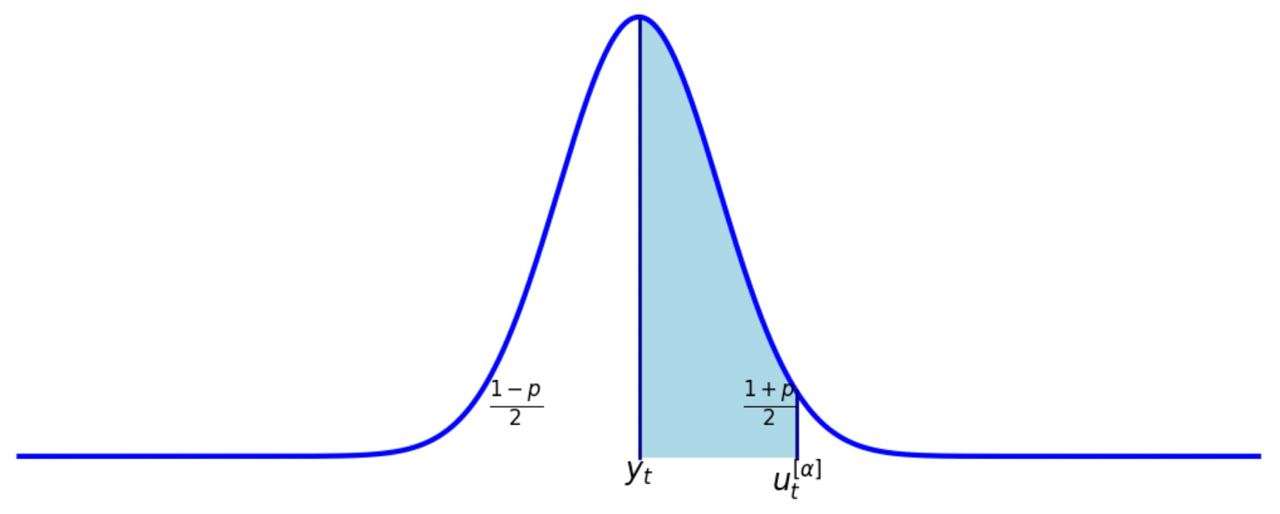
\includegraphics[width=0.8\columnwidth]{figures/kernel_tuning.jpg}}
\label{fig:kernel_tuning_example}
\end{figure}

This approach has many positive points, some of which are worth mentioning:

\begin{itemize}
    \item In terms of importance weights, the posterior particle weights are non-uniform and proportional to the distance between the simulated pseudo-measurements \(u_t^{(i)}\) and the true measurement \(y_t\). The usefulness of this can be seen directly in a resampling step that involves the replication of the particles with a higher probability and removing the ones with negligible weight.
    \item It is also worth highlighting the moment of building a kernel around the true measurement \(y_t\). The benefit of this is that regardless of the initial dispersion of the particles, too high or the opposite too low, eventually, they gradually concentrate around the true value of \(x_t^{(i)}\).
    \item Compared with the same particle filter, it can be said that the process of posterior weights computation differs only in the fact that instead of a true measurement model, the kernel is used, sacrificing performance, but getting more robustness. As it was already possible to understand, the computational complexity of the filter will directly depend on the selected kernel.
\end{itemize}

As one may have understood earlier, the first step of the described steps is nothing other than the standard sorting algorithm. As for the second step, it is not so trivial and involves finding the corresponding value of \(\varepsilon_t\), which is a more complex task that will be considered in detail further.

\paragraph*{Computation of \(\varepsilon_t\)}
Returning to the equation  \(\ref{eq:kernel_tuning}\), it is clear that \(u_t^{[\alpha]}\) is either the \(\frac{1-p}{2}\)-quantile or the \(\frac{1+p}{2}\)-quantile of \(\tilde{g}_{y_t, \varepsilon_t}\left(u_t\right)\) depending on the condition being met: \(u_t^{[\alpha]} \leq y_t\) or \(u_t^{[\alpha]} \geq y_t\). By definition, the quantile function gives the \(\rho\)-quantile. One can easily get around the point of determining if the value of \(u_t^{[\alpha]}\) is greater or less than the true value of \(y_t\) by using a symmetric kernel. In that case, it will be sufficient to consider only the non-negative distance, i.e., the \(\frac{1+p}{2}\)-quantile.

Before disassembling the quantile function, it is necessary to refer to the cumulative distribution function (CDF), the inversion of which is a quantile function. Suppose the F denotes the CDF of the kernel \(\tilde{g}_{0, 1}\left(\cdot\right)\), which, as could be understood, is centered at 0 and with radius 1, then provided the kernel is from the location-scale family, it is possible to obtain a formulation of the quantile function for the kernel in general form \(\tilde{g}_{y_t, \varepsilon_t}\left(\cdot\right)\), which looks as follows:

\begin{equation}
    Q(\rho)=y_t+\varepsilon_t F^{-1}(\rho), \quad \rho \in[0,1].
\end{equation}

Returning to the assumption that the kernel used is symmetric, we can find the desired \(\varepsilon_t\) by substituting \(u_t^{[\alpha]}\) into the previously derived formulation of the quantile function, thereby obtaining the following:

\begin{equation}
    \varepsilon_t=\frac{\left|Q\left(\frac{1+p}{2}\right)-y_t\right|}{F^{-1}\left(\frac{1+p}{2}\right)}=\frac{\left|u_t^{[\alpha]}-y_t\right|}{F^{-1}\left(\frac{1+p}{2}\right)}.
    \label{eq:radius_eq_for_kernel_tuning}
\end{equation}

As can be seen, the numerator of the division is taken as an absolute value, which directly reflects the symmetry property of the kernel. That is why it makes no difference if \(\alpha\)-th closest pseudo-measurement is greater or less than the true value of \(y_t\). So the only parameterized parameters are \(p\) and \(\alpha\).

Now it is time to take a look at some examples of commonly used kernel functions.

\paragraph*{Examples of commonly used kernels} 
This chapter contains a brief examination of the several kernels that are often used in practice, demonstrating the differences between them, as well as deriving rules for using them in the above formula (\ref{eq:radius_eq_for_kernel_tuning}). For more information concerning the information described below, please refer to the works \cite{dedecius_adaptive_2017} and \cite{dedecius_diffusion_2015}.

\begin{itemize}
    \item \textbf{The Gaussian kernel} (alternatively the normal kernel) Assume the standard deviation represented as a positive scale parameter\(\varepsilon_t\) as well as the translation into \(y_t\), then the kernel is given by

    \begin{equation}
        \tilde{g}_{y_t, \varepsilon_t}\left(u_t^{(i)}\right) =  \frac{1}{\sqrt{2 \pi \varepsilon_t^2}} \exp \left\{-\frac{(u_t^{(i)}-y_t)^2}{2 \varepsilon_t^2}\right\} \propto \exp \left(\frac{\left|u_t^{(i)}-y_t\right|^2}{\varepsilon_t^2}\right).
    \end{equation}

    It is worth admitting that this is one of the most frequently used kernel functions. A Gaussian kernel is shaped like a Gaussian (normal distribution) curve. One of the advantages of using the Gaussian kernel can be seen in the example of outliers. When \(y_t\) is an outlier, to prevent the filter from collapsing, the nearly uniform weights are assigned to particles, considering the flat of the kernel. The quantile function of \(\mathcal{N}\left(y_t, \varepsilon_t^2\right)\) has the following form:

    \begin{equation*}
        Q(\rho)=y_t+\varepsilon_t \Phi^{-1}(\rho), \quad \rho \in[0,1],
    \end{equation*}
    
    \noindent where, as already be known, \(\Phi^{-1}\) denotes the quantile of the standard normal distribution, that is, centered at 0 and with a scale equal to 1. That is, the derivation rule \(\varepsilon_t\) for the kernel in general form \(\tilde{g}_{y_t, \varepsilon_t}\left(u_t^{(i)}\right)\) will look as follows:

    \begin{equation}
        \varepsilon_t=\frac{\left|u_t^{[\alpha]}-y_t\right|}{\Phi^{-1}\left(\frac{1+p}{2}\right)}.
        \label{eq:radius_eq_for_kernel_tuning}
    \end{equation}

    \item \textbf{The Cauchy kernel} The same as for the previous one, assume a positive scale parameter as well as the translation into \(y_t\), then the kernel is given by

    \begin{equation}
        \tilde{g}_{y_t, \varepsilon_t}\left(u_t^{(i)}\right) = \frac{1}{\pi \varepsilon_t\left[1+\left(\frac{u_t^{(i)}-y_t}{\varepsilon_t}\right)^2\right]} \propto \left(1+\frac{\left|u_t^{(i)}-y_t\right|^2}{\varepsilon_t^2}\right)^{-1}
    \end{equation}
    In contrast to the previous Gaussian, the Cauchy kernel has more pronounced heavy tails.
    {\em
    "The Cauchy kernel is always centered where relevant peaks of the data are, while the Gaussian kernel tries to accommodate the outliers through an extremely flat component. The Cauchy kernel does not need such a flat component since its heavy tails can deal with the extreme values already."
    } (\cite{kalantan_quantile-based_2019})
    In the case of using the Cauchy kernel, it can be said that the values of weights will much better reflect the closeness of \(u_t^{(i)}\) to the true \(y_t\). And the corresponding quantile function of the \(\mathcal{C}\text{auchy}\left(y_t, \varepsilon_t\right)\) distribution has the following form:

    \begin{equation*}
        Q(\rho) = y_t+\varepsilon_t \underbrace{\tan \left[\pi\left(\rho-\frac{1}{2}\right)\right]}_{\substack{\text{\(F^{-1}(\rho)\)}}} , \quad \rho \in[0,1],
    \end{equation*}
    \noindent where \(F^{-1}\) represents the quantile function of the standard Cauchy distribution. And, accordingly, the required \(\varepsilon_t\) is computed as follows:

    \begin{equation}
        \varepsilon_t=\frac{\left|u_t^{([\alpha])}-y_t\right|}{\tan \left(\frac{\pi p}{2}\right)}
    \end{equation}
        
    \item \textbf{The Uniform kernel} Under all the same conditions as in the previous cases, the kernel has the following form
    \begin{equation}
        \tilde{g}_{y_t, \varepsilon_t}\left(u_t^{(i)}\right) = \begin{cases}\frac{1}{2 \varepsilon_t} & \text { for }-\varepsilon_t \leq u_t^{(i)} - y_t \leq \varepsilon_t \\ 0 & \text { otherwise }\end{cases}.
    \end{equation}
    It is worth noting that such a kernel essentially adheres to the ABC formulation, i.e., only those \(u_t^{(i)}\) that \(u_t \notin A_{\epsilon, y}\) (that is \( \left|u_t^{(i)} - y_t\right| \nleq \epsilon\)) are discarded.

    {\em
    "
    Most of the ABC methods, ie, both static and sequential, adopt a uniform kernel assigning equal weights to particles yielding pseudo-observations within a predefined radius around the true observation and discarding the rest."
    } (\cite{dedecius_marginalized_2018})
    As it can be already concluded, with this approach it is not necessary to compute the \(\varepsilon_t\), the predefined radius is sufficient.
\end{itemize}

All of the above regarding kernels can be summarized by the following visualization (\ref{fig:commonly_used_kernels}):

\begin{figure}[!ht]
\centering
\caption{Visualization of commonly used kernel functions such as Gaussian, Cauchy, and Uniform. The graph shows absolutely all kernels under the same conditions, that is, centered at 0 with a scale equal to 1.3}
\subfloat{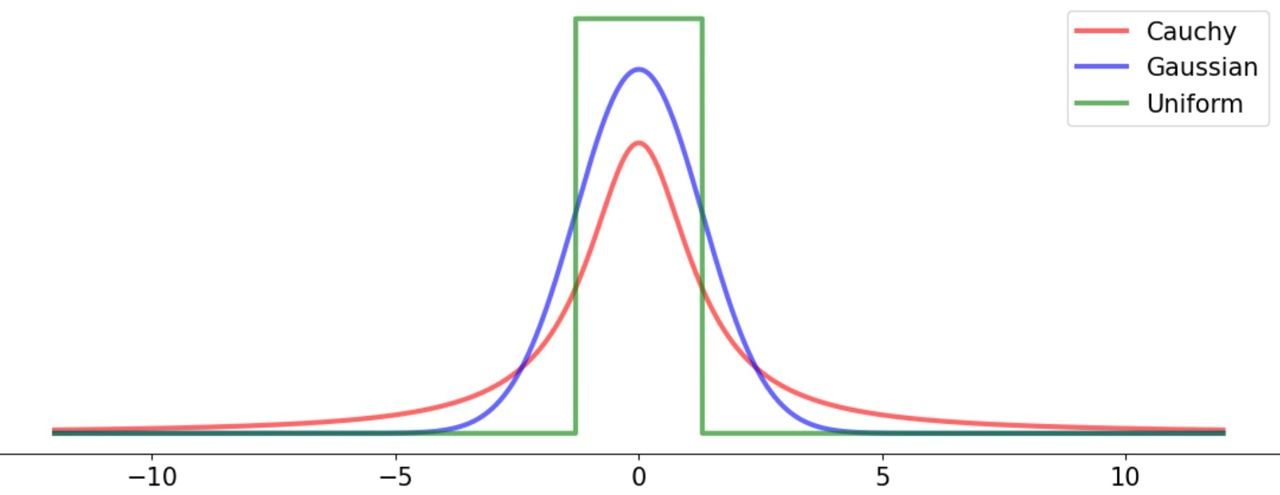
\includegraphics[width=0.9\columnwidth]{figures/commonly_used_kernels.jpg}}
\label{fig:commonly_used_kernels}
\end{figure}

As for increasing the computational complexity, when integrating the technique described above into the algorithm of the usual particle filter, the search step of the \(\alpha\)-th closest pseudo-measurement to true \(y_t\) is added, as well as the subsequent computation of \(\varepsilon_t\). Both described operations are pretty cheap. As stated earlier, the computational complexity depends directly on the chosen kernel function. For example, the calculation of posterior weights can be a cheaper operation when using the Cauchy kernel compared to the particle filter under the condition of the normal measurement model.

\paragraph*{Adaptive kernels in ABC particle filter} 
At this point, all the necessary components have been obtained to approach the problem, which is the key objective of this work, namely, making the inference in the SSMs models with a misspecified or even unknown measurement model. It only remains to bring all of the above theory into a general form and summarize everything with the formulation of the desired algorithm.

The algorithm is based on the already well-known particle filter algorithm, given that the measurement model is not specified as a probability density function \(g\left(y_t \mid x_t^{(i)} \right)\). The ABC approximation will be used instead of the measurement model. Also, unlike the algorithm (\ref{alg:abc_particle_filter}), which used the indicator \(\mathbb{I}_{A_{{\varepsilon_t, y_t}}}\), a more elegant approach through a kernel function will be used. The use of the kernel function will be useful to better reflect the proximity of pseudo-measurements to the true \(y_t\) value by assigning the corresponding weights: the larger weights for pseudo-measurements lying closer to the true \(y_t\) and the smaller ones for those farther away. In addition, automatic kernel scaling at each point in time will be used so that the kernel function is able to cover a sufficient number of pseudo-measurements. The algorithm itself looks as follows (\ref{alg:abc_particle_filter_with_kernel_tuning}):

\begin{algorithm}
    \caption{ABC particle filter with automatic kernel tuning}
  \begin{algorithmic}[1]
    \INPUT \(\{y_1, . . . , y_T\}\), number of particles N, the HPR value \(p\), the number of covered pseudo-measurements \(\alpha\)
    \OUTPUT Estimates \(\{\hat{x}_{0:T}\}\)
    \STATE \textbf{Initialization} Sample \(x_0^{(i)}\) from a suitable a priori distribution \(p(x_0)\) and assign them the initial uniform weights \(w_0^{(i)} = 1/N\).
    \FOR{t = 1,2,...,T}
      \STATE \textbf{Resampling}: Select \(\tilde{x}_{t-1}^{(i)}\sim \sum_{i=1}^N W_{t-1}^{(i)} x_{t-1}^{(i)}\) proportional to their weights \(W_{t-1}^{(i)}\) and reset related all weights \(1/N\).
      \STATE \textbf{Prediction}: Sample N particles from the importance density \(x_t^{(i)} \sim f\left(x_t \mid \tilde{x}_{t-1}^{(i)}\right)\)
      \STATE \textbf{Simulation} Simulate a pseudo-measurements $u_t^{(i)} \sim g\left(y_t \mid x_t^{(i)} \right)$
      \STATE \textbf{Identifying \(u_t^{[\alpha]}\)} Find the \(\alpha\)-th closest pseudo-measurement to \(y_t\)
      \STATE \textbf{Computation of \(\varepsilon_t\)} Calculate kernel scale according to $    \varepsilon_t=\frac{\left|u_t^{[\alpha]}-y_t\right|}{F^{-1}\left(\frac{1+p}{2}\right)}$
      \STATE \textbf{Update}: Recalculate weights according to
      \(w_t^{(i)} \propto \tilde{g}_{y_t, \varepsilon_t}\left(u_t^{(i)}\right) W_{t-1}^{(i)}\) and normalize them \(W_t^{(i)} \leftarrow w_t^{(i)}/\sum_{j=1}^N w_t^{(j)}\).
    \STATE \textbf{Estimation} Estimate of the mean of \(E[x_t|\cdot] = \sum_{i=1}^{N}W_{t}^{(i)} x_t^{(i)}\).
    \ENDFOR
  \end{algorithmic}
  \label{alg:abc_particle_filter_with_kernel_tuning}
\end{algorithm}


%---------------------------------------------------------------
%---------------------------------------------------------------
% Well-specified models experiments
%---------------------------------------------------------------
\chapter{Well-specified models experiments}
\label{chap:well_specified}
%---------------------------------------------------------------

Having already had all the necessary theoretical basis passed, it is time to go directly to the practical part. The experiments will be conducted directly on the three different SSMs described in detail below. Among the models will be both linear and non-linear. Such indicators as efficiency, performance, and robustness of the following algorithms will be compared: KF, EKF, particle filter, and the modification of particle filter with ABC approximation and automatic kernel tuning.

Within the framework of this chapter the experiments will be conducted on well-specified correct models. Also, importantly, one of the main tasks in this chapter is to consider the tracking performance of the approximate filtration with adaptive kernels and how close it is to the performance of a regular particle filter using the correct model.

The mean square error (MSE) will be used as a performance indicator, which is calculated as follows:

\begin{equation}
    \begin{aligned}
        M S E &=\frac{1}{t} \sum_{\tau=1}^t\left(\hat{x}_\tau-x_\tau\right)^2 \\
        &=\frac{1}{t} \sum_{\tau=1}^t\left(\sum_{i=1}^N W_\tau^{(i)} x_\tau^{(i)}-x_\tau\right)^2,
\end{aligned}
\end{equation}

\noindent which is residual sum of squares resulting from comparing the predictions \(\hat{x}_t\) with the ground truth \(x_t\). This is one of the most popular metrics for scoring how close the model's outputs are to ground truth desired values. It is worth recalling that in the case of the ideal model, the MSE value will be zero.

\section{Technical prerequisites}
All of the following experiments were performed on the following laptop computer MacBook Pro (Retina, 15-inch, Mid 2014). All experiments were performed repeatedly to obtain sufficiently representative results, as well as to smooth out, if possible, the technical limitations associated with the computing power and technical limitations of the available device.

As for the experiments themselves and the required dependencies, the programming language Python3.9 and the following dependencies were used:
\begin{itemize}
    \item NumPy v.1.21.3 - primarily for mathematical operations
    \item SciPy v.1.7.1 - in most cases only the \textbf{stats} module containing a huge number of statistical functions
    \item Matplotlib v.3.4.3 - responsible for everything related to visualization
\end{itemize}

\section{Example 1: Power growth model}
The first example should, in fact, prove that the performance of the proposed approximate filter with adaptive kernel should be quite close to the performance of the standard bootstrap particle filter or, on the contrary, disprove this statement. It is worth recalling that unlike particle filters, approximate filters do not require full knowledge of the measurement model, i.e. it is sufficient for them to work with equations without noise terms.

On the agenda is a popular problem rooted in such fields as ecology and epidemiology, referred to as the exponential growth model. But let's consider a slightly modified version of the problem, replacing the exponential function with a exponentiation (power)  and call it the power growth model (PGM). The PGM has the following form:

\begin{equation}
\begin{aligned}
    y_t &= k + \mu_t + \varepsilon_t, \\
    \mu_t &= \mu_{t-1}^{1+\nu_{t-1}} + \xi_t, \\    
    \nu_t &= \rho\nu_{t-1} + \zeta_t,
\label{eq:pgm_equations}
\end{aligned}
\end{equation}

\noindent where \(\rho\in[0,1]\) is the "discounting" factor and \(k\) is the drift. We either know both of these variables or we have to estimate them appropriately. As can be seen, the process is nonlinear and very sensitive to combinations of \(\nu_t\) and \(\mu_t\) values. It is enough to keep the inappropriate combination for a while and the process will explode. 

The next step is to make an appropriate state-space model from the above equations:

\begin{itemize}
    \item State evolution model:

    \begin{equation}
        x_t = \begin{bmatrix} \mu_t \\ \nu_t \end{bmatrix}
        = 
        \begin{bmatrix} \mu_{t-1}^{1+\nu_{t-1}} \\ \rho\nu_{t-1} \end{bmatrix}
        + w_t,
   \end{equation}    
    where
    \begin{equation}
        w_t \sim (0, Q) \quad \text{with} \quad Q = \left[\begin{array}{cc}
            \xi_t^2 & 0 \\
            0 & \zeta_t^2
        \end{array}\right],
   \end{equation}

    \noindent that is nonlinear, will require linearization if the EKF is used.
    \item Measurement model:
    \begin{equation}
        \begin{aligned}
    y_t &= H_t x_t + B_t u_t + \varepsilon_t \\
    &= [1, 0]
    x_t + k + \varepsilon_t.
        \end{aligned}
        \label{eq:pgm_measurement_model}
    \end{equation}

    \noindent which does not require linearization, because it is already linear.
\end{itemize}

Since the EKF is one of the filters used in the experiment, it is necessary to linearize the equation of state, i.e., to determine the derivative of the two-dimensional function \(f\left(\cdot\right)\) - the first vector on the right-hand side:

\begin{equation}
F_t =
\begin{bmatrix}
(\nu_{t-1} + 1) \mu_{t-1}^{\nu_{t-1}} &
\mu_{t-1}^{1+\nu_{t-1}} \ln \mu_{t-1} \\
0 & \rho
\end{bmatrix},
\end{equation}
\noindent that is in the state prediction the \emph{nonlinear equation} will be used to predict \(\hat{x}_t^-\) and the time-varying \emph{matrix} \(F_t\) to predict \(P_t^-\). As for the update step, no linearization is required and the linear measurement equation will be used.

Since this chapter assumes that the model is correct specified, the noise terms belong to the following distributions:

\begin{equation}
\begin{aligned}
\varepsilon_t &\sim \mathcal{N}(0, 10^2), \\
\xi_t &\sim \mathcal{N}(0, 0.1^2), \\
\zeta_t &\sim \mathcal{N}(0, 0.01^2),
\end{aligned}
\end{equation}

\noindent the noise variables \(\varepsilon_t\), \(\xi_t\) and \(\zeta_t\) are independent and identically distributed. It is clear that under the following conditions, there is the  Gaussian measurement model \(g_t\), and also, the measurements \(y_t\) are corrupted by Gaussian noise. It can reasonably be expected that both EKF and PF will perform exceptionally well since all necessary assumptions are met.

It is also important to add that since the second equation (\ref{eq:pgm_equations}) has a mathematical operation with raising a number to a degree, in order to avoid numerical errors during filtering, a couple of mathematical tricks have been added to the function that deals with particle evolution, such as discarding particles that lead to invalid values, etc., thus ensuring that SMC filters work normally. Unfortunately, given the architecture of the EKF filter, which cannot select from many particles, no modifications have been added to it. Thus, one should consider that the EKF filter may generate invalid values on one of the iterations.

\paragraph*{Initialization} The initial parameters are \(x_0=[100,0] \), \(k=2\), \(\rho=0.9\), the length of the series is 500 samples. The EKF filter and three variants of SMC filters were compared. Among the SMC filters are the bootstrap PF, the ABC filter with Gaussian kernel, and the ABC filter with Cauchy kernel. The inference started at the following parameters: the prior state values for EKF are \(x_0 = [0, 100]\) and \(P^{-} = 10 I_{2 \times 2} \), where \(I_{2 \times 2}\) denotes the identity matrix of rank 2. For SMC filters, an initial set of 1000 particles for nonlinear states is randomly sampled from \(\mathcal{N}([100,0],
\begin{bmatrix*}
0.1^2 & 0 \\
0 & 0.01^2
\end{bmatrix*}
) \) and used in all SMC filters. Unlike the PF filter, the ABC filters lack the full knowledge of the measurement model. The ABC filters setting are the HPR value \(p = 0.95\) and covers \(90\%\) of pseudo-measurements. Each SMC filter performs a multinomial resampling at the beginning of each time step. An experiment with 100 independent repetitions was conducted to obtain representative results.

\paragraph*{Charts and analysis}
Accordingly, after 100 experiment runs of all filters, each time on newly generated data, the following results were obtained, presented in the graphs below. Figure \ref{fig:pgm_mse_boxplot_normal} shows the statistics of the final MSE values in the form of box plots. As one would expect, with full knowledge of the measurement model, the EKF and PF filters showed quite acceptable and unambiguously best results among the other filters. It was quite expected that PF would prove to be a fairly stable filter, even it can be seen that its results are slightly, but still better than those of EKF. Just the same, it can be observed that with a sufficient number of particles, the PF is more accurate than the EKF, although computationally more expensive. The stability of the filter can also be proved by the fact that the value from the Table \ref{table:pgm_mse_normal}, which shows the average of final MSE values after 100 experiment runs, is not very different from the median value shown on the box plot. Also, compared to standard approximation methods such as EKF, the PF's main advantage is that it does not rely on any local linearization technique. As for ABC filters, it can be stated that their results against the background of EKF and PF look worse, but not much, especially given the lack of accurate knowledge of the measurement model. It can be seen that the ABC filter operation in the context of this model is not quite sensitive to the choice of kernel. So, for example, from Figure \ref{fig:pgm_mse_boxplot_normal}, one can see that the ABC filter with the normal kernel performed slightly better for tracking both state variables \(\mu\) and \(\nu\). Also, if one looks at the table \ref{table:pgm_mse_normal} with the averaged values after all 100 experiment runs, one can observe the same, that the results are almost identical for both ABC filters, but still, the filter with the normal kernel shows a slightly better performance.

\begin{figure}[!ht]
\centering
\caption{(PGM, Normal noise) Box plots showing final MSE values for both state variables \(\mu\) and \(\nu\) of 100 repeated experiments. The boxes show medians, upper and lower quartiles. The length of the whiskers is defined as 1.5 times the interquartile range. The outliers are not displayed.}
\subfloat{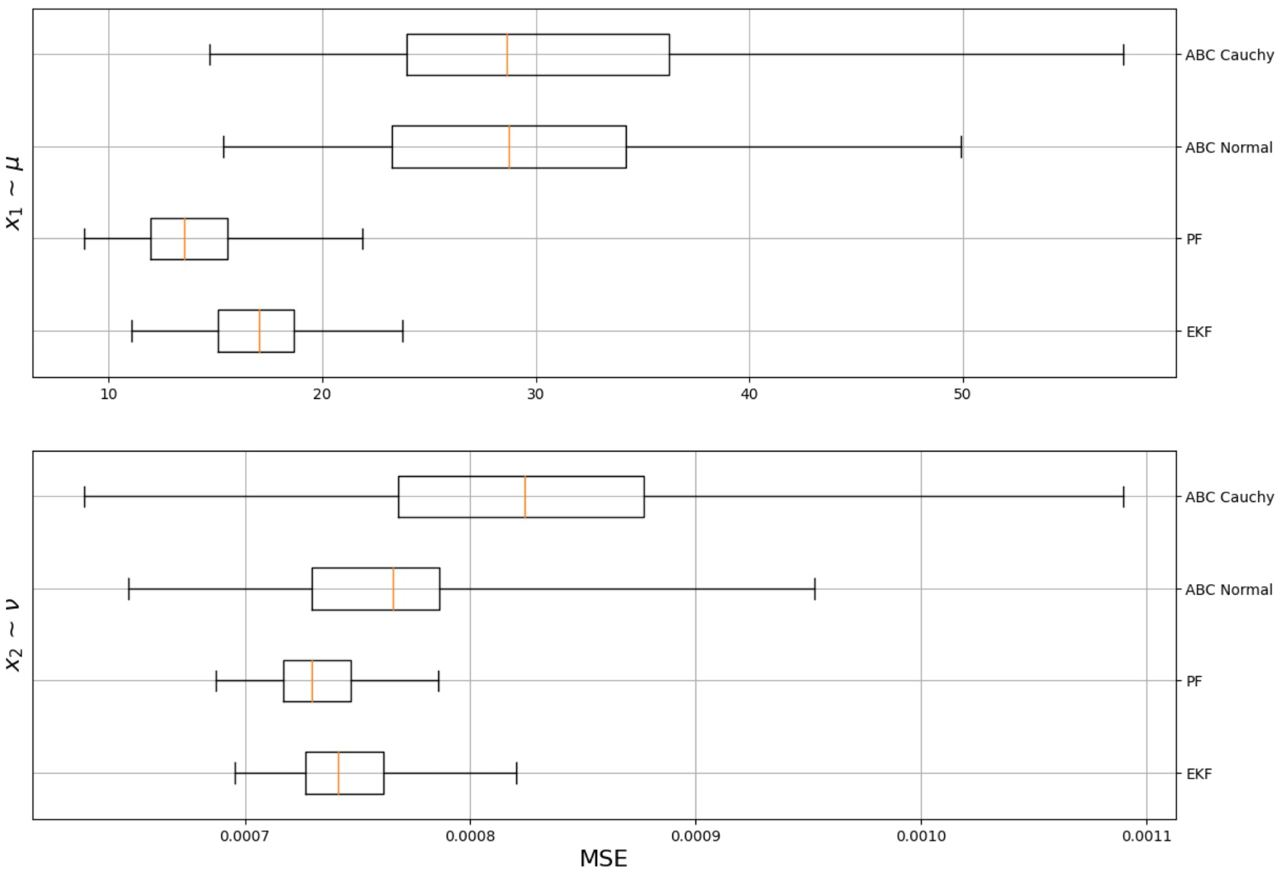
\includegraphics[width=0.9\columnwidth, height=\textheight,keepaspectratio]{figures/pgm/mse_boxplot_normal.jpg}}
\label{fig:pgm_mse_boxplot_normal}
\end{figure}

\begin{table}[h!]
\centering
\begin{tabular}{ |p{4cm}|p{4cm}|p{4cm}|}
 \hline 
  & \(\mu\) & \(\nu\)\\
 \hline \hline
 EKF & 17.029    & 7.435e-04  \\
 PF  &   13.840  & 7.319e-04 \\
 ABC Normal & 29.347 & 7.646e-04\\
 ABC Cauchy & 30.963 & 8.274e-04\\
 \hline
\end{tabular}
\caption{(PGM, Normal noise) The final MSE values for both state variables \(\mu\) and \(\nu\) averaged over 100 runs}
\label{table:pgm_mse_normal}
\end{table}

Another indicator worth paying attention to is shown in Figures \ref{fig:pgm_measurement_noise_normal} and \ref{fig:pgm_abc_scales_evolution_normal}. The first Figure shows the implementation of the measurement noise \(\varepsilon_t\) in the final experiment run, and the second shows the scale settings of the ABC filter kernels in the final experiment run. Basically, both cases show the same \(\varepsilon_t\) evolution characteristics. Clearly, there are some minimal differences, but this is a property of the kernels themselves.


\begin{figure}[!ht]
\centering
\caption{(PGM, Normal noise) One particular normal noise realization \(\varepsilon_t\). Relative frequency histogram and box plot. The box shows the median, upper and lower quartiles. The length of the whiskers is defined as 1.5 times the interquartile range. Dots closer to the edges of the box represent outliers.}
\subfloat{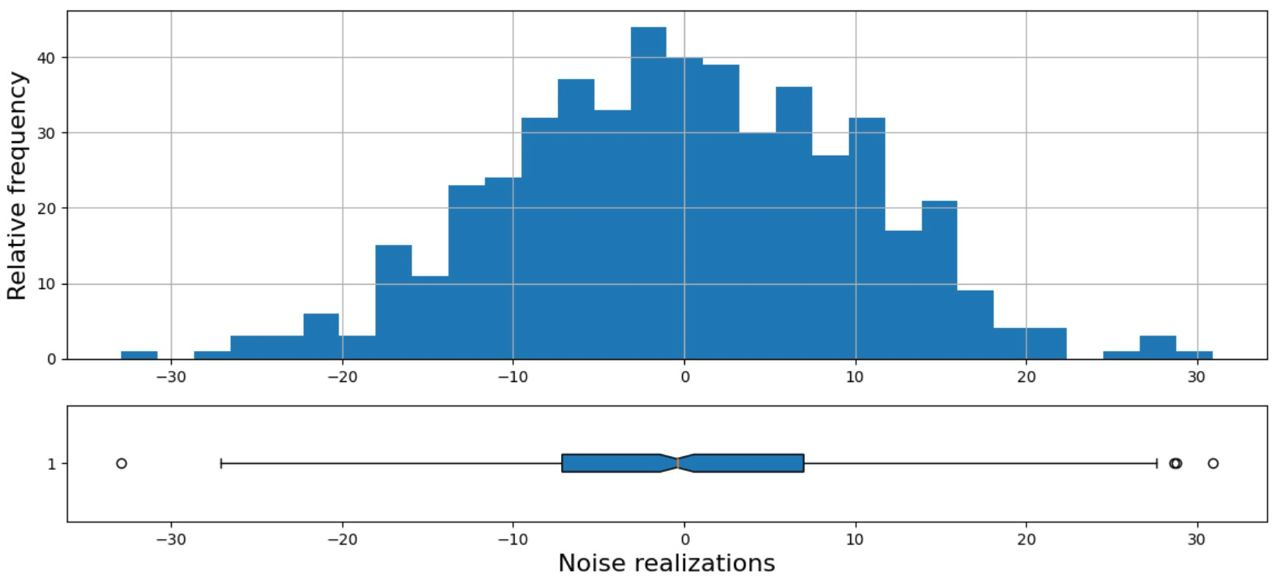
\includegraphics[width=0.9\columnwidth, height=\textheight,keepaspectratio]{figures/pgm/measurement_noise_normal.jpg}}
\label{fig:pgm_measurement_noise_normal}
\end{figure}

\begin{figure}[!ht]
\centering
\caption{(PGM, Normal noise) The top two graphs show the one particular evolution of the normal and Cauchy scales \(\varepsilon_t\), respectively. The bottom one represents the normal noise realizations.}
\subfloat{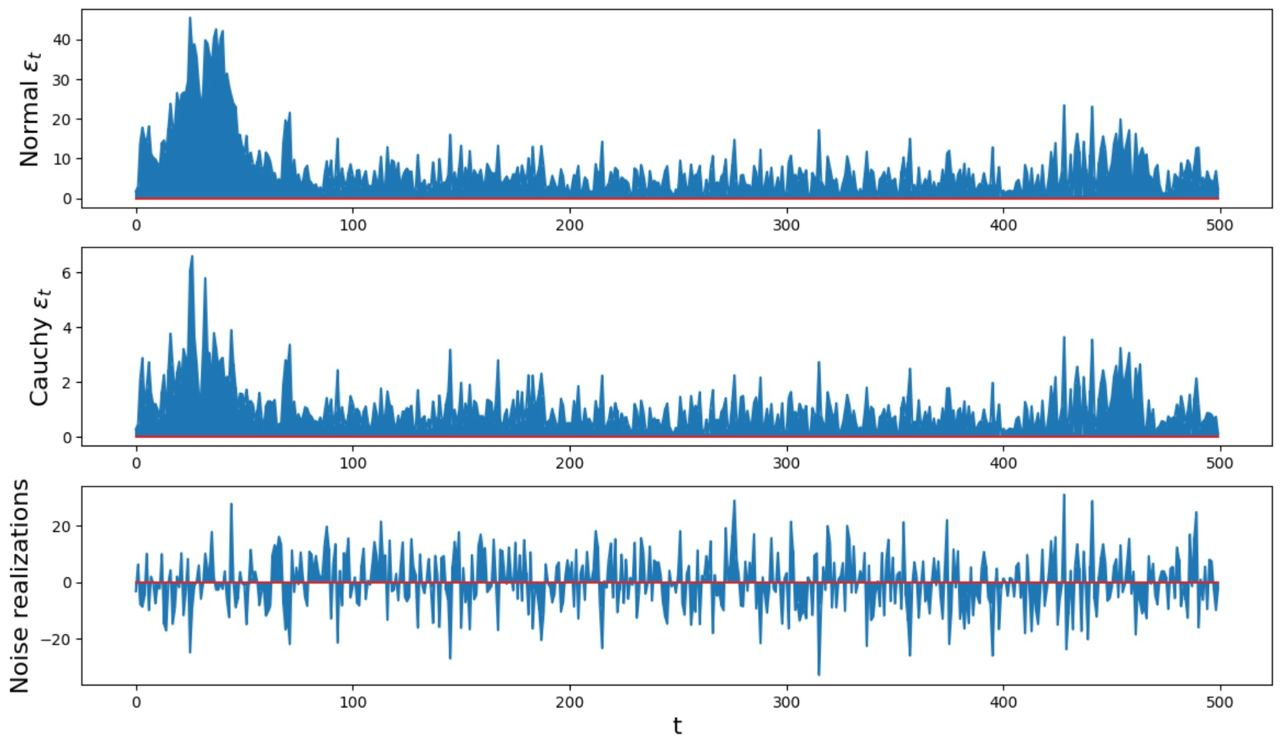
\includegraphics[width=0.9\columnwidth, height=\textheight,keepaspectratio]{figures/pgm/abc_scales_evolution_normal.jpg}}
\label{fig:pgm_abc_scales_evolution_normal}
\end{figure}

In general, based on the example of this experiment, one can say that all the filters showed pretty good results with the obvious favorites. Considering that ABC filters do not require the measurement generating model to be probabilistic, also showed good results. In this example, the ABC filter with the normal kernel stands out slightly better, but overall, both ABC filters showed almost identical good results.

\section{Example 2: Constant velocity model}
Next in line is a fairly popular and well known constant velicty model (CVM). The model is absolutely linear and its purpose is to filter the position of an object moving on the surface, i.e. in 2D. The CVM has the following form:

\begin{equation}
    \begin{aligned}
        x_{1,t} &= x_{1,t-1} + v_{x_1,t} dt + w_{x_1,t}, \\
        v_{x_1,t} &= v_{x_1, t-1} + w_{vx_1, t},
    \end{aligned}
    \label{eq:cvm_equations}
\end{equation}

\noindent where the first equation characterizes the current position of the object in both axes, and the second equation characterizes the velocity of the object at a given time. Consider that the velocity is the same and its changes are caused only by noise. Only position measurements in both axes are available in 1 second time steps. An example for one axis looks like this:

\begin{equation}
\begin{aligned}
    y_{1,t} &= x_{1,t} + \varepsilon_{y_1,t}.
\end{aligned}
\label{eq:cvm_measurement_equation}
\end{equation}

All the same filters will be used for this model as for the previous one, except that this model is absolutely linear, so KF will be used instead of EKF. It is time to make the appropriate SSM from the above equations:

\begin{itemize}
    \item State evolution model:
    
    \begin{equation}
        x_t = \begin{bmatrix}
        x_{1,t} \\ 
        x_{2,t} \\ 
        v_{x_1,t} \\ 
        v_{x_2,t}
\end{bmatrix}
        = \begin{bmatrix}
       1 & 0 & dt & 0 \\
       0 & 1 & 0 & dt \\
       0 & 0 & 1 &  0 \\
       0 & 0 & 0 &  1 
    \end{bmatrix} x_{t-1} + w_t,
   \end{equation}   
   
    \noident where

    \begin{equation}
        w_t \sim (0, Q_t) \quad \text{with} \quad Q = q^2 \cdot
    \begin{bmatrix}
        \frac{dt^3}{3}    & 0                 & \frac{dt^{2}}{2}  & 0  \\
        0                 & \frac{dt^3}{3}    & 0                 & \frac{dt^{2}}{2} \\
        \frac{dt^{2}}{2}  & 0                 & dt                & 0 \\
        0                 & \frac{dt^{2}}{2}  & 0                 & dt
    \end{bmatrix}.
   \end{equation}

   \item Measurement model:

    \begin{equation}
    \begin{aligned}
    y_t &=  \begin{bmatrix}
        1 & 0 &0 & 0 \\
        0 & 1 &0 & 0
    \end{bmatrix} x_t + \varepsilon_t,
        \end{aligned}
        \label{eq:cvm_measurement_model}
    \end{equation}
    \noident where
    \begin{equation}
        \varepsilon_t \sim (0, R_t) \quad \text{with} \quad R =
    r^{2}\cdot
    \begin{bmatrix}
        1 & 0 \\
        0 & 1
    \end{bmatrix}.
   \end{equation}
    
\end{itemize}

Just like last time, based on the assumption that the model is correctly specified, the noise terms belong to following normal distributions:

\begin{equation}
\begin{aligned}
w_t &\sim \mathcal{N}(0, Q_t), \\
\varepsilon_t &\sim \mathcal{N}(0, R_t).
\end{aligned}
\end{equation}

\paragraph*{Initialization} The initial parameters are \(x_0=[0,0,1,-1] \), \(dt=1\), \(r=3\), \(q=\sqrt{5}\), the length of the series is 300 samples. Accordingly, the KF filter and three other variations of SMC filters will be compared. Just like in the previous example, the SMC filters include bootstrap PF and two ABC filters with normal and Cauchy kernels. The initial parameters for the KF filter are \(x_0 = [1,1,1,1]\) and \(P^{-} = 10000 I_{4 \times 4} \). As for the SMC filters, the following setup is provided: an initial set of 1000 particles is randomly sampled from \(\mathcal{N}\left(\left[1,1,1,1\right], 10 I_{4 \times 4} \right)\) and used in all SMC filters. For the ABC filters, the same settings are left as in the previous example: the HPR value \(p = 0.95\) in order to cover \(90\%\) of pseudo-measurements. An experiment with 100 repetitions was conducted to obtain representative results.

\paragraph*{Charts and analysis} 
To begin with, it is worth taking a look at the statistics of the final MSE values. Figure \ref{fig:cvm_mse_boxplot_normal} presents the statistics of the final MSE values of 100 repeated experiment runs in form of box plots. The table \ref{table:cvm_mse_normal} shows the averaged MSE values after 100 experiment runs for all filters used.

According to the results in Figure \ref{fig:cvm_mse_boxplot_normal}, it can again state that globally the KF and PF filters succeeded best in tracking all 4 state variables. As it is already known from theoretical part that KF is the best possible linear estimator, and this is confirmed in this example, because it showed excellent results. Almost identical, but a little worse results were shown by PF, although it succeeded a little better with tracking \(v_2\). The ABC filters also showed good results in tracking state variables. According to box plots, it may seem that ABC filter with normal kernel performs better than similar filter with Cauchy kernel. Given that the ABC filter with Cauchy kernel has the most distant right whisker, i.e., the maximum error value, it can be concluded that, despite the good performance, it still sometimes made quite strong errors compared to the others. 
But if we look at the average of the final values for all experiment runs in the Table \ref{table:cvm_mse_normal}, one can see that the final averaged MSE values of both ABC filters are quite close. But it should admitted that the results of the filter with the normal kernel are slightly, but still better.

\begin{figure}[!ht]
\centering
\caption{(CVM, Normal noise) Box plots showing final MSE values for all state variables $x_1$, $x_2$, $v_1$ and $v_2$ of 100 repeated experiments. The boxes show medians, upper and lower quartiles. The length of the whiskers is defined as 1.5 times the interquartile range. The outliers are not displayed.}
\subfloat{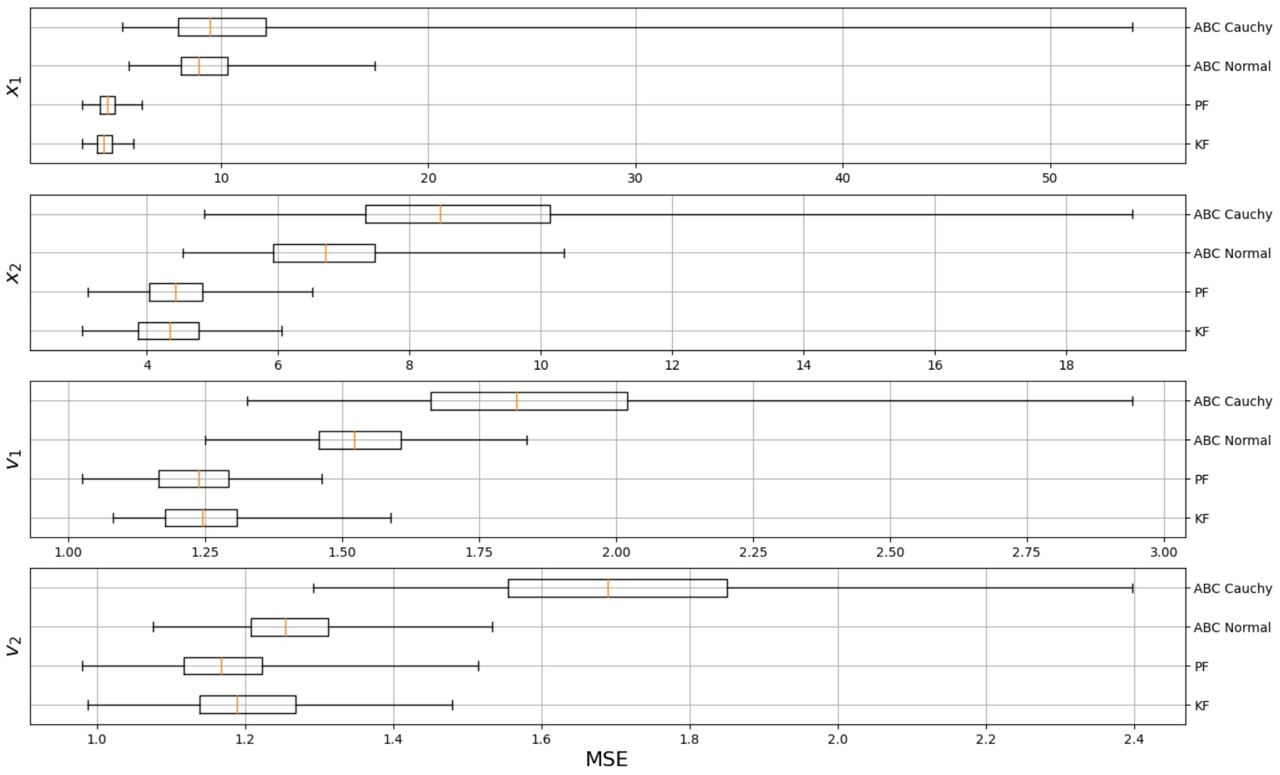
\includegraphics[width=0.9\columnwidth, height=\textheight,keepaspectratio]{figures/cvm/mse_boxplot_normal.jpg}}
\label{fig:cvm_mse_boxplot_normal}
\end{figure}

\begin{table}[h!]
\centering
\begin{tabular}{ |p{2cm}|p{2cm}|p{2cm}|p{2cm}|p{2cm}|}
 \hline 
  & $x_1$ & $x_2$ & $v_1$ & $v_2$ \\
 \hline \hline
 KF & 4.405 & 4.364 & 1.253 & 1.202  \\
 PF & 4.531 & 4.450 & 1.235 & 1.176 \\
 ABC Normal & 9.256 & 6.783 & 1.534 & 1.263 \\
 ABC Cauchy & 11.363 & 9.013 & 1.869 & 1.717 \\
 \hline
\end{tabular}
\caption{(CVM, Normal noise) The final MSE values for all state variables $x_1$, $x_2$, $v_1$ and $v_2$ averaged over 100 runs}
\label{table:cvm_mse_normal}
\end{table}

In general, however, it can be noted that both ABC filters were quite close to reality in their predictions. Proof of this can be found in Figures \ref{fig:cvm_measurement_noise_normal} and \ref{fig:cvm_abc_scales_evolution_normal}, which show one particular realization of measurement noises \(\varepsilon_{y_1,t}\) and \(\varepsilon_{y_2,t}\), and also the resulting settings of kernels. Once again, as in the previous example, the ABC filter in this model is not overly sensitive to kernel choice. As for kernel tuning, one can see that the character of the evolution of both \(\varepsilon_{y_1,t}\) and \(\varepsilon_{y_2,t}\) is similar for both kernels. It is impossible to find any significant differences.

\begin{figure}[!ht]
\centering
\caption{(CVM, Normal noise) One particular normal noise realizations \(\varepsilon_{y_1,t}\) and \(\varepsilon_{y_2,t}\). Relative frequency histograms and box plots. Each box shows the median, upper and lower quartiles. The length of the whiskers is defined as 1.5 times the interquartile range. Dots closer to the edges of the box represent outliers.}
\subfloat{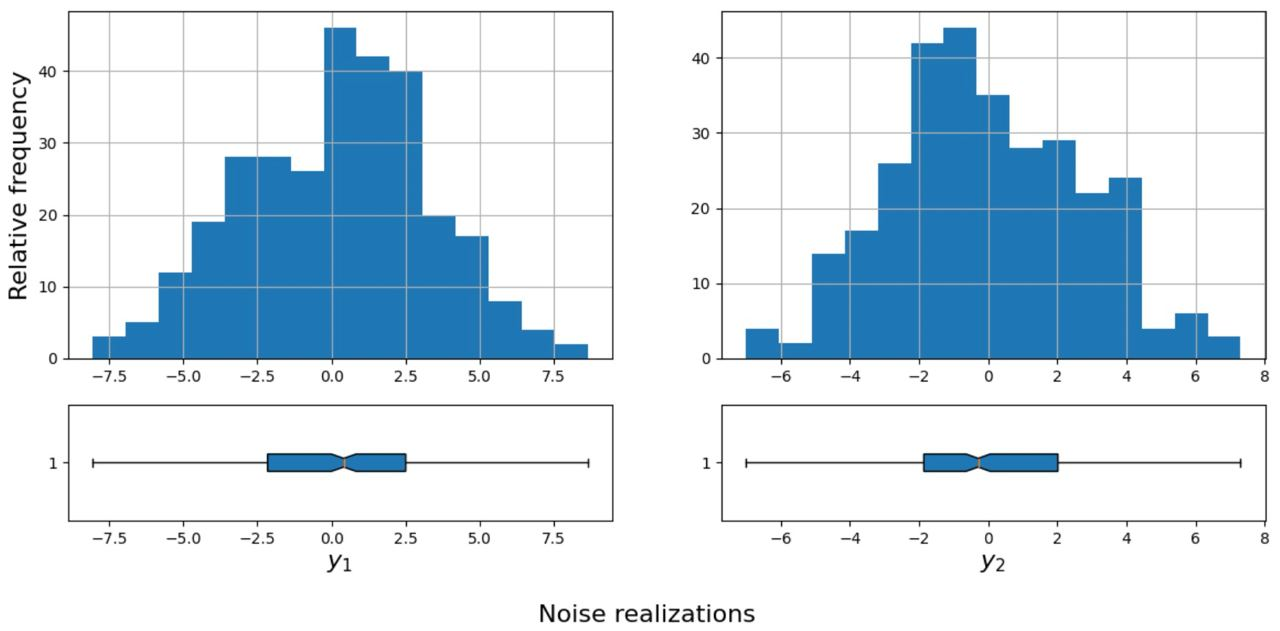
\includegraphics[width=0.9\columnwidth, height=\textheight,keepaspectratio]{figures/cvm/measurement_noise_normal.jpg}}
\label{fig:cvm_measurement_noise_normal}
\end{figure}

\begin{figure}[!ht]
\centering
\caption{(CVM, Normal noise) The top four graphs show the one particular evolution of the normal and Cauchy scales \(\varepsilon_{y_1,t}, \varepsilon_{y_2,t}\), respectively. The bottom two represent the normal noise realizations.}
\subfloat{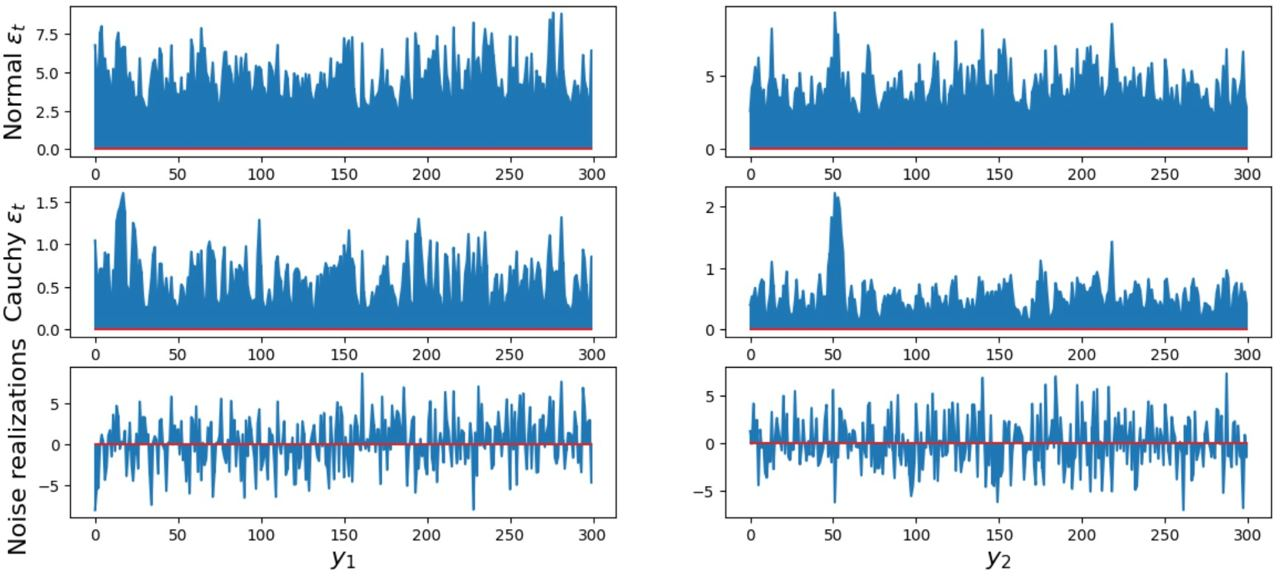
\includegraphics[width=0.9\columnwidth, height=\textheight,keepaspectratio]{figures/cvm/abc_scales_evolution_normal.jpg}}
\label{fig:cvm_abc_scales_evolution_normal}
\end{figure}

Again, as in the case of the PGM model, it can be argued that ABC filters can compete with filters requiring full knowledge of the measurement model, provided that these filters possess such knowledge. Given the context of full knowledge of the measurement model, it is still better to use KF, since of all the filters used in the experiment, it is the cheapest in terms of computational cost and the most accurate in terms of tracking.

\section{Example 3: Polar radar model}
The model that will be presented in this section is a modification of the CVM model, adding nonlinearity to it. Again, there is an object moving in 2D space, accurately described by equations (\ref{eq:cvm_equations}). But here it is assumed that the measurements of the object's motion will come directly from the radar. That is, in the context of this model, the measurements will be represented in a Polar coordinate system. 

The state evolution model, its noise term, and the corresponding covariance matrix remain identical to the CVM. As for the measurement model, it will look like this:

\begin{equation}
    \begin{aligned}
     y_t &=
    \begin{bmatrix}
        \rho_t \\ 
        \phi_t \\ 
        \dot{\rho}_t
    \end{bmatrix}
    = h(x_{t}) + \varepsilon_t,
    \end{aligned}
    \label{eq:prm_equations}
\end{equation}

\noident where

\begin{equation}
    \varepsilon_t \sim (0, R_t) \quad \text{with} \quad R &=
    r^{2}\cdot
    \begin{bmatrix}
        0.01 & 0.0 & 0.0 \\
        0.0 & 0.0001 & 0.0 \\
        0.0 & 0.0 & 0.01
    \end{bmatrix}.
\end{equation}

Where respectively the measurement \(y_t\) is a polar coordinate, which consists of the following elements: \(\rho\), \(\dot{\rho}\) are radius and velocity magnitude respectively and \(\phi\) is the angle in radians. Also, it was already clear that the function \(h(\cdot)\) is the function that converts 2D Cartesian position and velocity coordinates to Polar coordinates. This function is necessary because the prediction will be in Cartesian coordinates, but the measurement that comes from the radar is in Polar coordinates. The function itself looks as follows:

\begin{equation}
h\left(x\right)=\left(\begin{array}{c}
\rho \\
\phi \\
\dot{\rho}
\end{array}\right)=\left(\begin{array}{c}
\sqrt{x_1^2+x_2^2} \\
\arctan \left(x_2 / x_1\right) \\
\frac{x_1 v_1+x_2 v_2}{\sqrt{x_1^2+x_2^2}}
\end{array}\right).
\end{equation}

The set of filters that will take part in the experiment is already standard. Because of the use of the conversion function in the measurement equation, which is clearly non-linear, instead of the usual KF filter will be used its extended version. To use EKF in the measurement update cycle, one must linearize the function \(h(\cdot)\), that is, use a Taylor series expansion and take its first derivative. Since the work in the equation is done with a matrix, one can easily calculate its first-order derivative using the Jacobian matrix. That is, the linearization for the correction will look as follows:

\begin{equation}
    H = h'(x) = \left[\begin{array}{cccc}
\frac{x_1}{\sqrt{x_1^2+x_2^2}} & \frac{x_2}{\sqrt{x_1^2+x_2^2}} & 0 & 0 \\
-\frac{x_2}{x_1^2+x_2^2} & \frac{x_1}{x_1^2+x_2^2} & 0 & 0 \\
\frac{x_2\left(v_1 x_2-v_2 x_1\right)}{\left(x_1^2+x_2^2\right)^{3 / 2}} & \frac{x_1\left(v_2 x_1-v_1 x_2\right)}{\left(x_1^2+x_2^2\right)^{3 / 2}} & \frac{x_1}{\sqrt{x_1^2+x_2^2}} & \frac{x_2}{\sqrt{x_1^2+x_2^2}}
\end{array}\right]
\end{equation}

And as in the previous examples in this chapter, based on the assumption that the model is correctly specified, the noise terms belong to following normal distributions:

\begin{equation}
\begin{aligned}
w_t &\sim \mathcal{N}(0, Q_t), \\
\varepsilon_t &\sim \mathcal{N}(0, R_t).
\end{aligned}
\end{equation}

\paragraph*{Initialization} The model initialization parameters will not differ from what was set in the CVM. The initial parameters are \(x_0=[0,0,1,-1] \), \(dt=1\), \(r=3\), \(q=\sqrt{5}\), the length of the series is 300 samples. As for the EKF filter: \(x_0 = [1,1,1,1]\) and \(P^{-} = 10000 I_{4 \times 4}\). An initial set of 1000 particles is randomly sampled from \(\mathcal{N}\left(\left[1,1,1,1\right], 10 I_{4 \times 4} \right)\) and used in all SMC filters. The setting of the ABC filters also remain unchanged from previous experiments: the HPR value \(p = 0.95\) in order to cover \(90\%\) of pseudo-measurements. An experiment with 100 repetitions was conducted to obtain representative results.

\paragraph*{Charts and analysis}
The analysis will begin again with a consideration of MSE values, which are represented by Figure \ref{fig:pgm_mse_boxplot_normal} and Table \ref{table:prm_mse_normal}, where the first figure shows the final results after 100 experiment runs and the second figure shows the averaged values. Also with regard to box plots, for better readability and because of the longest whiskers, the results for the ABC filter with Cauchy kernel for the state variables \(x_1\) and \(x_2\) are put on a separate graph (in the middle).

Given the rather high non-linearity of the measurement model, almost all filters showed far from outstanding results, especially when it comes to tracking \(x_1\) and \(x_2\). The best of all were, as throughout this chapter, the EKF and PF filters. This time the PF filter performed worse than the EKF. From the Figure \ref{fig:pgm_mse_boxplot_normal} with box plots, one can see that PF was sometimes very inaccurate when tracking \(x_1\) and \(x_2\). This is also confirmed by the Table \ref{table:prm_mse_normal} with averaged values. As for the ABC filters, they in particular experienced great difficulty in keeping track of the state variables \(x_1\) and \(x_2\). The final MSE values of some experiment runs were so high that they also affected the averaged values in the Table \ref{table:prm_mse_normal}. If ABC with a normal kernel has a critical averaged MSE value only when tracking the variable \(x_1\), then a filter with a Cauchy kernel has a huge averaged MSE for both \(x_1\) and \(x_2\). As for tracking \(v_1\) and \(v_2\), all filters showed generally acceptable results. Returning to the ABC filters, it can be said that this time they did not prove to be competitive, especially the filter with the Cauchy kernel showed the worst results.

\begin{figure}[!ht]
\centering
\caption{(PRM, Normal noise) Box plots showing final MSE values for all state variables $x_1$, $x_2$, $v_1$ and $v_2$ of 100 repeated experiments. The boxes show medians, upper and lower quartiles. The length of the whiskers is defined as 1.5 times the interquartile range. The outliers are not displayed.}
\subfloat{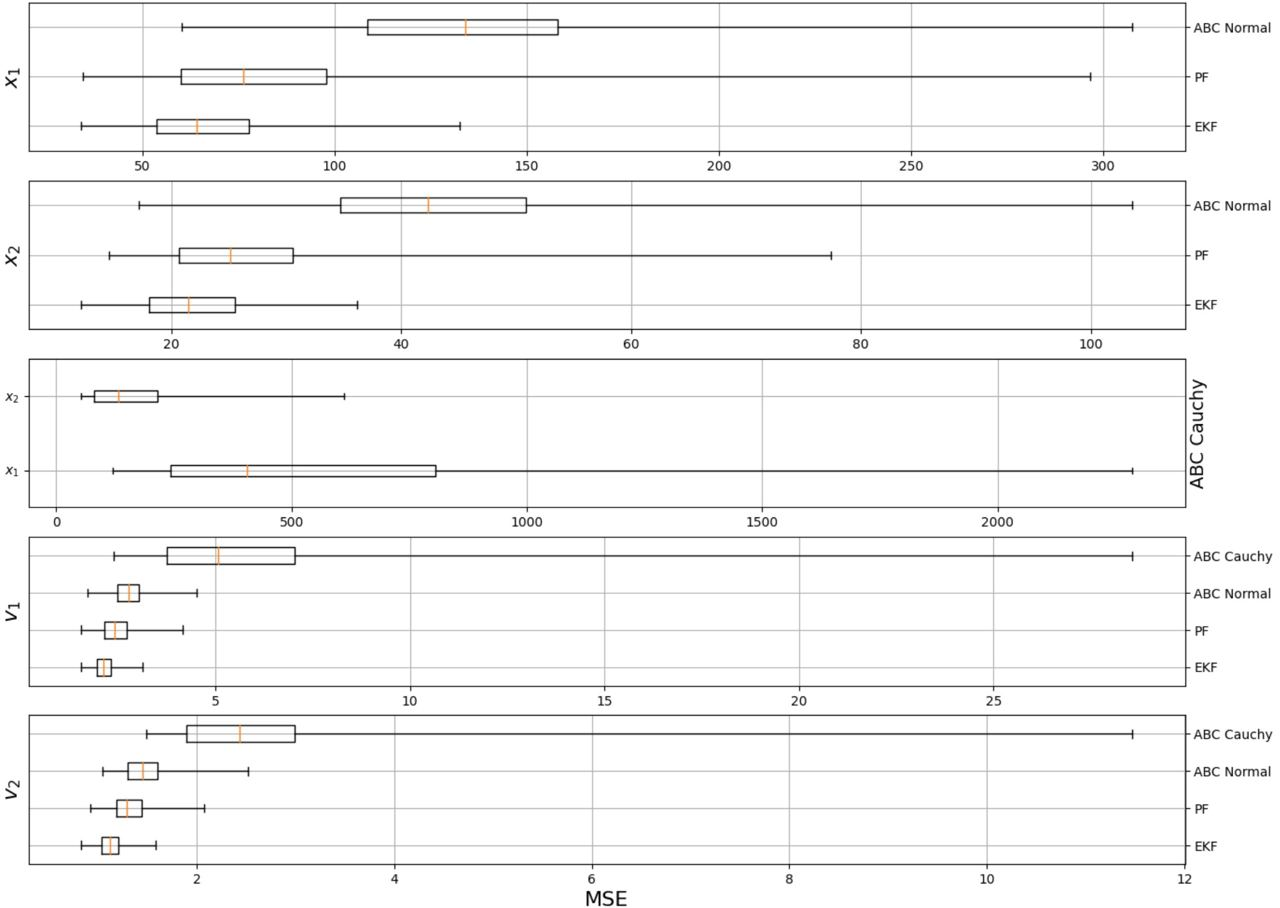
\includegraphics[width=0.9\columnwidth, height=\textheight,keepaspectratio]{figures/prm/mse_boxplot_normal.jpg}}
\label{fig:prm_mse_boxplot_normal}
\end{figure}

\begin{table}[h!]
\centering
\begin{tabular}{ |p{2cm}|p{2cm}|p{2cm}|p{2cm}|p{2cm}|}
 \hline 
  & $x_1$ & $x_2$ & $v_1$ & $v_2$ \\
 \hline \hline
 EKF & 66.235 & 21.636 & 2.161 & 1.122  \\
 PF & 81.980  & 26.763 & 2.433 & 1.333 \\
 ABC Normal & 140.496 & 44.511 & 2.846 & 1.474 \\
 ABC Cauchy & 957.038 & 261.612 & 5.908 & 2.703 \\
 \hline
\end{tabular}
\caption{(PRM, Normal noise) The final MSE values for all state variables $x_1$, $x_2$, $v_1$ and $v_2$ averaged over 100 runs}
\label{table:prm_mse_normal}
\end{table}

Also on the Figures \ref{fig:prm_measurement_noise_normal} and \ref{fig:prm_abc_scales_evolution_normal}, one can take a closer look at one particular realization of measurement noises \(\varepsilon_{y_1,t}\), \(\varepsilon_{y_2,t}\), \(\varepsilon_{y_3,t}\), and also the resulting settings of kernels. In terms of kernel tuning, on the example of these data it can be stated that the ABC filters reflects well the noise evolution. It is worth expecting that the responses to significant values of the noise terms will be more evident in the next chapter.

\begin{figure}[!ht]
\centering
\caption{(PRM, Normal noise) One particular normal noise realizations \(\varepsilon_{y_1,t}\), \(\varepsilon_{y_2,t}\) and \(\varepsilon_{y_3,t}\). Relative frequency histograms and box plots. Each box shows the median, upper and lower quartiles. The length of
the whiskers is defined as 1.5 times the interquartile range. Dots closer to the edges of the box represent
outliers.}
\subfloat{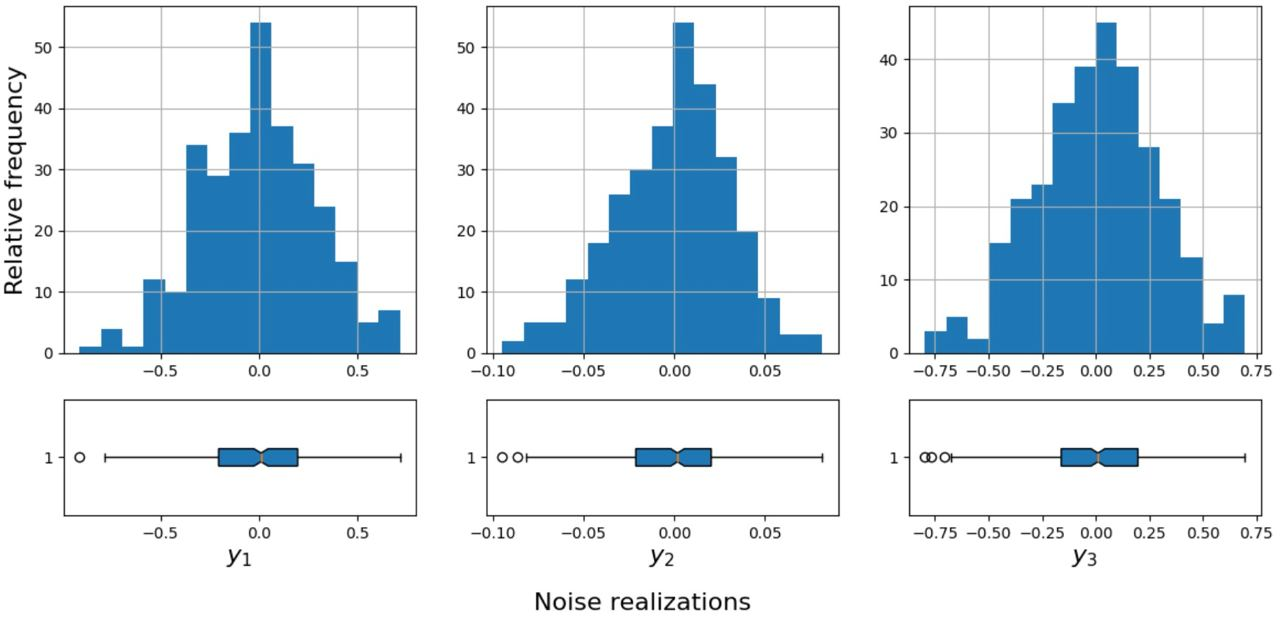
\includegraphics[width=0.9\columnwidth, height=\textheight,keepaspectratio]{figures/prm/measurement_noise_normal.jpg}}
\label{fig:prm_measurement_noise_normal}
\end{figure}

\begin{figure}[!ht]
\centering
\caption{(PRM, Normal noise) The top four graphs show the one particular evolution of the normal and Cauchy scales \(\varepsilon_{y_1,t}, \varepsilon_{y_2,t}\), and \(\varepsilon_{y_3,t}\), respectively. The bottom three represent the normal noise realizations.}
\subfloat{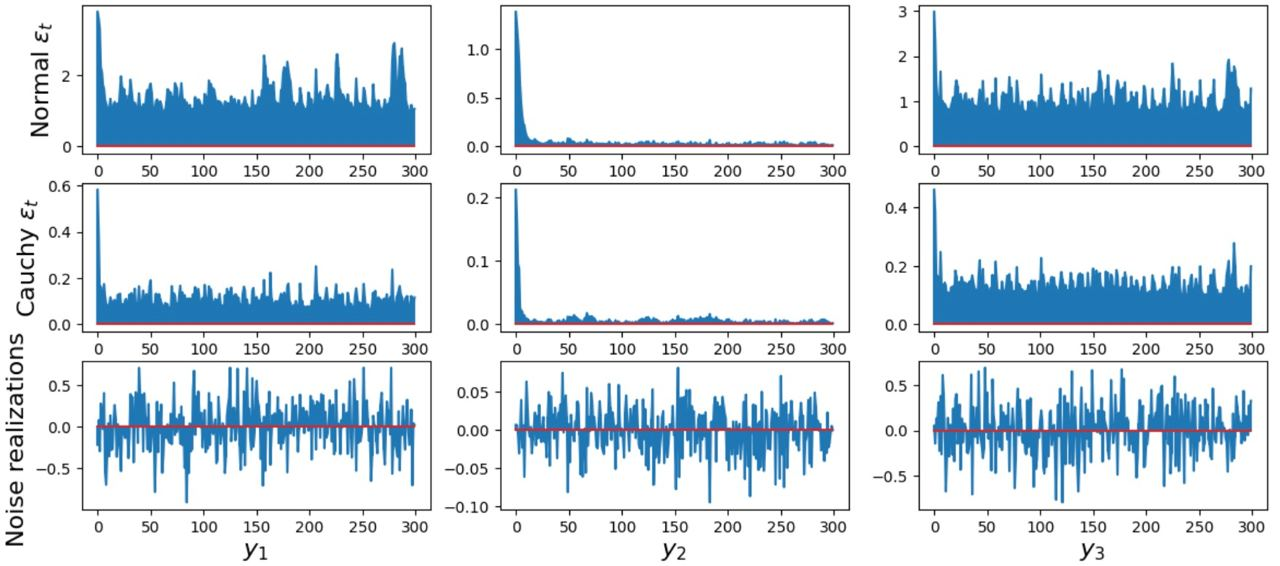
\includegraphics[width=0.9\columnwidth, height=\textheight,keepaspectratio]{figures/prm/abc_scales_evolution_normal.jpg}}
\label{fig:prm_abc_scales_evolution_normal}
\end{figure}

\section{Experiments conclusion}
In general, it can be summarized that with full knowledge of the measurement model, it does not make much sense to use ABC filters, which, in most cases, show pretty good results but are still inferior to PF and KF filters. It is also worth considering that in terms of computational cost, they are insignificantly but still more expensive.

As for the KF filter, having a well-specified model and guaranteed linearity, it can be safely declared that it is the best linear estimator, which is confirmed by the results of the experiments. Its extended version also showed itself from the best side. The PF filter showed itself almost on par with KF and EKF, and sometimes EKF was even inferior to it. However, it should be kept in mind that to use PF, which performs on par or even better than KF or EKF, one will have to sacrifice the use of a large number of particles, which directly affects the computational complexity. It is also worth noting that in the case of EKF, when one of the steps, either prediction or update, is highly nonlinear, EKF will have relatively not the best efficiency. In addition, the quite high computational cost of computing the Jacobian matrix is worth considering when using EKF.

To summarize, once again, it can be said that, if the condition that the measurement model is completely known and both state and measurement equations are linear with zero mean Gaussian noise is satisfied, then it is best to use the standard KF filter. In the case of nonlinearity, it would be better to use the PF filter.
%---------------------------------------------------------------
%---------------------------------------------------------------
% Misspecified models experiments
%---------------------------------------------------------------
\chapter{Misspecified models experiments}
\label{chap:misspecified}
%---------------------------------------------------------------

The purpose of this chapter is to illustrate how the tracking performance of the filters will change if the noise of the measurement model is misspecified or even unknown. The main question and interest is how much better the ABC filters will show themselves under these conditions compared to the others. It is important to remember that the ABC filters ignore the properties of measurement noise, which make them suitable for use directly in such situations, as opposed to the standard PF or KF (or its extended version), where modifications are usually required without much guarantee of success unless laborious tuning is done.

To keep the experiments honest, the same models as in the previous chapter will be used, with the same structure, except that the measurement noise will be Cauchy distributed. At the same time, it will be interesting to see the results of tracking KF and its extended version since they require both state and measurement noises te be Gaussian for optimality. If the first condition remains, the measurement noise in this chapter will use Cauchy distributed, which should already complicate the tracking performance of KFs. KF is expected to work normally for most noise distributions as long as the errors have a zero mean and the distributions are symmetric around the mean. But it will no longer be optimal under Cauchy noise conditions.

The metric for measuring performance in this chapter will remain the same, that is, MSE will be used. The same filters as in the previous chapter will take part in the experiments: the PF, ABC filters with normal and Cauchy kernels, as well as the Kalman filter for linear models and its extended version for nonlinear models.

\section{Example 1: Power growth model}
It is the turn to return to the model described in detail in the last chapter, namely, the PGM, which is characterized by the equations (\ref{eq:pgm_equations}). As previously stated, the constructed SSM remains the same as the initialization parameters of the filters. Since dealing with the misspecified model in this chapter, the same measurement model (\ref{eq:pgm_measurement_model}) is used, but this time all measurements are corrupted by Cauchy noise instead of Gaussian, keeping the scaling parameter equal to 10:

\begin{equation}
\begin{aligned}
\varepsilon_t \sim \mathcal{C}\text{auchy}\left(0, 10^2\right)
\end{aligned}
\end{equation}

As before,  an experiment with 100 repetitions was conducted to obtain representative results. At this point it can be moved directly to the analysis of the results of the experiment itself.

\paragraph*{Charts and analysis} 
The analysis will begin again with the MSE values, shown in Figure \ref{fig:pgm_mse_boxplot_cauchy} and Table \ref{table:pgm_mse_cauchy}, where the Figure shows the statistics of the final MSE values of 100 repeated experiment runs and the Table accordingly shows their averaged values. As one can immediately notice, there are no MSE values for the EKF filter because it failed to cope with tracking in any of the experiment runs. Already in the initial stages of filtering, the EKF led to invalid values. The filters of the SMC family avoided this by modifying the particle evolution function discussed in the previous chapter. As already mentioned in the previous chapter, in the context of this model, it can be noted that the choice of the kernel has no noticeable effect on the tracking performance of the ABC filters.

As for the MSE values, when one looks at the box plots and the Table with averaged values, the superiority of ABC filters over the PF filter becomes immediately apparent, especially with respect to tracking the variable \(x_1\). It is noticeable that in some experiment runs, the final MSE values of both ABC filters were critically high, but according to the averaged values, which are relatively low, one can conclude that, in general, both filters were quite stable under heavy-tailed noise. That can not be said about the PF filter, which failed to track the variable \(x_1\).

\begin{figure}[!ht]
\centering
\caption{(PGM, Cauchy noise) Box plots showing final MSE values for both state variables \(\mu\) and \(\nu\) of 100 repeated experiments. The boxes show medians, upper and lower quartiles. The length of the whiskers is defined as 1.5 times the interquartile range. The outliers are not displayed.}
\subfloat{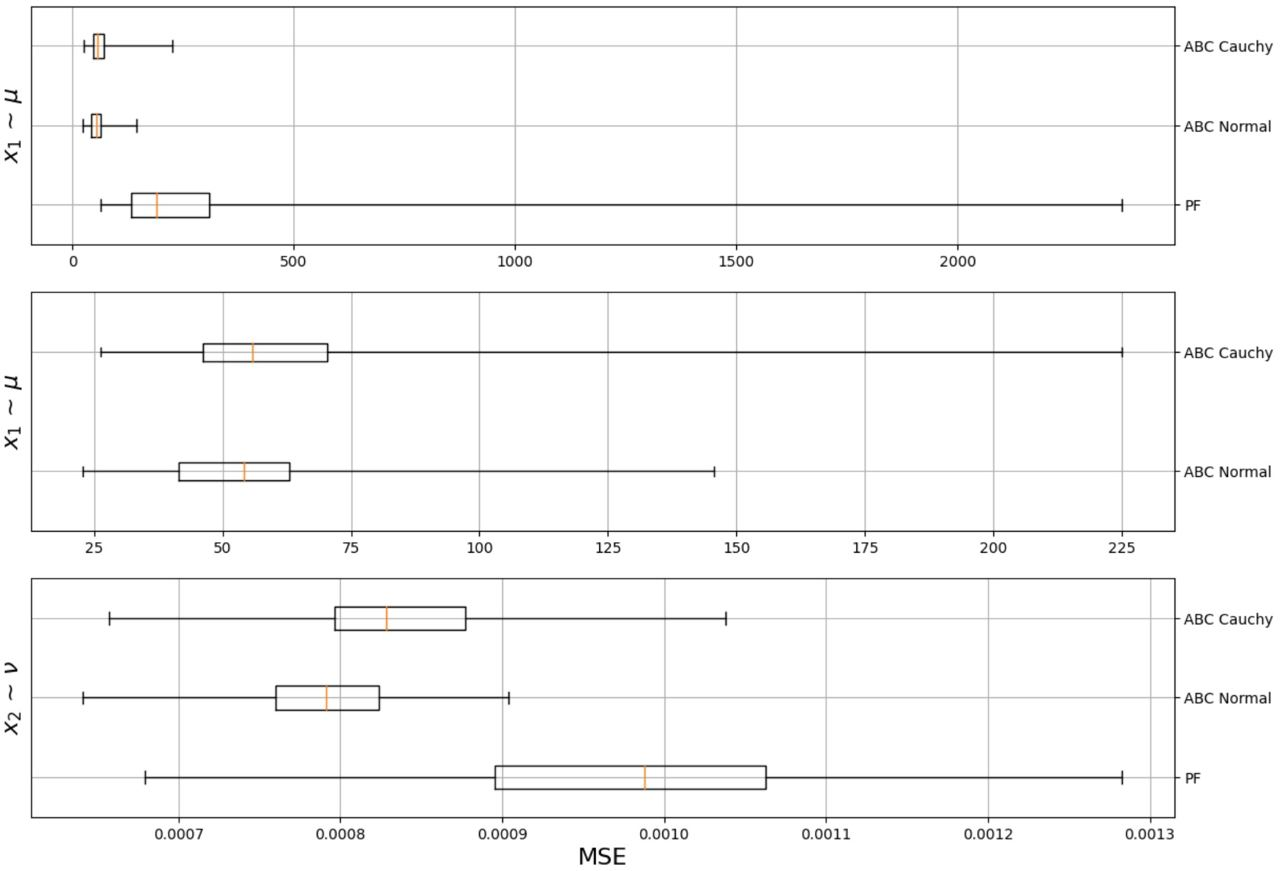
\includegraphics[width=0.9\columnwidth, height=\textheight,keepaspectratio]{figures/pgm/mse_boxplot_cauchy.jpg}}
\label{fig:pgm_mse_boxplot_cauchy}
\end{figure}

\begin{table}[h!]
\centering
\begin{tabular}{ |p{4cm}|p{4cm}|p{4cm}|}
 \hline 
  & \(\mu\) & \(\nu\)\\
 \hline \hline
 EKF & - & - \\
 PF & 271.668  & 9.830e-04 \\
 ABC Normal & 56.660 & 7.899e-04\\
 ABC Cauchy & 64.265 & 8.366e-04\\
 \hline
\end{tabular}
\caption{(PGM, Cauchy noise) The final MSE values for both state variables \(\mu\) and \(\nu\) averaged over 100 runs}
\label{table:pgm_mse_cauchy}
\end{table}

Figure \ref{fig:pgm_measurement_noise_cauchy} shows a noise realization from one of the 100 experiments. A noise time series for a single experiment run is shown in Figure \ref{fig:pgm_abc_scales_evolution_cauchy}, along with evolutions of the normal and Cauchy kernel scales. From the example of this data, it is well seen that both ABC filters reflect well the noise evolution, regardless of the choice of kernel.

\begin{figure}[!ht]
\centering
\caption{(PGM, Cauchy noise) One particular Cauchy noise realization \(\varepsilon_t\). Relative frequency histogram limited to [-120; 120] and scale-broken box plot. The box plot consists of three parts. The central part is a box that includes the median, upper and lower quartiles. The length of the whiskers is defined as 1.5 times the interquartile range. Outliers and extreme values are displayed on the left and right, respectively.}
\subfloat{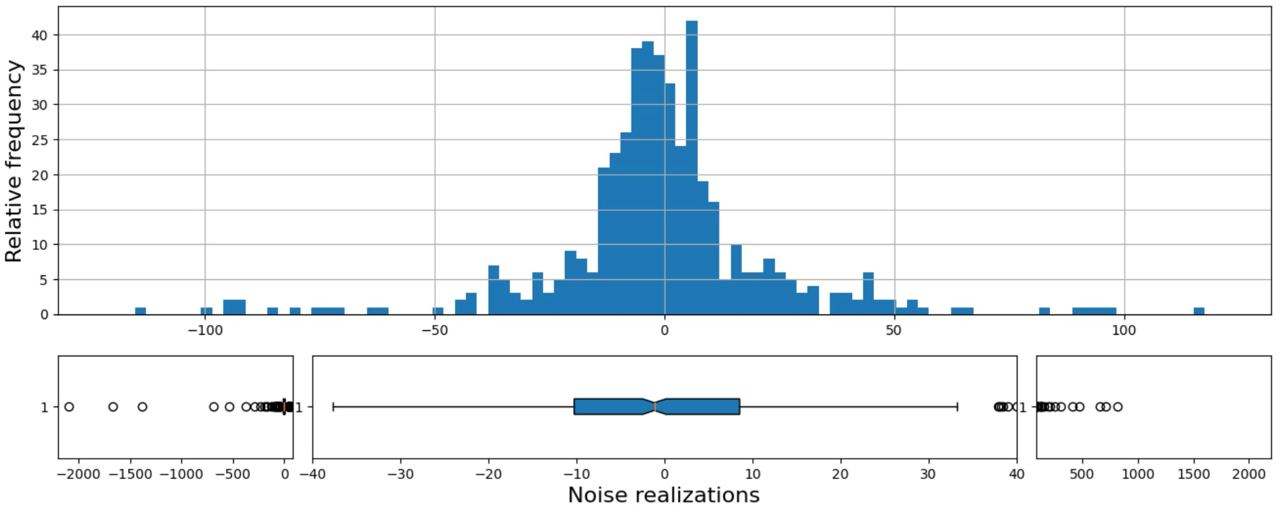
\includegraphics[width=0.9\columnwidth, height=\textheight,keepaspectratio]{figures/pgm/measurement_noise_cauchy.jpg}}
\label{fig:pgm_measurement_noise_cauchy}
\end{figure}

\begin{figure}[!ht]
\centering
\caption{(PGM, Cauchy noise) The top two graphs show the one particular evolution of the normal and Cauchy scales \(\varepsilon_t\), respectively. The lower one represents the Cauchy noise realizations.}
\subfloat{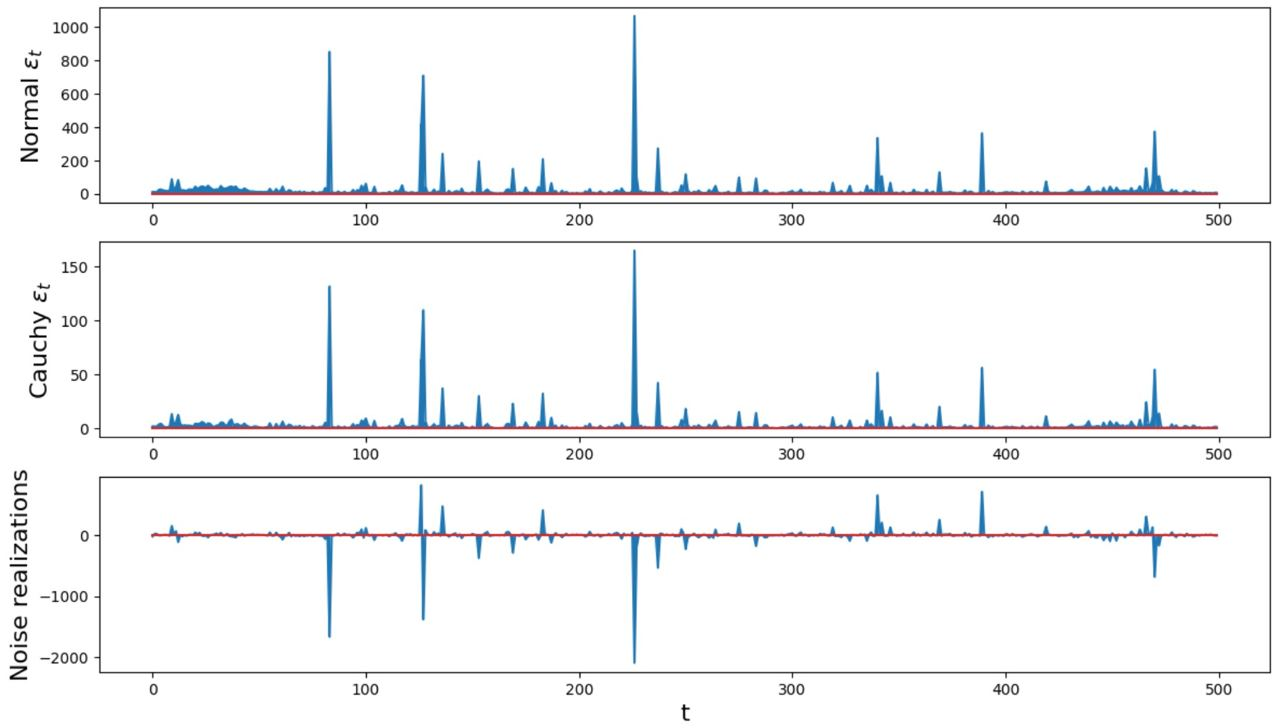
\includegraphics[width=0.9\columnwidth, height=\textheight,keepaspectratio]{figures/pgm/abc_scales_evolution_cauchy.jpg}}
\label{fig:pgm_abc_scales_evolution_cauchy}
\end{figure}

\section{Example 2: Constant velocity model}
In this section, the discussion will focus on the model already described earlier, namely the CVM. The model itself is characterized by the following equations (\ref{eq:cvm_equations}) and (\ref{eq:cvm_measurement_equation}). As mentioned earlier, the initialization parameters of the filters are not changed the same way as the constructed SSM. Also, the same measurement model is used (\ref{eq:cvm_measurement_model}), but all measurements in this example are corrupted by Cauchy distributed noise instead of Gaussian, keeping the same scaling parameter:

\begin{equation}
\begin{aligned}
\varepsilon_t \sim \mathcal{C}\text{auchy}\left(0, R_t\right) \quad \text{with} \quad R =
    3^{2}\cdot
    \begin{bmatrix}
        1 & 0 \\
        0 & 1
    \end{bmatrix}
\end{aligned}
\end{equation}

In order to obtain representative results, an experiment with 100 repetitions was conducted. 

\paragraph*{Charts and analysis}
Following the already usual approach, the analysis will focus on the MSE values, which can be found in Figure \ref{fig:cvm_mse_boxplot_cauchy} representing the statistic of the final MSE values of 100 repeated experiment runs, and in Table \ref{table:cvm_mse_cauchy}, which shows their averaged values.

Again it can be noted that, in general, the ABC filters showed the best results among the other filters, in the predominant number of repetitions of the experiment had the minimum final MSE, which is also well reflected in the Table of averaged values. The ABC filter in the normal kernel was closer to the true values when tracing, which can be seen in all box plots, and as a consequence, it has lower values of the averaged MSE for all state variables compared to the ABC filter with the Cauchy kernel. But on the whole, the ABC filter with the Cauchy kernel also showed decent results in the prevailing number of runs of the experiment.

As for the PF filter, it can be safely said that it had enough trouble tracking all state variables, which is reflected in its MSE values. If in the context of this experiment, ABC filters with both kernels showed themselves as relatively stable under heavy-tailed noise, the same cannot be said about the PF filter.

Regarding the KF filter and box plots of its final MSE values, it can be stated that in the majority of cases, the filter was quite accurate in tracking, but judging by the maximum final MSE values, which are very far from the medians on all box plots, one can judge that in some rare runs the filter absolutely failed. That also confirms the statement about its non-optimality under the given conditions. The consequence of the maximum MSE values is also displayed on the averaged MSE values in the Table \ref{table:cvm_mse_cauchy}.

\begin{figure}[!ht]
\centering
\caption{(CVM, Cauchy noise)  Box plots showing final MSE values for all state variables $x_1$, $x_2$, $v_1$ and $v_2$ of 100 repeated experiments. The boxes show medians, upper and lower quartiles. The length of the whiskers is defined as 1.5 times the interquartile range. The outliers are not displayed.}
\subfloat{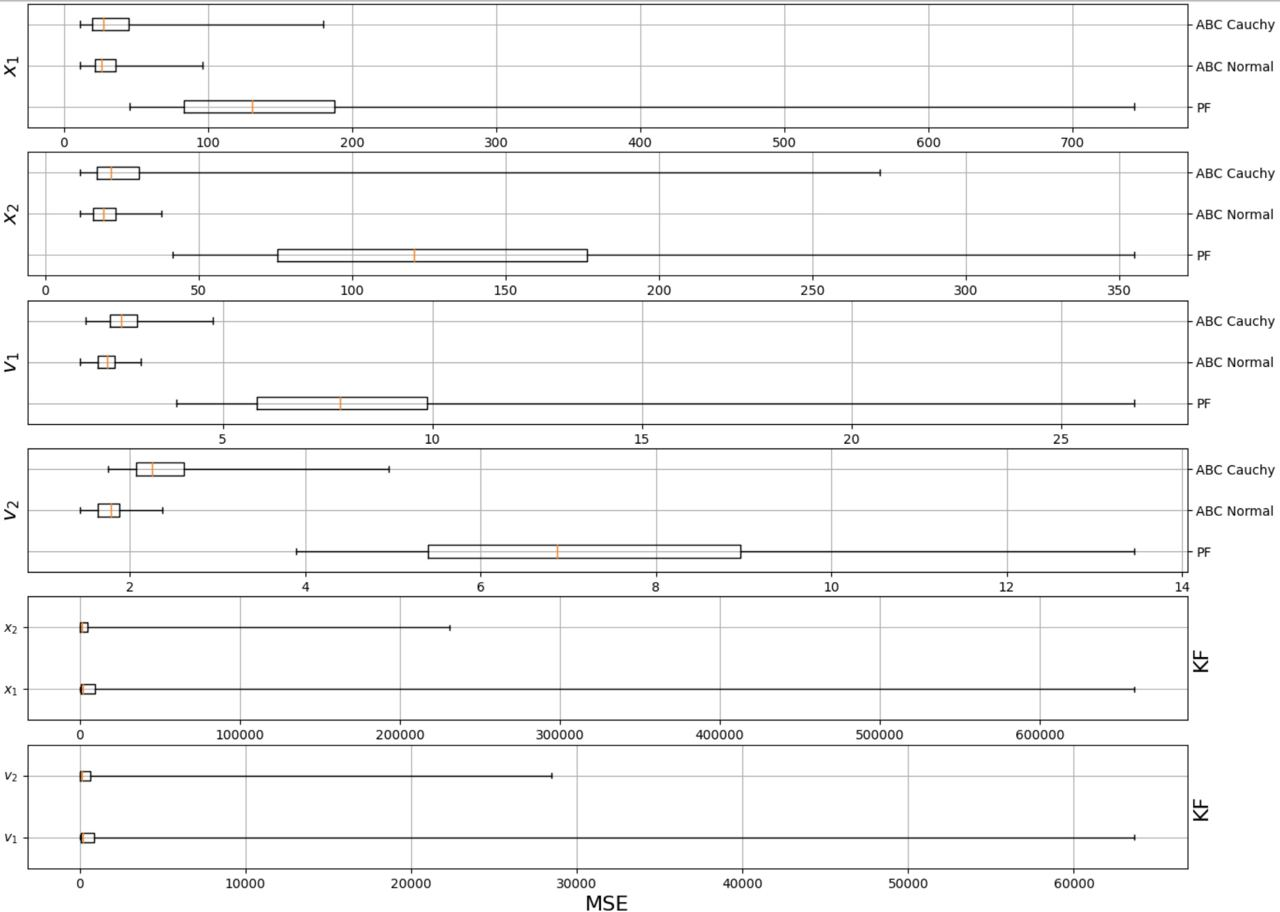
\includegraphics[width=0.9\columnwidth, height=\textheight,keepaspectratio]{figures/cvm/mse_boxplot_cauchy.jpg}}
\label{fig:cvm_mse_boxplot_cauchy}
\end{figure}

\begin{table}[h!]
\centering
\begin{tabular}{ |p{2cm}|p{2cm}|p{2cm}|p{2cm}|p{2cm}|}
 \hline 
  & $x_1$ & $x_2$ & $v_1$ & $v_2$ \\
 \hline \hline
 KF & 303.669e+03 & 268.659e+07 & 294.374e+02 & 259.620e+06  \\
 PF & 162.614 & 129.882 & 8.701 & 7.302 \\
 ABC Normal & 29.952 & 19.894 & 2.244 & 1.781 \\
 ABC Cauchy & 38.065 & 29.674 & 2.721 & 2.390 \\
 \hline
\end{tabular}
\caption{(CVM, Cauchy noise) The final MSE values for all state variables $x_1$, $x_2$, $v_1$ and $v_2$ averaged over 100 runs}
\label{table:cvm_mse_cauchy}
\end{table}


Again, to evaluate the effectiveness of ABC filters, it is worth looking at Figure \ref{fig:cvm_measurement_noise_cauchy}, which shows a noise realization from one of the 100 experiments, and also, at  Figure \ref{fig:cvm_abc_scales_evolution_cauchy} which shows a noise time series for a single experiment run, along with evolutions of the normal and Cauchy kernel scales. It is clear that both ABC filters reflect well the noise evolution, even the significant values.

\begin{figure}[!ht]
\centering
\caption{(CVM, Cauchy noise) One particular Cauchy noise realizations \(\varepsilon_{y_1,t}\) and \(\varepsilon_{y_2,t}\). Relative frequency histograms limited to [-60; 60] and scale-broken box plots. Each box plot consists of three parts. The central part is a box that includes the median, upper and lower quartiles. The length of the whiskers is defined as 1.5 times the interquartile range. Outliers and extreme values are displayed on the left and right, respectively.}
\subfloat{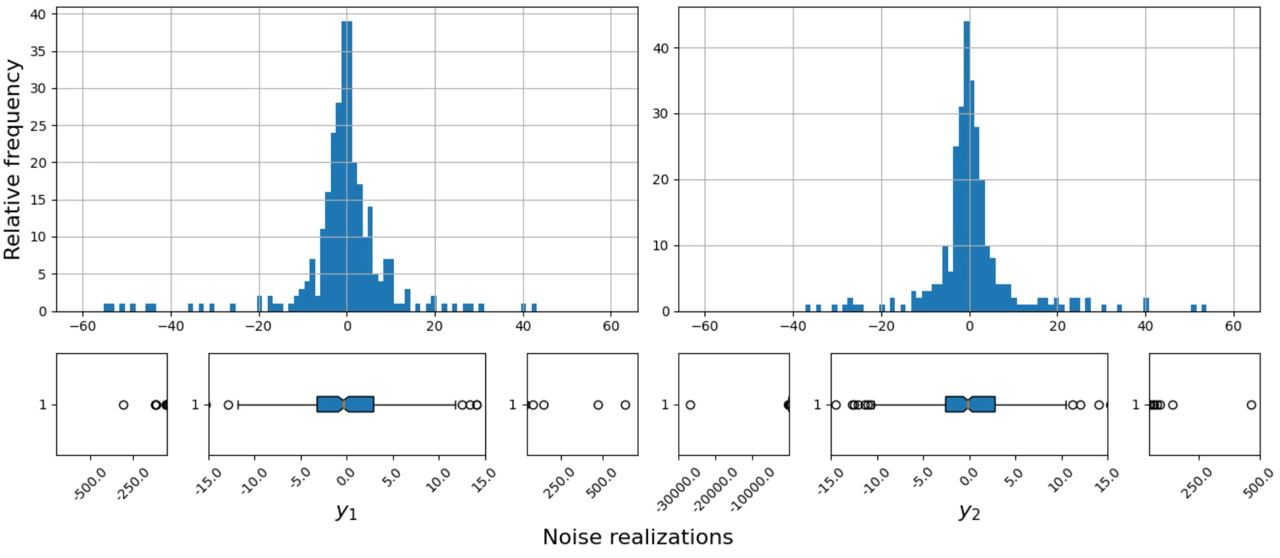
\includegraphics[width=0.9\columnwidth, height=\textheight,keepaspectratio]{figures/cvm/measurement_noise_cauchy.jpg}}
\label{fig:cvm_measurement_noise_cauchy}
\end{figure}

\begin{figure}[!ht]
\centering
\caption{(CVM, Cauchy noise) The top four graphs show the one particular evolution of the normal and Cauchy scales \(\varepsilon_{y_1,t}, \varepsilon_{y_2,t}\), respectively. The bottom two represent the Cauchy noise realizations.}
\subfloat{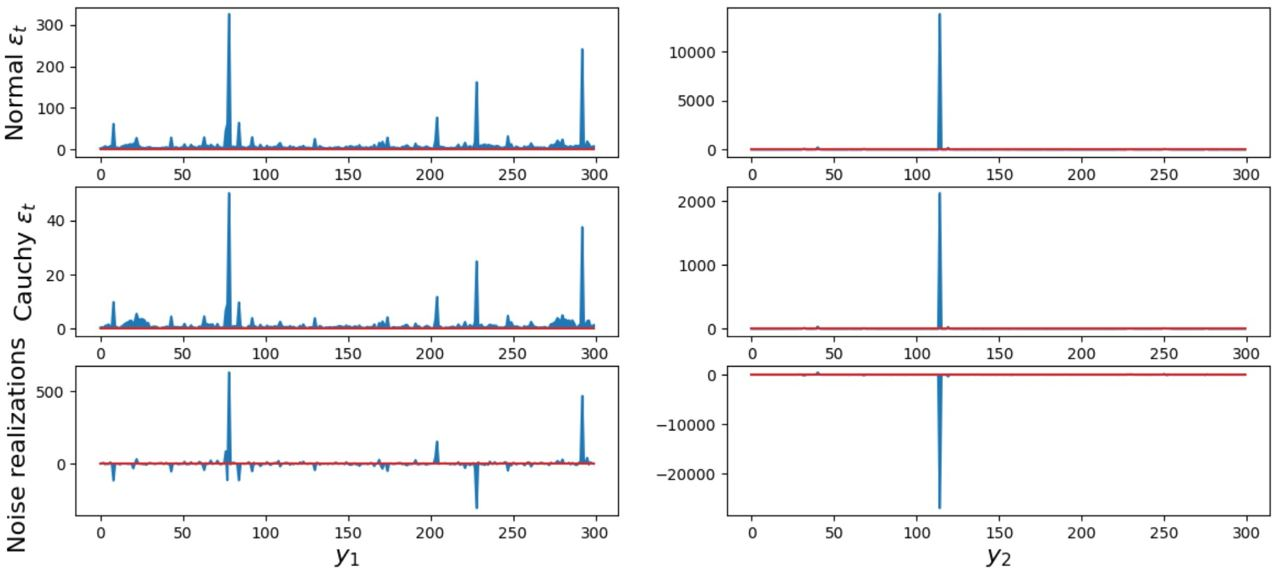
\includegraphics[width=0.9\columnwidth, height=\textheight,keepaspectratio]{figures/cvm/abc_scales_evolution_cauchy.jpg}}
\label{fig:cvm_abc_scales_evolution_cauchy}
\end{figure}

\section{Example 3: Polar radar model}
Returning to the PRM, which is described by the following equations (\ref{eq:cvm_equations}) and (\ref{eq:prm_equations}), leaving everything unchanged for the honesty of the experiment, except that all measurements will be corrupted by Cauchy distributed noise. In addition, the initialization parameters of the filters are not changed. The same noise scale parameter remains. The measurement noise is as follows:

\begin{equation}
    \varepsilon_t \sim \mathcal{C}\text{auchy}\left(0, R_t\right) \quad \text{with} \quad R =
    3^{2}\cdot
    \begin{bmatrix}
        0.01 & 0.0 & 0.0 \\
        0.0 & 0.0001 & 0.0 \\
        0.0 & 0.0 & 0.01
    \end{bmatrix}.
\end{equation}

In order to obtain representative results, an experiment with 100 repetitions was conducted.

\paragraph*{Charts and analysis}
As can be expected that the analysis will focus on the MSE values, which can be found in Figure \ref{fig:prm_mse_boxplot_cauchy}, which shows the statistics of the final MSE values of 100 repeated experiment runs, and in Table \ref{table:prm_mse_cauchy}, which contains their averaged values.

One can observe approximately the same situation as in the previous expert. But this time, both ABC filters really showed outstanding results. Minimal averaged MSE values in Table \ref{table:prm_mse_cauchy} show high robustness to different heavy noise realizations. It is worth noting that in the context of this experiment, the ABC filter with the Cauchy kernel performed slightly but better than the same filter with the normal kernel and generally has lower MSE values. It is also worth noting that the choice of the kernel has no significant impact on the effectiveness of the ABC filter.

As for the PF filter, the tendency for it to be inferior to ABC filters in this chapter continues, which is logical since it assumes a misspecified measurement model with normal noise. In general, it always has a much larger final MSE value, and at times, judging by the maximum values from the box plots, they are even critically significant. This is also reflected in the averaged values in the table \ref{table:prm_mse_cauchy}, especially for the state variables \(x_1\) and \(x_2\).

The last thing that has not been analyzed is the tracking efficiency of the EKF filter. It can be definitely said that the EKF filter suffered the same fate as the KF filter in the previous section within the CVM experiments.
That is, the prevailing number of runs EKF was quite close to the true values in its estimation process, but judging by the maximum values from the box plots, in rare cases, the final MSE values were critically high, which also affected the averaged MSE values in the Table \ref{table:prm_mse_cauchy}. That also confirms and indicates that the EKF filter is quite unstable under some heavy-tailed noise realizations.

\begin{figure}[!ht]
\centering
\caption{(PRM, Cauchy noise) Box plots showing final MSE values for all state variables $x_1$, $x_2$, $v_1$ and $v_2$ of 100 repeated experiments. The boxes show medians, upper and lower quartiles. The length of the whiskers is defined as 1.5 times the interquartile range. The outliers are not displayed.}
\subfloat{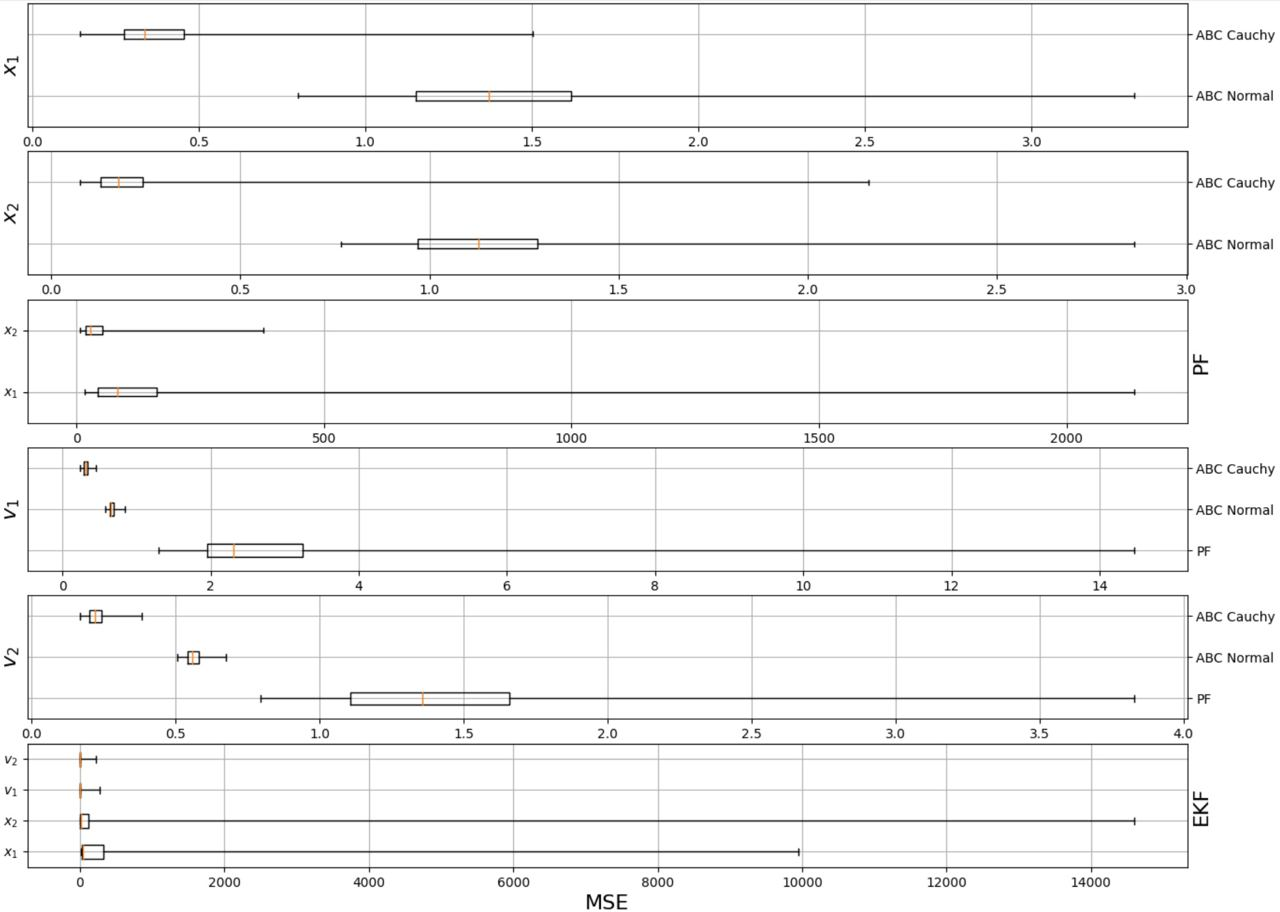
\includegraphics[width=0.9\columnwidth, height=\textheight,keepaspectratio]{figures/prm/mse_boxplot_cauchy.jpg}}
\label{fig:prm_mse_boxplot_cauchy}
\end{figure}

\begin{table}[h!]
\centering
\begin{tabular}{ |p{2cm}|p{2cm}|p{2cm}|p{2cm}|p{2cm}|}
 \hline 
  & $x_1$ & $x_2$ & $v_1$ & $v_2$ \\
 \hline \hline
 EKF & 620.381 & 466.478 & 15.570 & 10.575  \\
 PF & 184.171  & 48.923 & 3.017 & 1.484 \\
 ABC Normal & 1.450 & 1.182 & 0.664 & 0.562 \\
 ABC Cauchy & 0.401 & 0.222 & 0.316 & 0.227 \\
 \hline
\end{tabular}
\caption{(PRM, Cauchy noise) The final MSE values for all state variables $x_1$, $x_2$, $v_1$ and $v_2$ averaged over 100 runs}
\label{table:prm_mse_cauchy}
\end{table}

The Figure \ref{fig:prm_measurement_noise_cauchy} shows a noise realization from one of the 100 experiments. To evaluate how well the ABC filter with different kernels reflects the noise evolution is enough to look at Figure \ref{fig:cvm_abc_scales_evolution_cauchy}, which shows a noise time series for a single experiment run, along with evolutions of the normal and Cauchy kernel scales. It is absolutely clear that the ABC filter with both kernels captures noise evolution well.

\begin{figure}[!ht]
\centering
\caption{(PRM, Cauchy noise) One particular normal noise realizations \(\varepsilon_{y_1,t}\), \(\varepsilon_{y_2,t}\) and \(\varepsilon_{y_3,t}\). Relative frequency histograms and scale-broken box plots. The histograms on the sides are limited to [-0.4,0.4], and the middle one is limited to [-0.004,0.004]. Each box plot consists of three parts. The central part is a box that includes the median, upper and lower quartiles. The length of the whiskers is defined as 1.5 times the interquartile range. Outliers and extreme values are displayed on the left and right, respectively.}
\subfloat{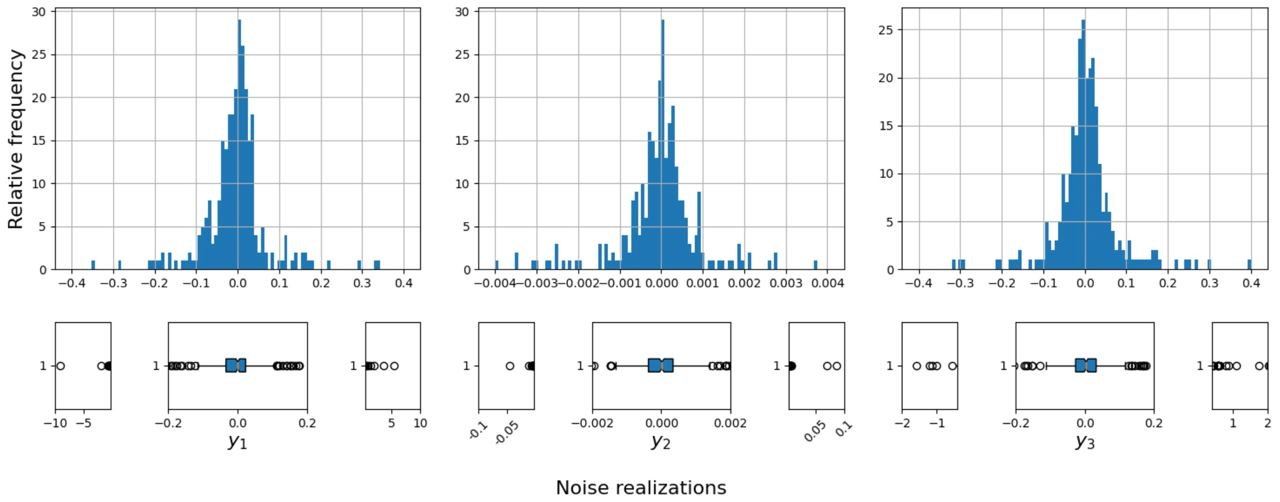
\includegraphics[width=0.9\columnwidth, height=\textheight,keepaspectratio]{figures/prm/measurement_noise_cauchy.jpg}}
\label{fig:prm_measurement_noise_cauchy}
\end{figure}

\begin{figure}[!ht]
\centering
\caption{(PRM, Cauchy noise) The top four graphs show the one particular evolution of the normal and Cauchy scales \(\varepsilon_{y_1,t}, \varepsilon_{y_2,t}\), and \(\varepsilon_{y_3,t}\), respectively. The bottom three represent the Cauchy noise realizations.}
\subfloat{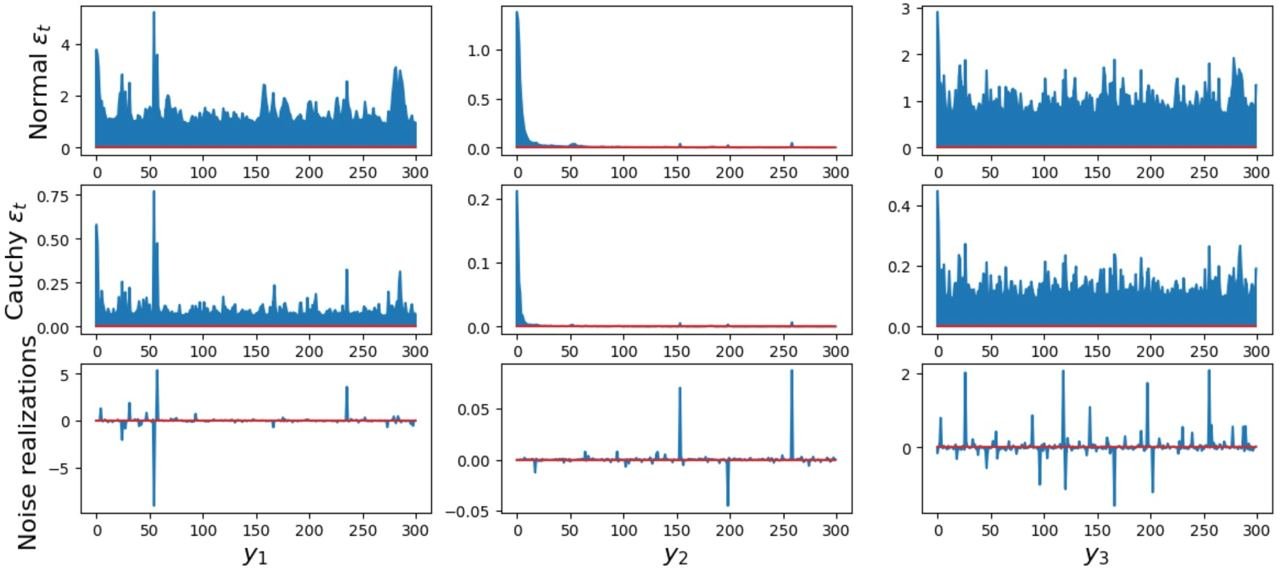
\includegraphics[width=0.9\columnwidth, height=\textheight,keepaspectratio]{figures/prm/abc_scales_evolution_cauchy.jpg}}
\label{fig:prm_abc_scales_evolution_cauchy}
\end{figure}

\section{Experiments conclusion}
It can be summarized that, within the framework of this chapter, the results of experiments showed the absolute superiority of ABC filters over the others in the conditions that the measurement model is misspecified, namely in conditions of ignorance of the noise of measurement distribution. It would be relevant to emphasize the stability of ABC filters again under different realizations of heavy-tailed noise, regardless of the choice of kernel.

%---------------------------------------------------------------
%---------------------------------------------------------------
% Conclusion
%---------------------------------------------------------------
\chapter{Conclusion}
\label{chap:conclusion}
%---------------------------------------------------------------
This thesis considers the sequential inference of state-space models using the Bayesian framework. The principle of the state-space representation itself approaches to modeling, and examples of use were examined in detail. Also considered was the very concept of Bayesian statistical inference, as finding the posterior distribution of states based on a sequence of observations as well as initial knowledge of the states called prior density. This included consideration of the most popular and widespread implementation of Bayesian filtering, filters from the Kalman family. Starting with the theory of linear systems, possible nonlinearities in systems were also touched upon, including completely nonlinear systems, including the possibility of applying the Kalman filter in the context of nonlinearity, or rather its extended version, and the principle of this application itself. It also questioned the possible difficulties with the inference process associated with an under-specified model and, accordingly, how this might affect the efficiency of the KFs.

Further, separate attention was paid to an alternative, but no less popular technique of state filtering, the class of SMC filters, namely the PF, which, due to the very idea of approximately representing required distribution by random samples, was supposed to show itself more stable in the context of misspecified models. But still, it also requires the measurement model to be a well-defined probability density, which is not possible in all applications. Given the dependence of the PF filter on knowledge of the measurement model, a more flexible approach, called ABC, which just might be used to bypass this requirement, was also studied and discussed.

Thus was derived an ABC filter with an adaptive kernel, which stands on the rails of the SMC filter, but uses an already approximated likelihood function in the update step. The concept of kernel usage and several possible types of commonly used kernels were also discussed.

All of the above was a good theoretical basis before proceeding directly to the experimental part. The experiments were performed with multiple repetitions to obtain representative results, and three different models and all of the filters and their variations listed above were used in the experiment. As for the comparison of the filters themselves, comparing the PF filter and the standard filters from the Kalman family, it can be safely said that as the number of particles used increases, so does the computational complexity, but thus the final results are more accurate. As for the obtained ABC filter with the adaptive kernel, we can conclude that it does not introduce any additional computational complexity compared to the PF. It is also important to note the fact that, while the model is highly nonlinear, the extended version of KF has a rather high computational cost for calculating the Jacobian matrix.

As for the performance and robustness of the filters themselves after the experiments, it can be safely stated the following theses. As for experiments on well-specified models, provided guaranteed linearity, and when both state and measurement models are linear with zero mean Gaussian noise, in this case, KF is still the best linear estimator, which showed the best results and, unlike other filters, is the cheapest in use. In the case of a nonlinear but well-defined model, it is better to use PF, as opposed to EKF, which, when one of the steps, either prediction or update, is highly nonlinear, will have relatively poor performance. It is also worth noting that the ABC filter with different kernels showed itself very competitively, but all were noticeably inferior to both the KF filter and the PF. In general, it can be argued that the results of the experiments revealed that the ABC filter is not overly sensitive to kernel choice, regardless of model specification.

Regarding experiments with misspecified models, and more specifically, in the context of the misspecified measurement model, the ABC filter, regardless of the kernel choice, proved unsurpassed. It is also pertinent to emphasize the particular robustness of ABC filters in different realizations of heavy-tailed noise.

As for possible ideas and extensions for future works, one of the main directions will be formulating the adaptive kernel tuning to multiple dimensions. For as already noted, within this thesis, most of the models had multidimensional measurement values, but the procedure of tuning itself was done in the context of one-dimensional kernels, handling multidimensional data in a coordinate-wise manner. The consequence of this is that the individual measurement vector elements are assumed to be independent. Also, a good solution for future work would be to take both more complex and as simple models as possible to make a comparison still in this context. And, of course, expanding the list of filters used in the experiments would be nice.
%---------------------------------------------------------------

\appendix\appendixinit % do not remove these two commands

\chapter{Acronyms}

% ¥printglossaries
\begin{description}
	\item[SSM] State-space model
    \item[HMM] Hidden Markov model
    \item[LTI] Linear time-invarian
    \item[SISO] Single Input Single Output
    \item[CT] Continuous-time
    \item[MIMO] Multi Input Mult Output
    \item[DT] Discrete-time
    \item[DLM] Dynamic linear model
    \item[MLE] Maximum likelihood estimation
    \item[RLS] Recursive least squares
    \item[MSE] Mean square error
    \item[SMC] Sequential Monte Carlo
    \item[CLT] Central limit theorem
    \item[IF] Importance function
    \item[ABC] Approximate Bayesian computation
    \item[HPR] Highest Probability Region
    \item[CDF] Cumulative distribution function
    \item[KF] Kalman filter
    \item[PF] Particle filter
\end{description}
 % include `appendix.tex' from `text/' subdirectory

\backmatter % do not remove this command

\printbibliography % print out the BibLaTeX-generated bibliography list

\chapter{Contents of the attached media}


	\dirtree{%
		.1 readme.txt\DTcomment{a brief description of the content of the medium}.
		.1 src.
		.2 impl\DTcomment{implementation source codes}.
		.2 thesis\DTcomment{source form of the thesis in format \LaTeX{}}.
		.1 text\DTcomment{the text of the thesis}.
		.2 thesis.pdf\DTcomment{text of the thesis in PDF format}.
	}
 % include `medium.tex' from `text/' subdirectory

\end{document}
